\chapter{Figuren van de observaties}\label{sec:figobservaties}
Dit hoofdstuk bevat de testdata op een grafische manier voorgesteld. Dit is enkel een selectie van de figuren, al de data en figuren kunnen gevonden worden op \url{https://github.com/thuys/YCSB-Testdata}.  
\begin{figure}[h!] 
\centering
	\subfigure[MongoDB]{\label{fig:calibratie-gebruikers-mongodb} \includegraphics[width=0.4\textwidth]{img/Observaties/threads-MongoDB}}
	\subfigure[Pgpool-II]{\label{fig:calibratie-gebruikers-pgpool-ii} 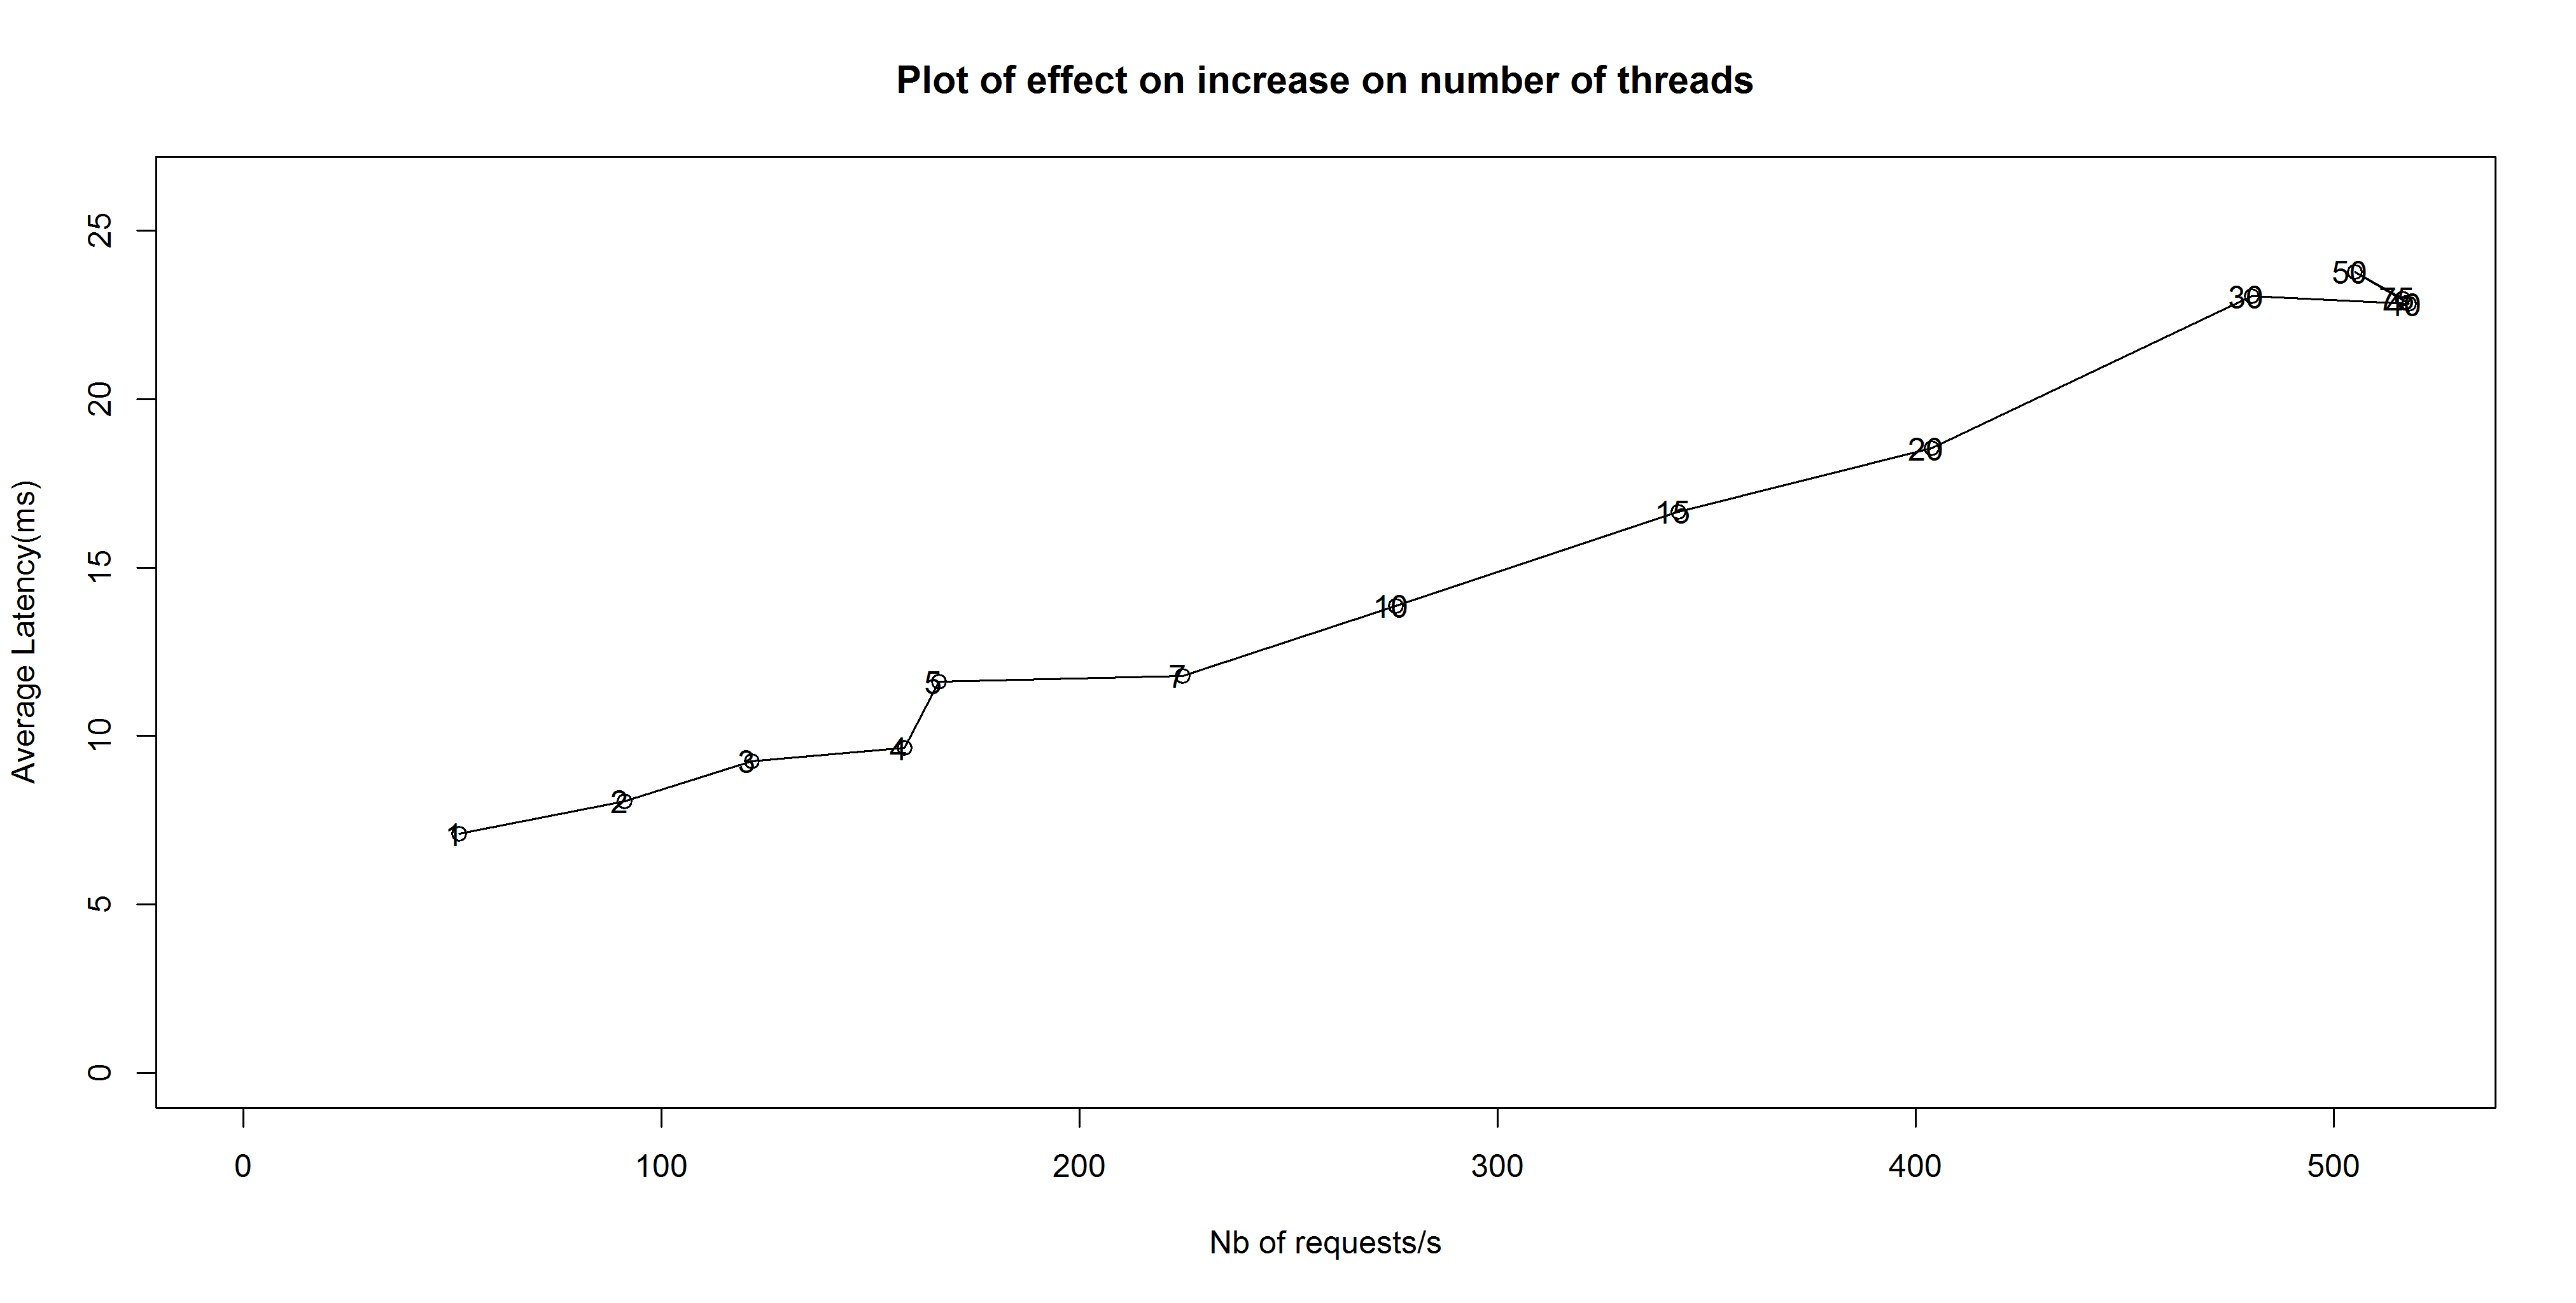
\includegraphics[width=0.4\textwidth]{img/Observaties/threads-postgresql}}
	\subfigure[HBase]{\label{fig:calibratie-gebruikers-hbase} \includegraphics[width=0.4\textwidth]{img/Observaties/threads-HBase}}
	\caption{Calibratie: Overzicht van het aantal queries tot de gemiddelde vertraging voor verschillend aantal gebruikers. Elk datapunt stelt een verschillend aantal gebruikers voor met het aantal rechtsboven het punt. }
	\label{fig:calibratie-gebruikers-resultaat}
\end{figure}

\begin{figure}[htb!] 
	\centering
	\subfigure{\label{fig:calibratie-queriesperseconde-hbase-1} 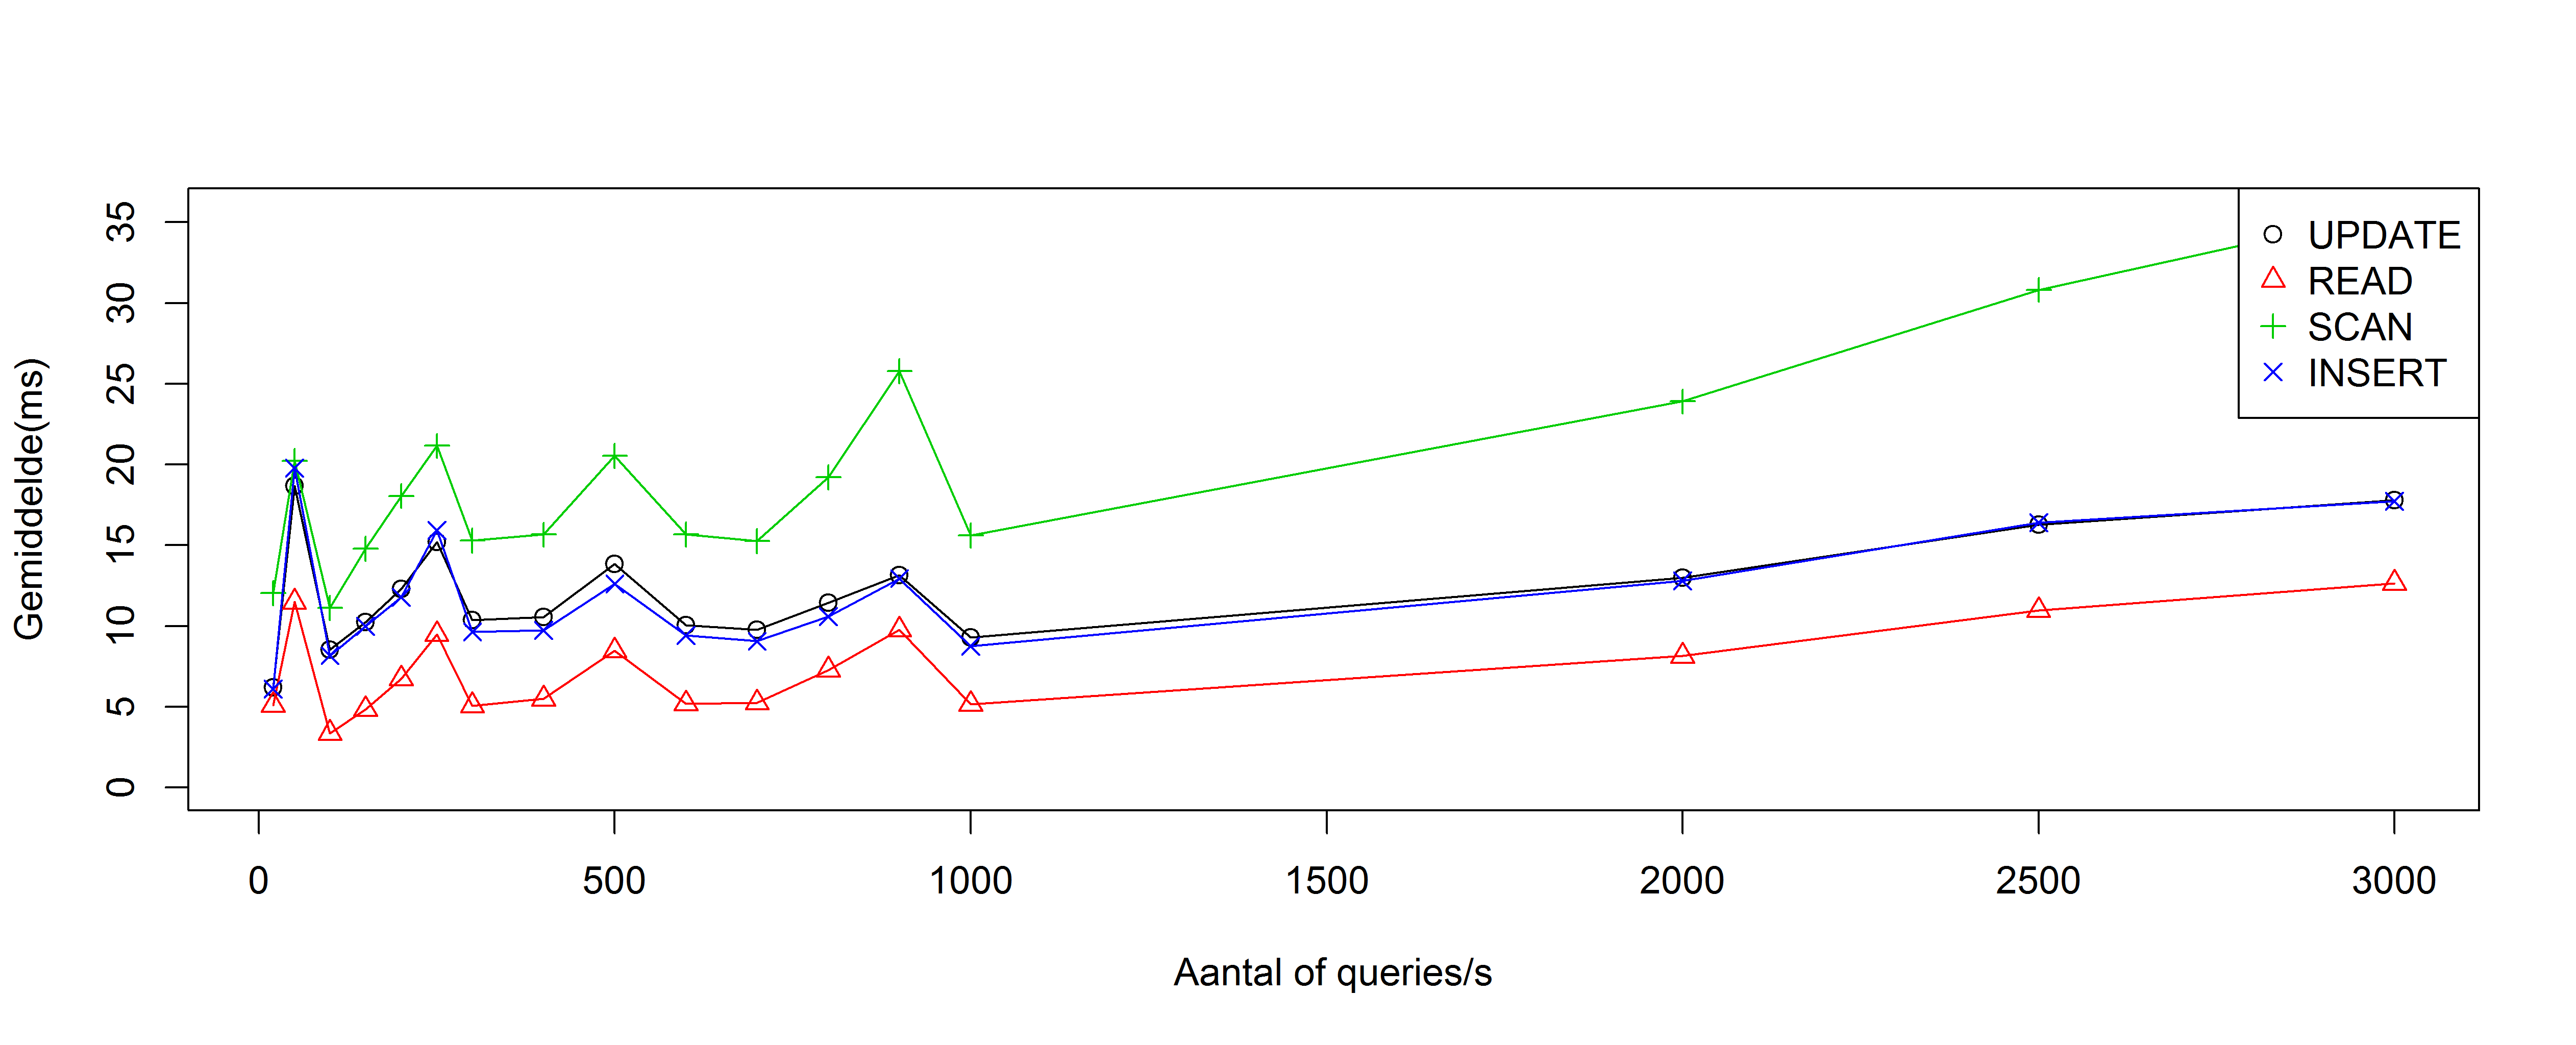
\includegraphics[width=0.95\textwidth]{img/Observaties/loadbalance-db-HBase}}
	\subfigure{\label{fig:calibratie-queriesperseconde-hbase-2} 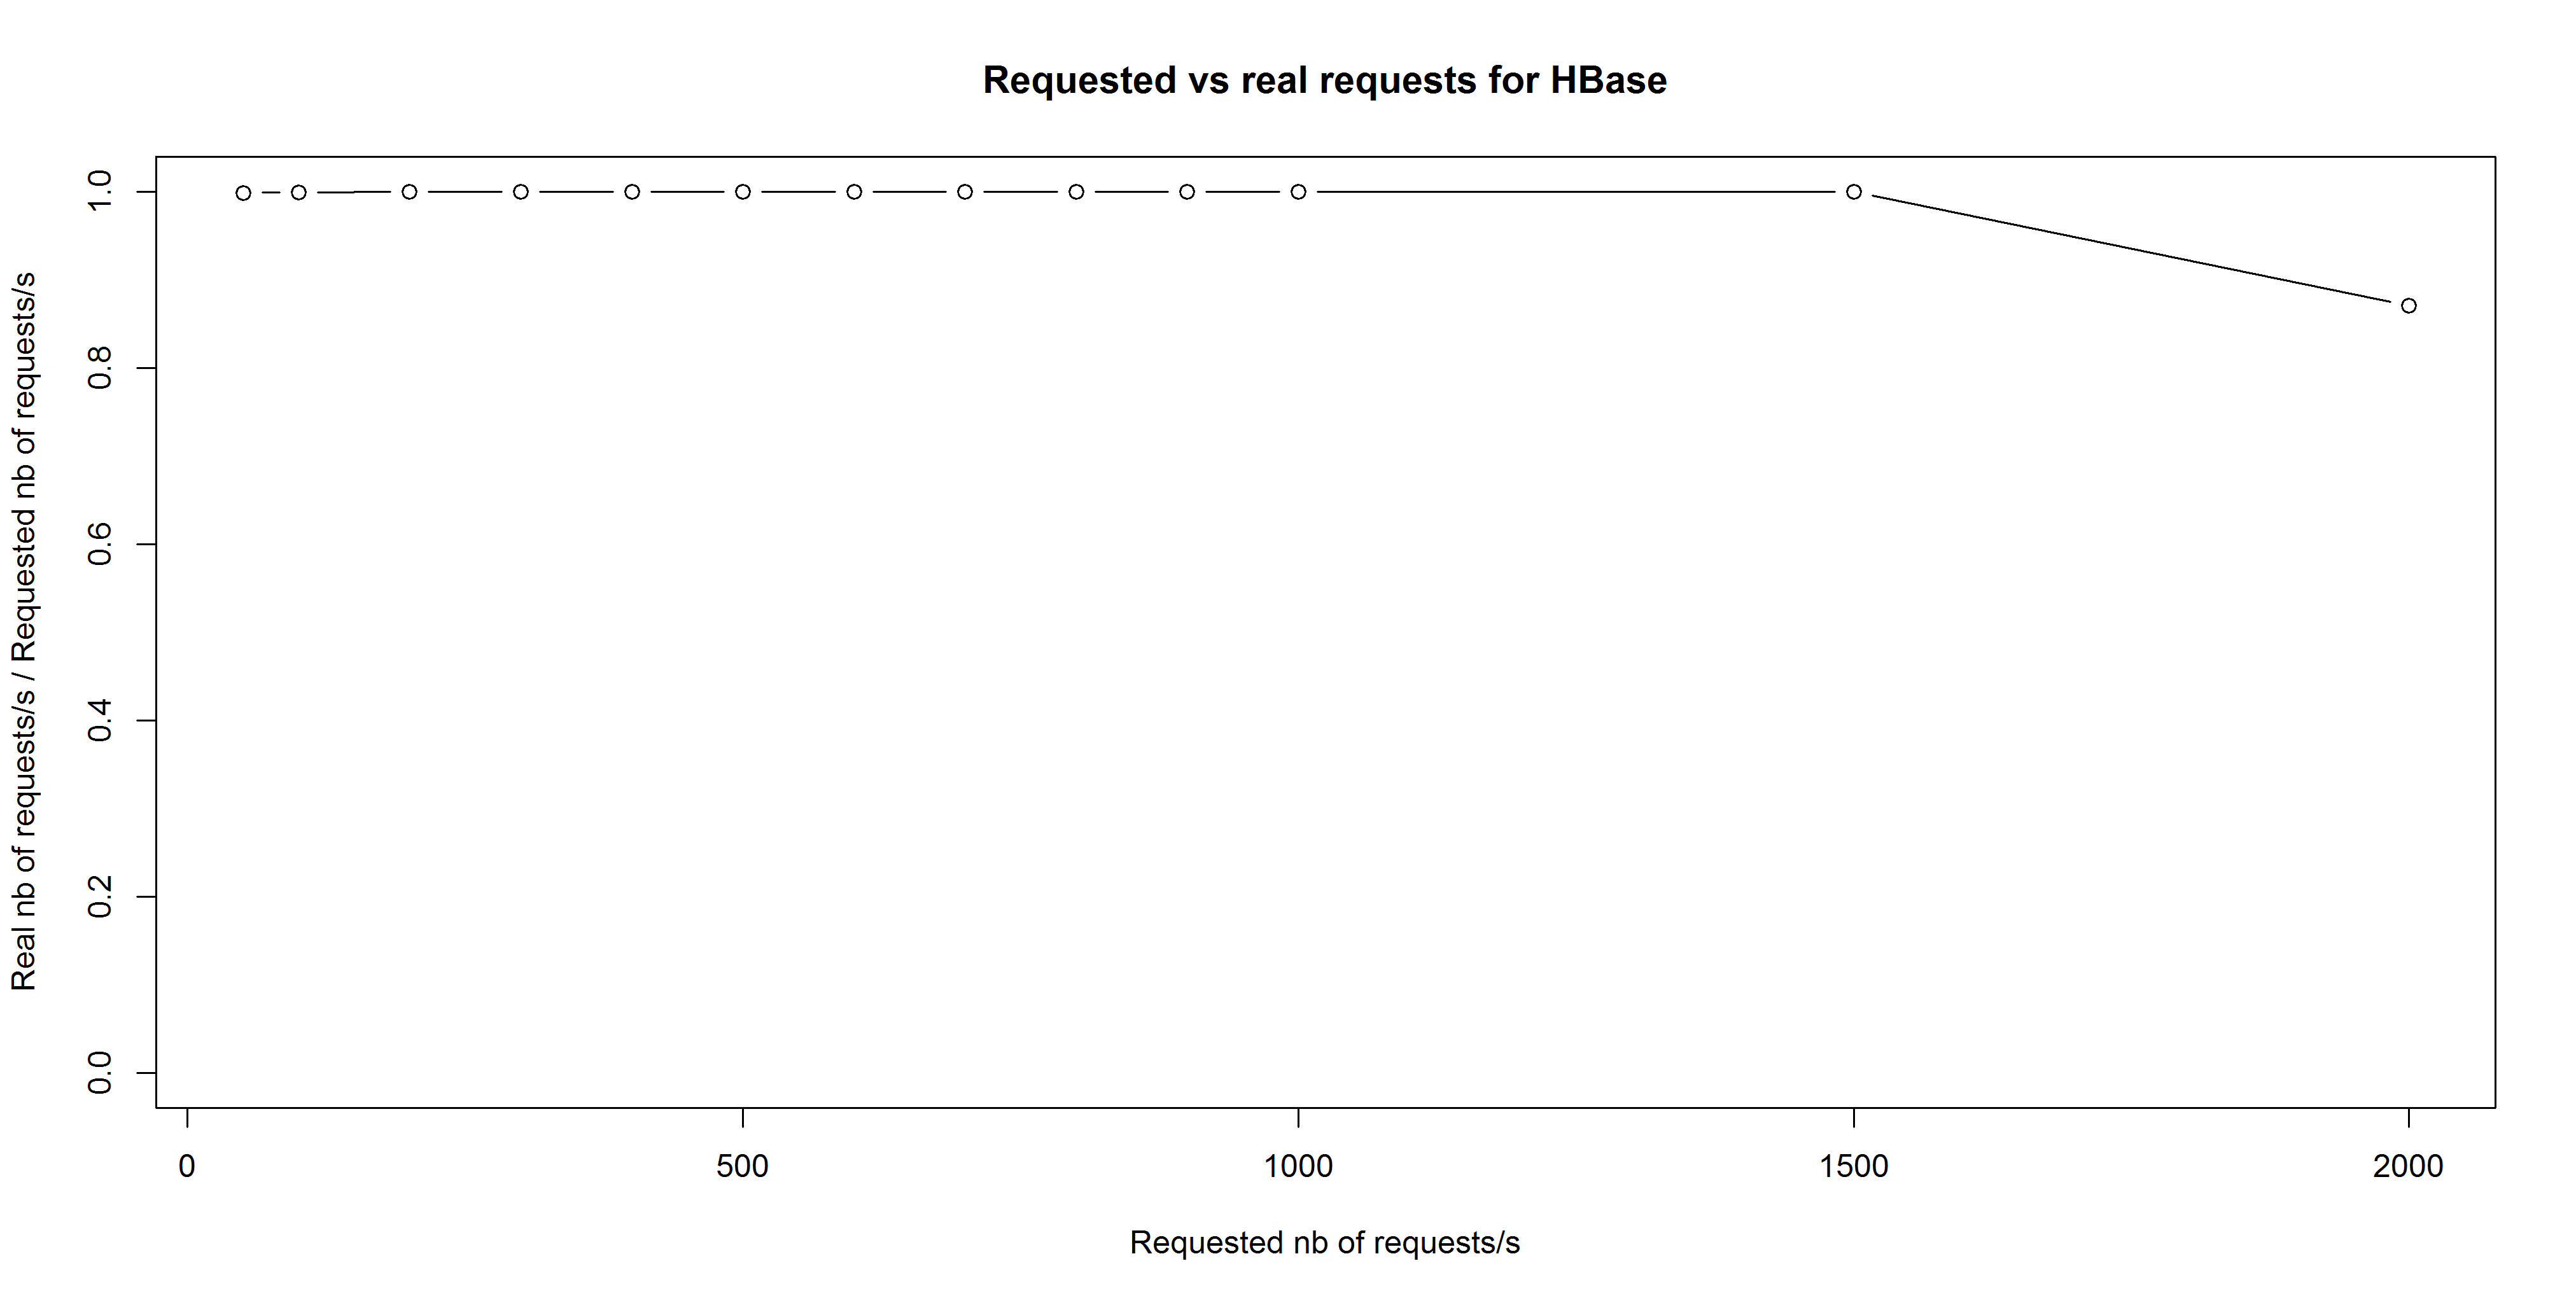
\includegraphics[width=0.95\textwidth]{img/Observaties/loadbalance-realthroughput-db-HBase}}
	\caption{Calibratie: Overzicht van de vertraging t.o.v. het theoretisch aantal aanvragen met een vergelijking hoeveel werkelijke aanvragen er waren voor HBase. }
	\label{fig:calibratie-queriesperseconde-hbase}
\end{figure}

\begin{figure}[htb!] 
	\centering
	\subfigure{\label{fig:calibratie-queriesperseconde-mongodb-1} 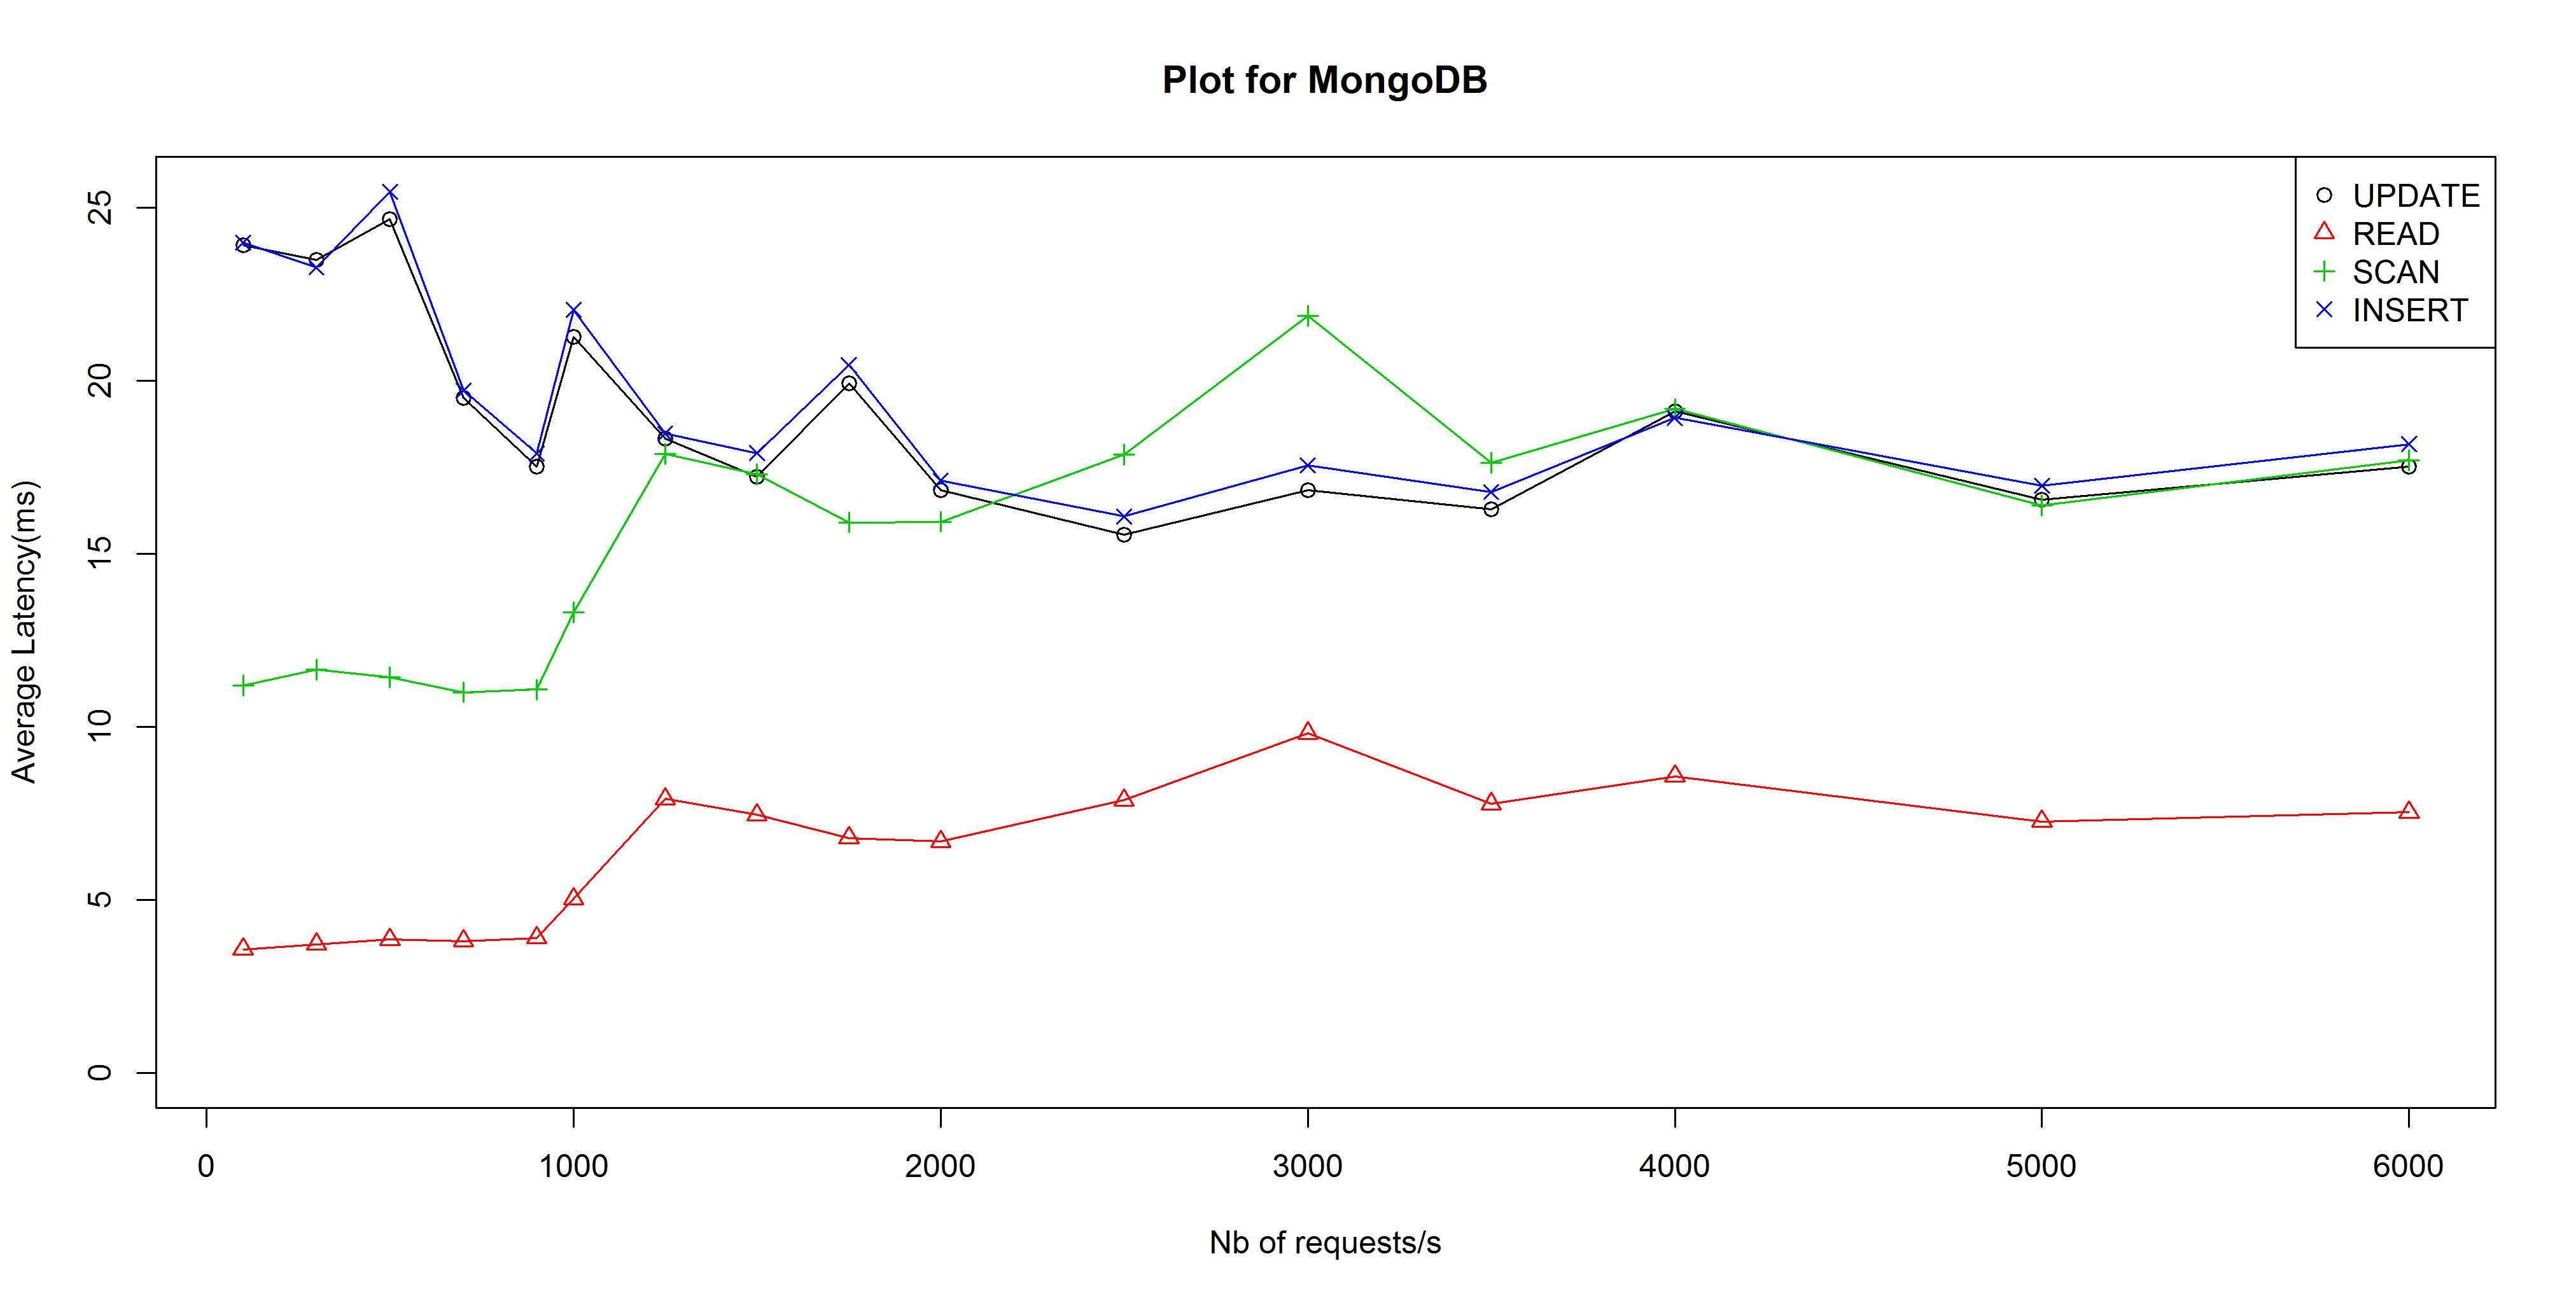
\includegraphics[width=0.95\textwidth]{img/Observaties/loadbalance-db-MongoDB}}
	\subfigure{\label{fig:calibratie-queriesperseconde-mongodb-2} 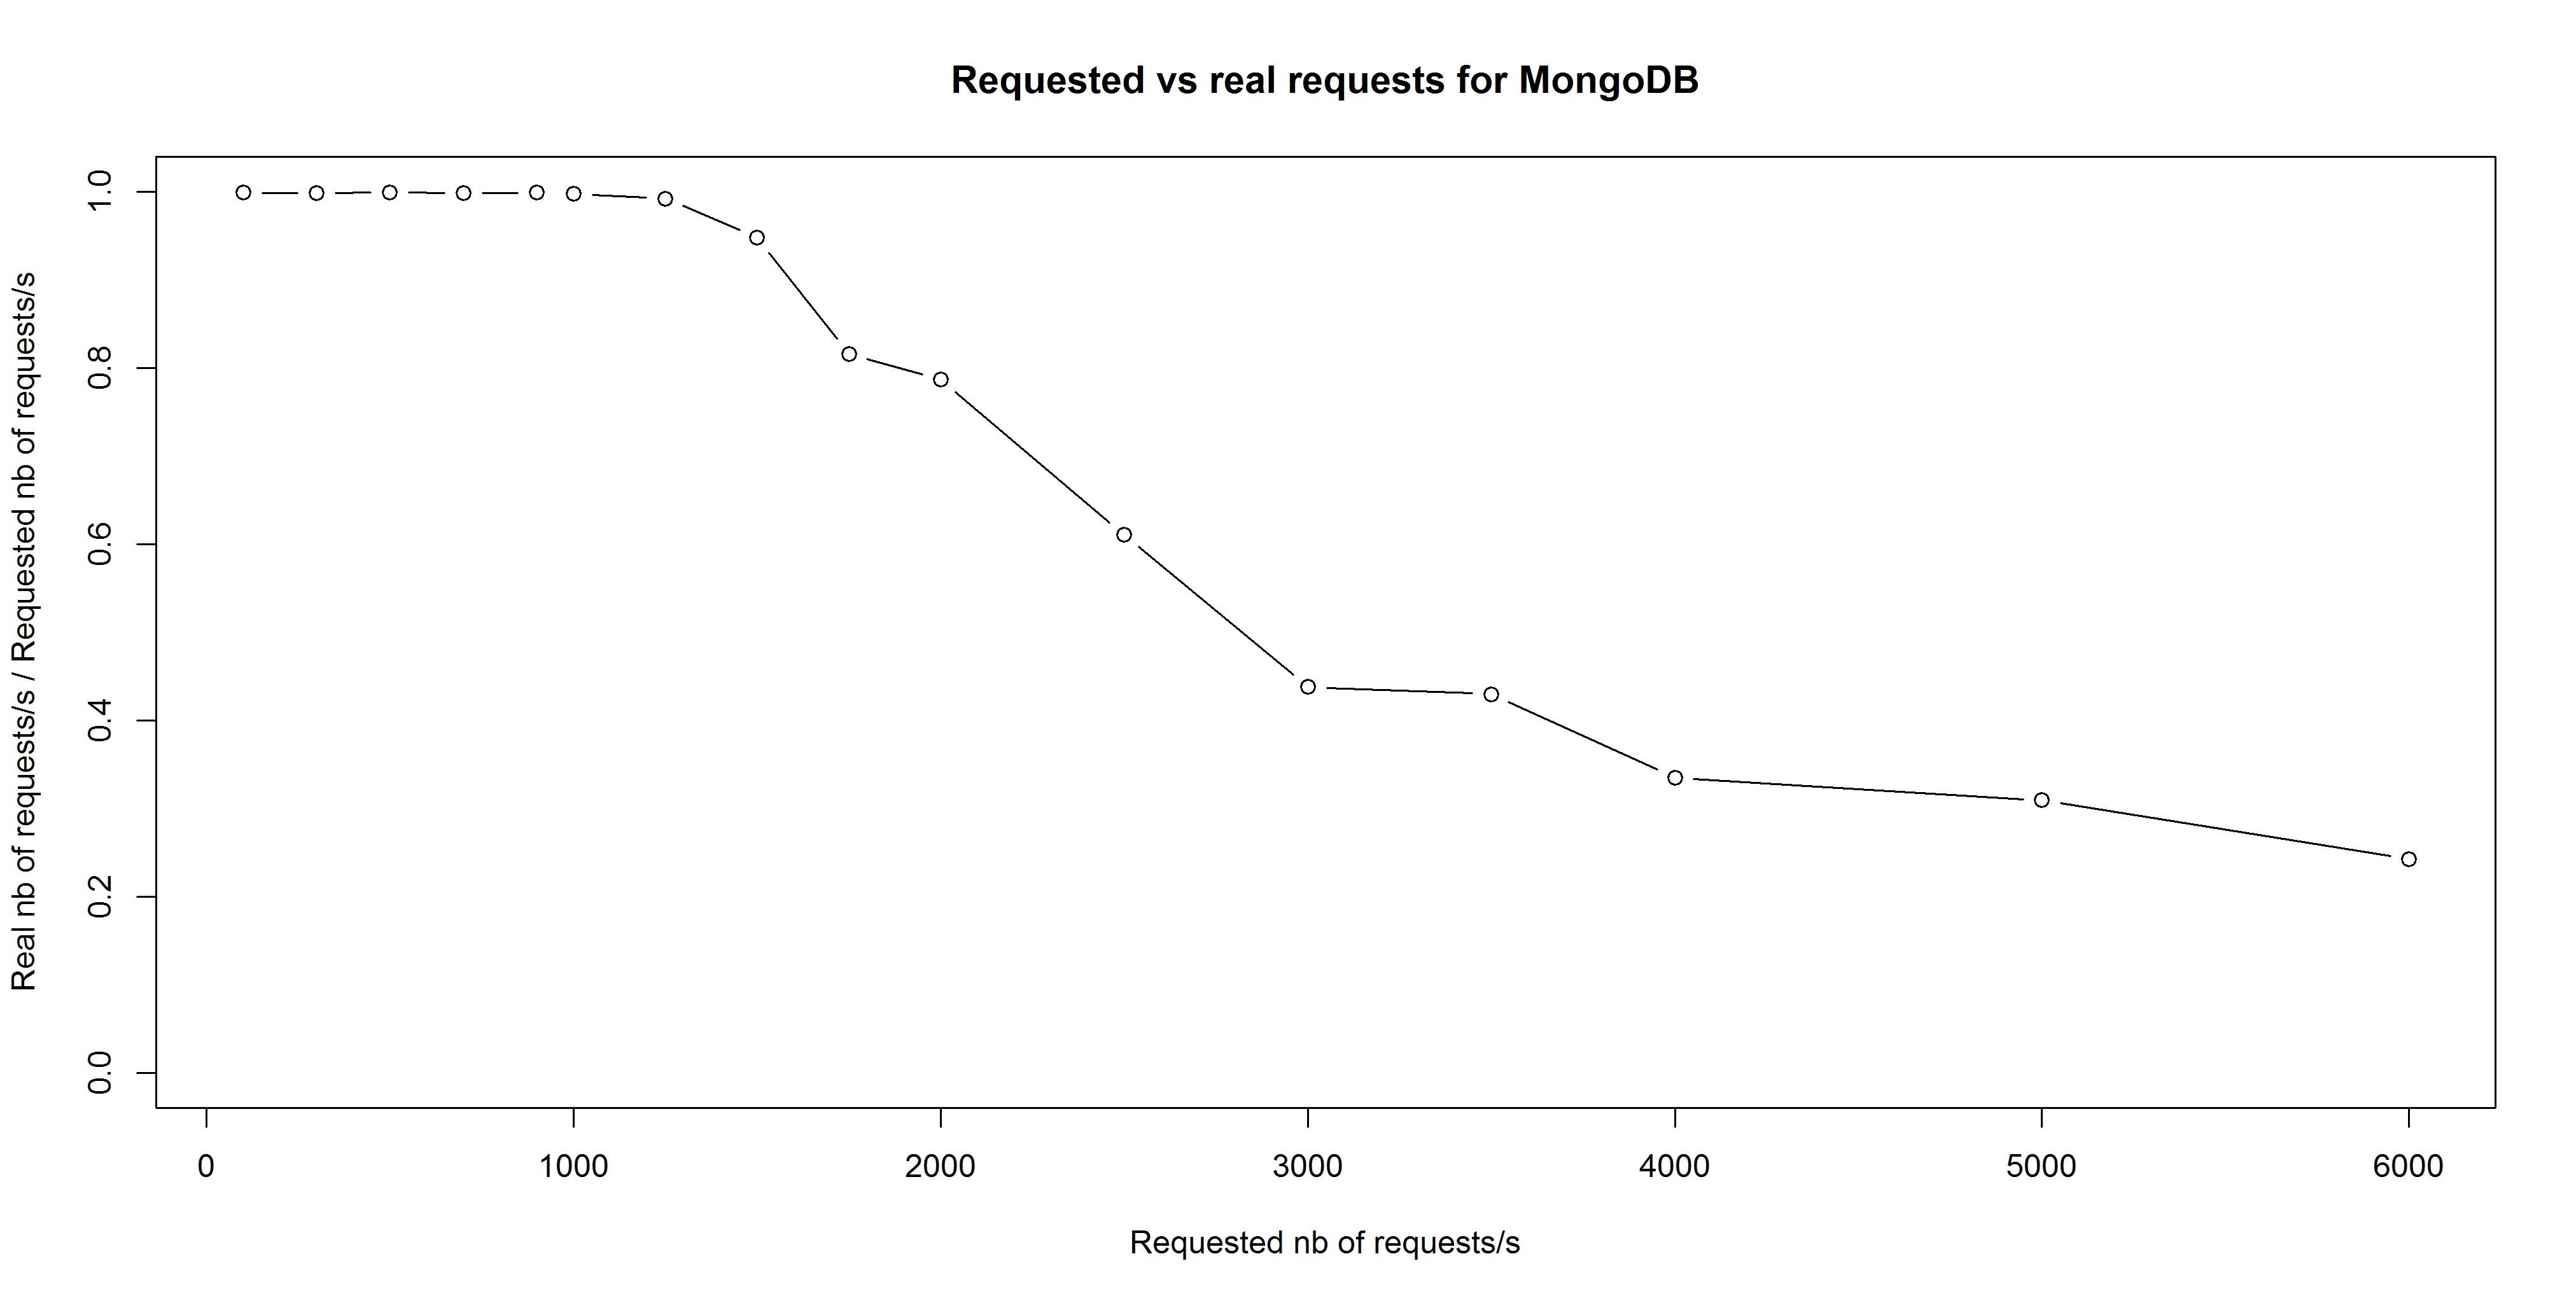
\includegraphics[width=0.95\textwidth]{img/Observaties/loadbalance-realthroughput-db-MongoDB}}
	\caption{Calibratie: Overzicht van de vertraging t.o.v. het theoretisch aantal aanvragen met een vergelijking hoeveel werkelijke aanvragen er waren voor MongoDB. }
	\label{fig:calibratie-queriesperseconde-mongodb}
\end{figure}

\begin{figure}[htb!] 
	\centering
	\subfigure{\label{fig:calibratie-queriesperseconde-pgpool-ii-1} 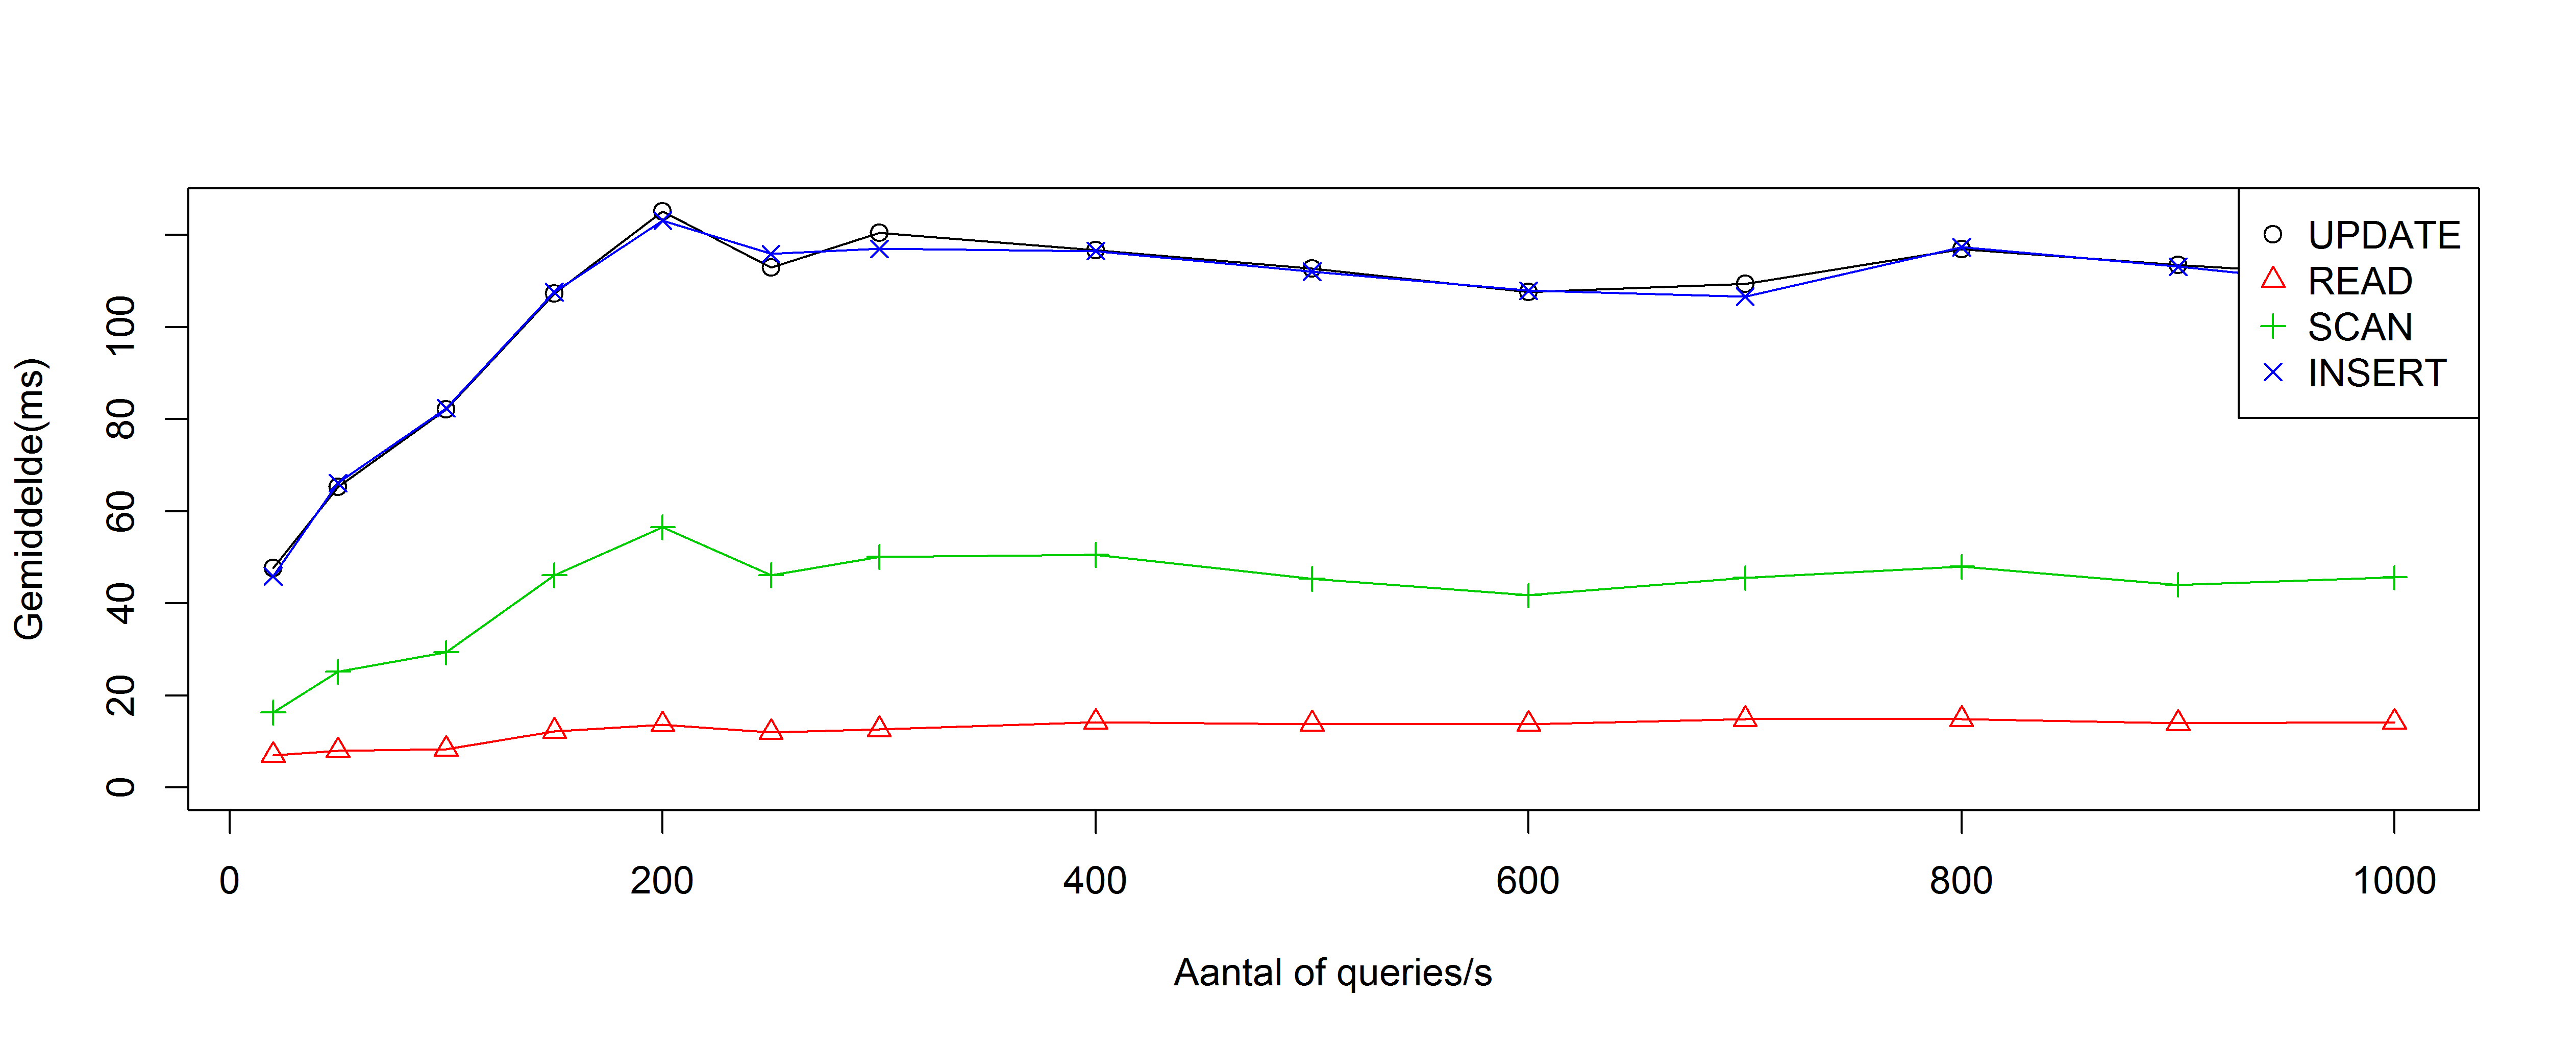
\includegraphics[width=0.95\textwidth]{img/Observaties/loadbalance-db-PostgreSQL}}
	\subfigure{\label{fig:calibratie-queriesperseconde-pgpool-ii-2} 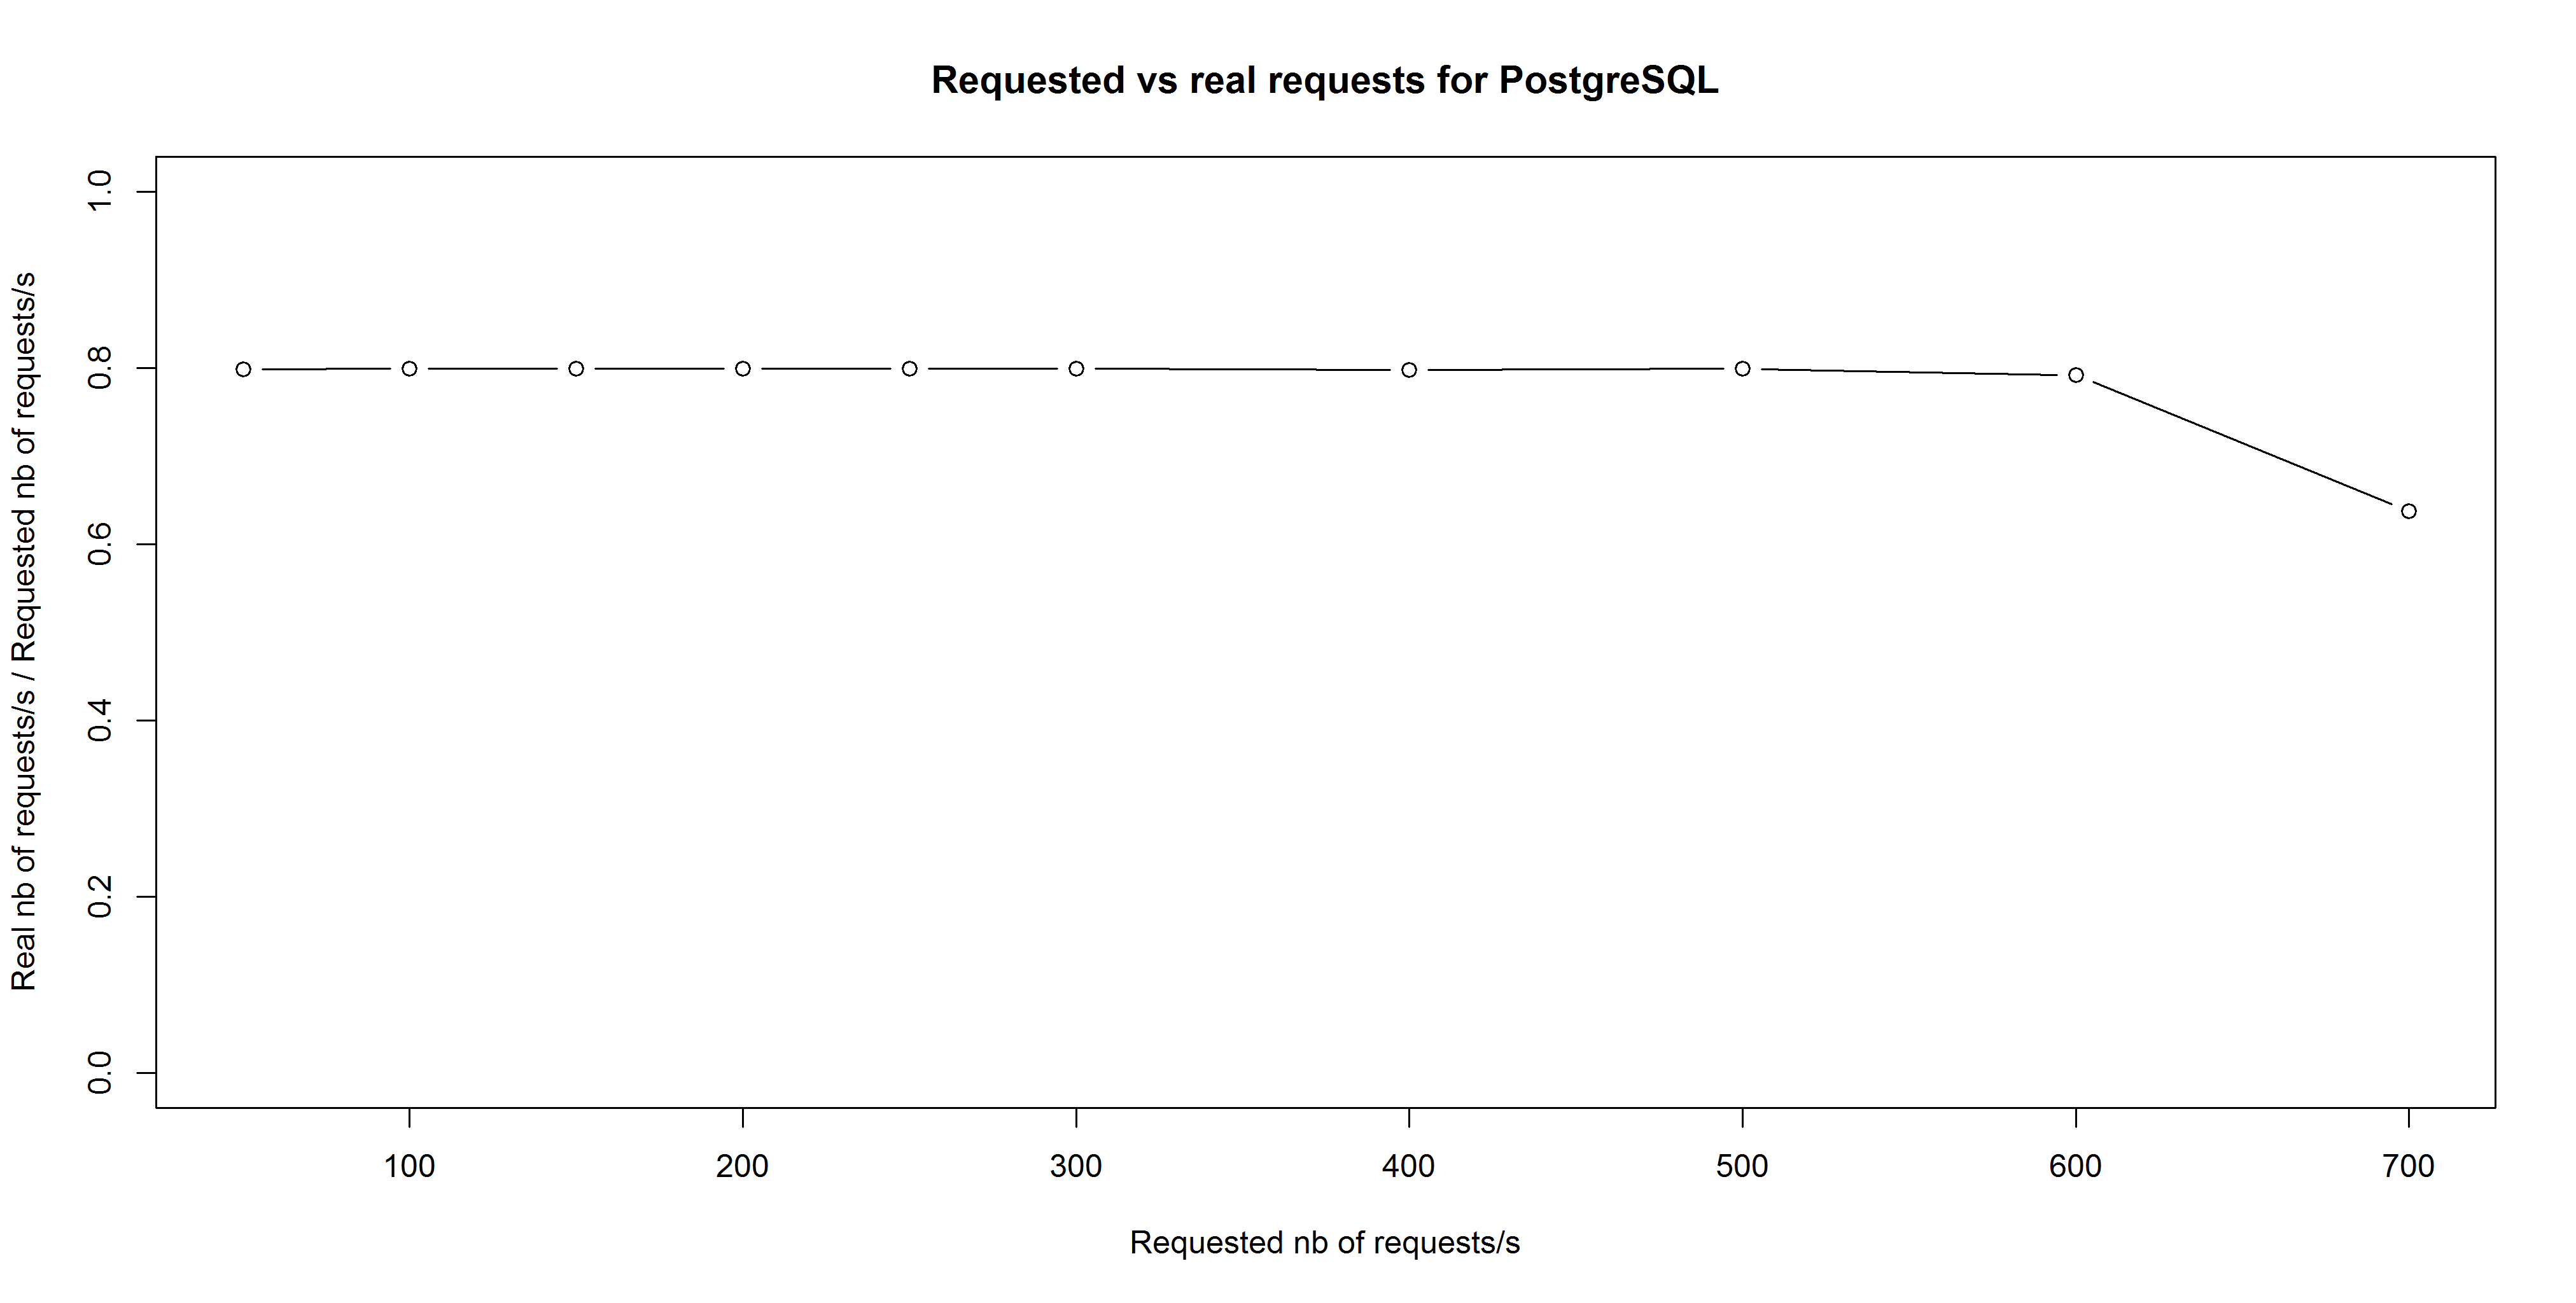
\includegraphics[width=0.95\textwidth]{img/Observaties/loadbalance-realthroughput-db-PostgreSQL}}
	\caption{Calibratie: Overzicht van de vertraging t.o.v. het theoretisch aantal aanvragen met een vergelijking hoeveel werkelijke aanvragen er waren voor Pgpool-II. }
	\label{fig:calibratie-queriesperseconde-pgpool-ii}
\end{figure}


\begin{figure}[ht!] 
	\centering
	\subfigure[Voorbeeld zacht stop]{\label{fig:beschikbaar-hbase-soft} 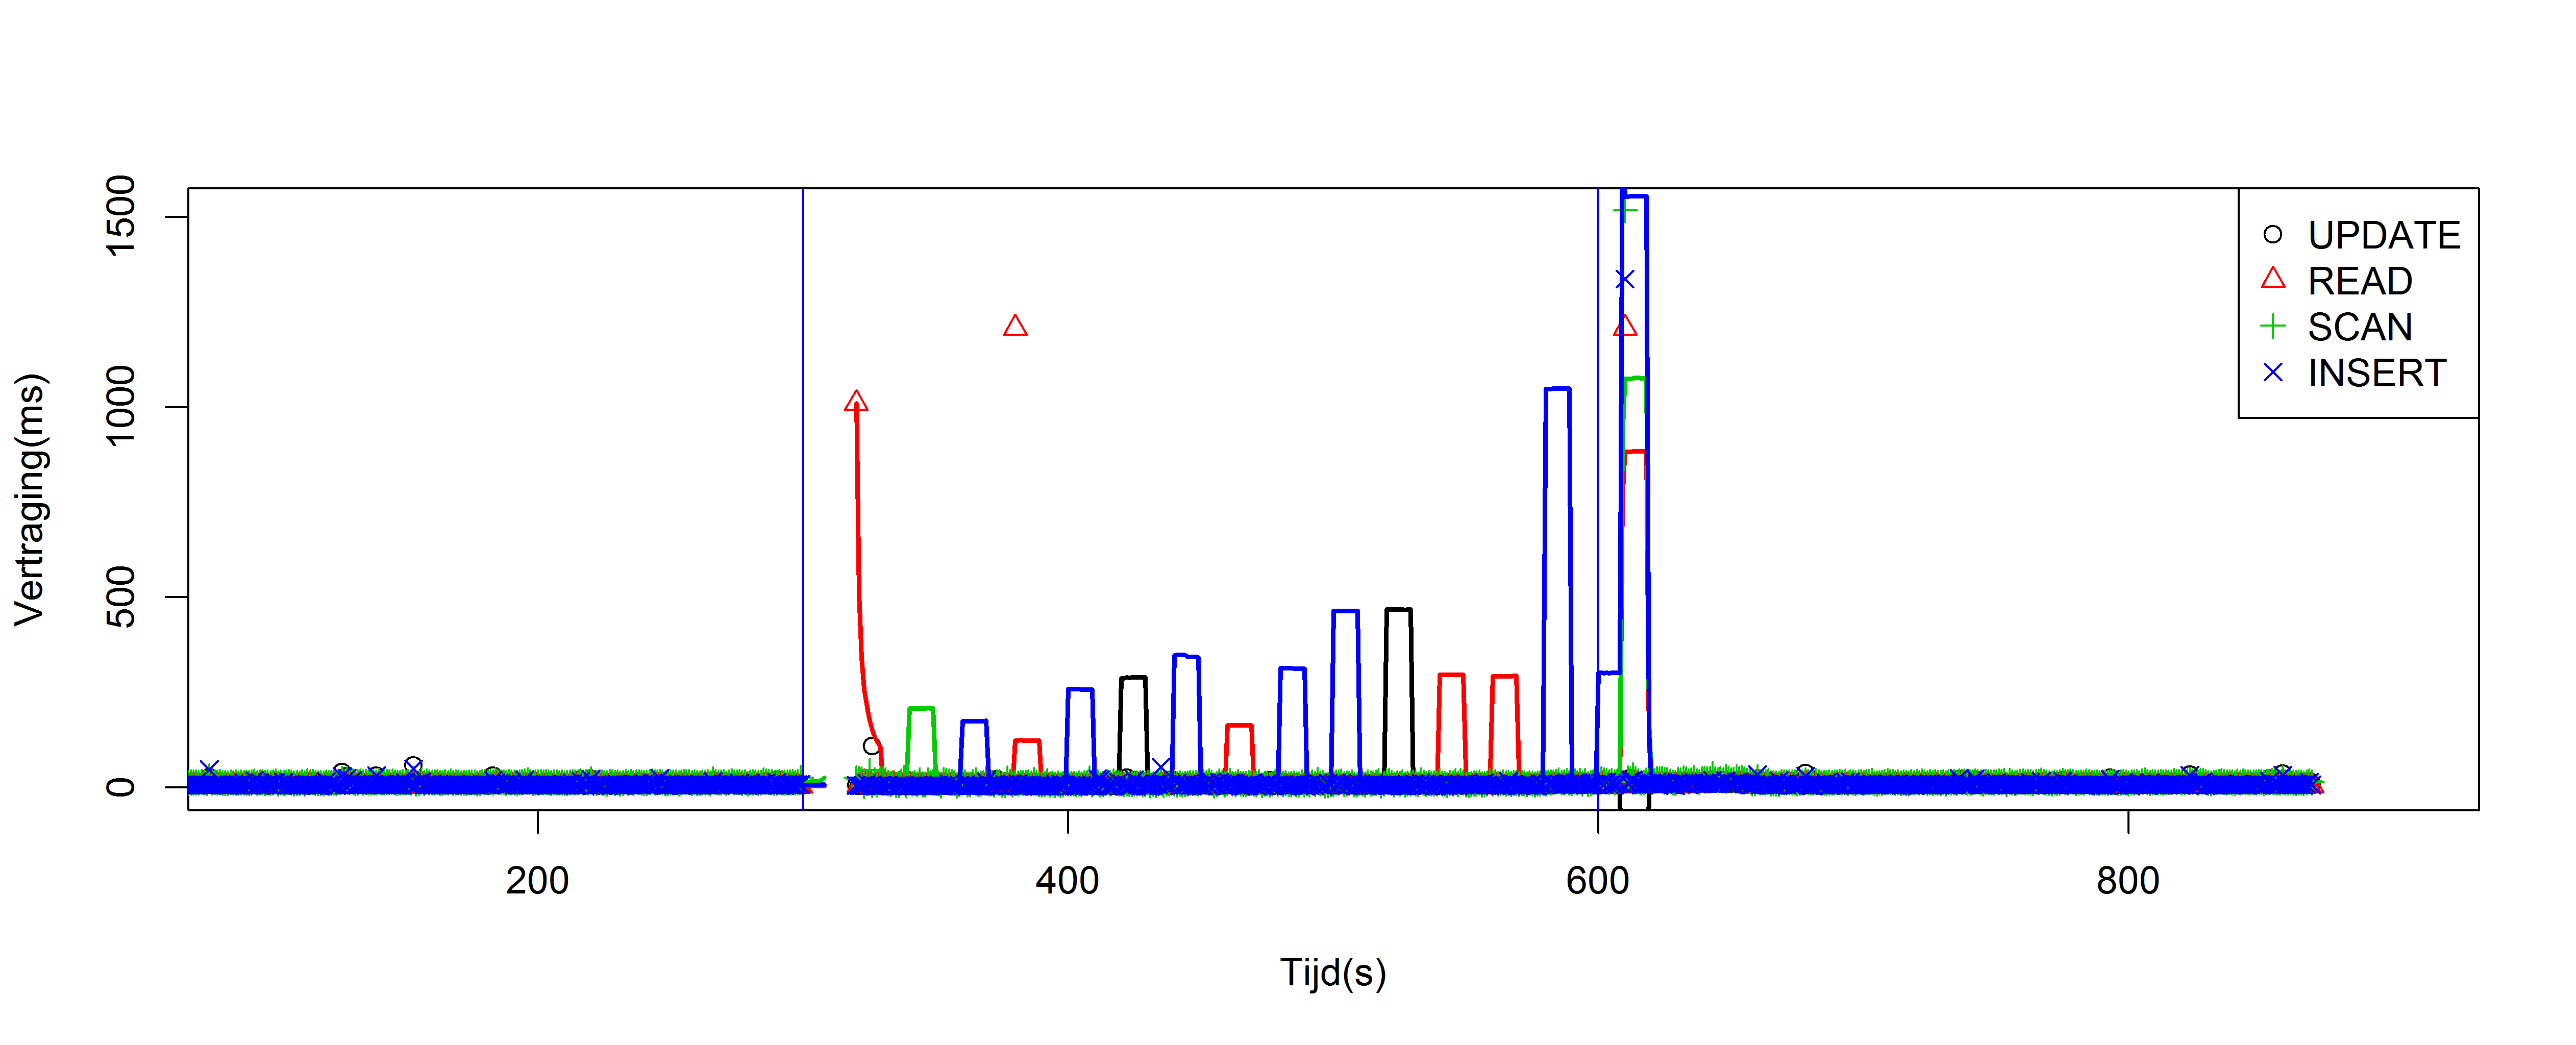
\includegraphics[width=0.95\textwidth]{img/Observaties/HBase/single-graph-2-1}}
	\subfigure[Voorbeeld netwerk onderbreking en harde stop]{\label{fig:beschikbaar-hbase-drop} 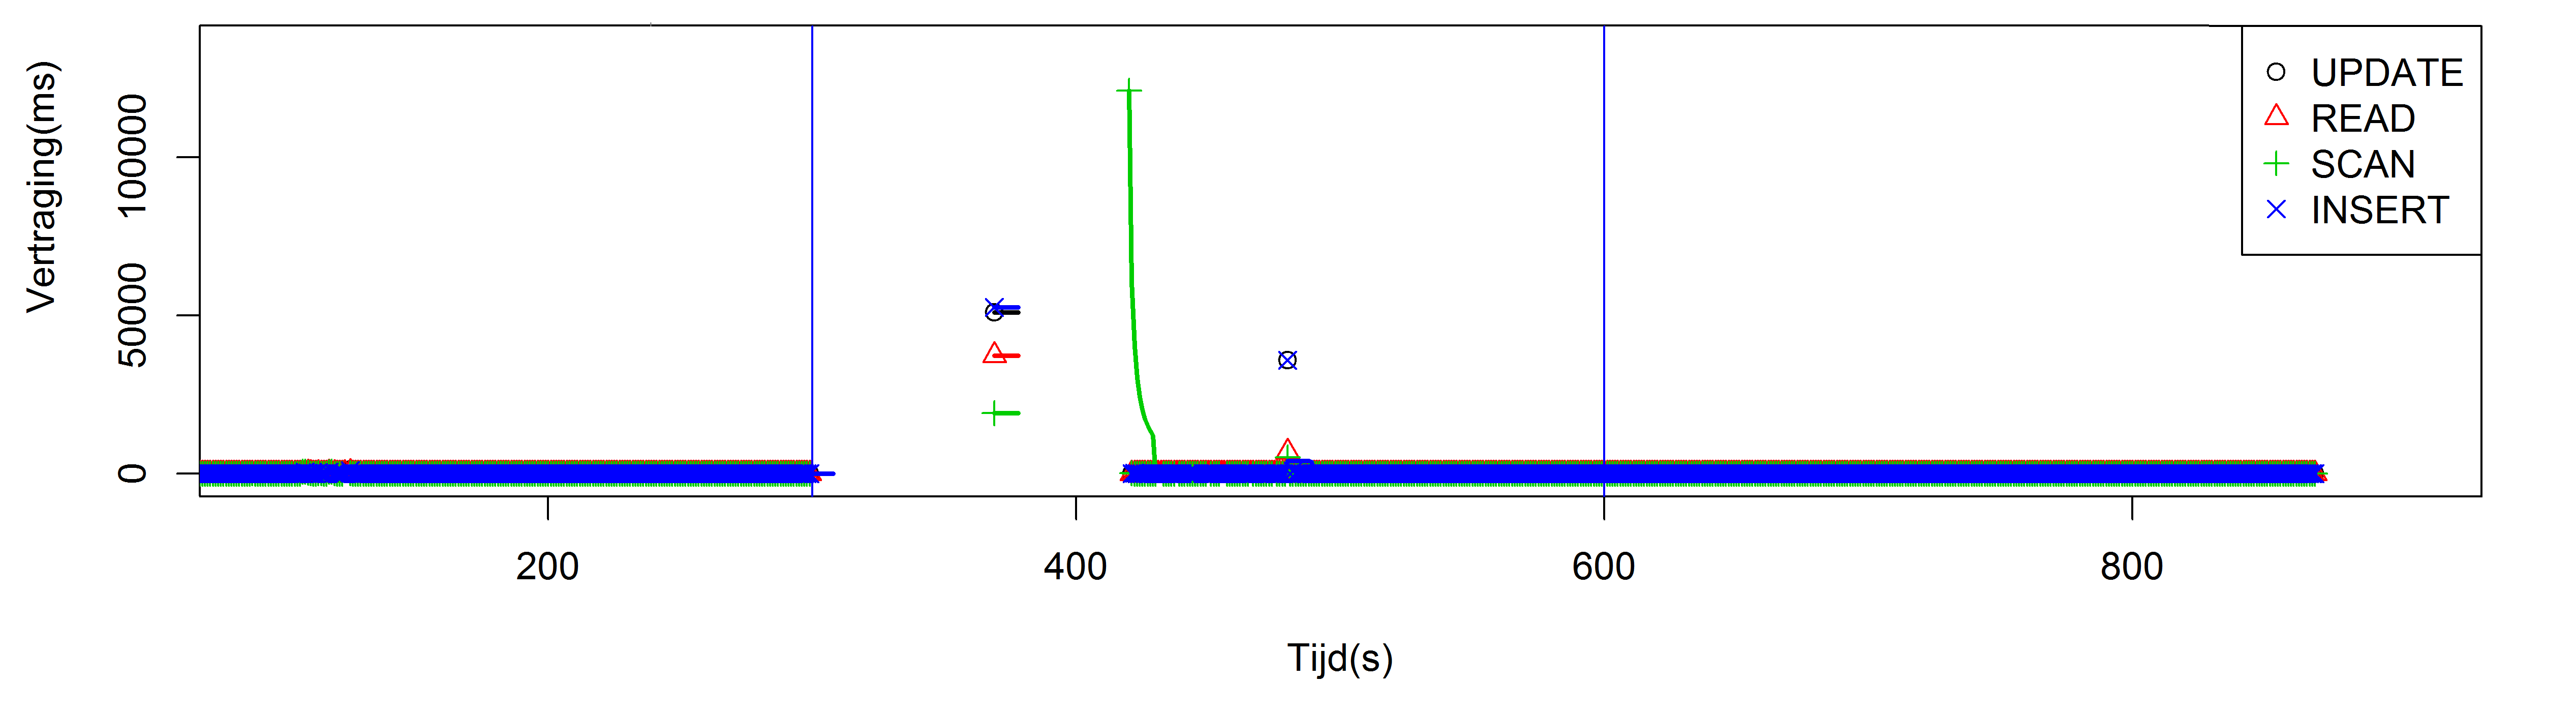
\includegraphics[width=0.95\textwidth]{img/Observaties/HBase/single-graph-2-drop-1}}
	\subfigure[Voorbeeld hard stop]{\label{fig:beschikbaar-hbase-hard} 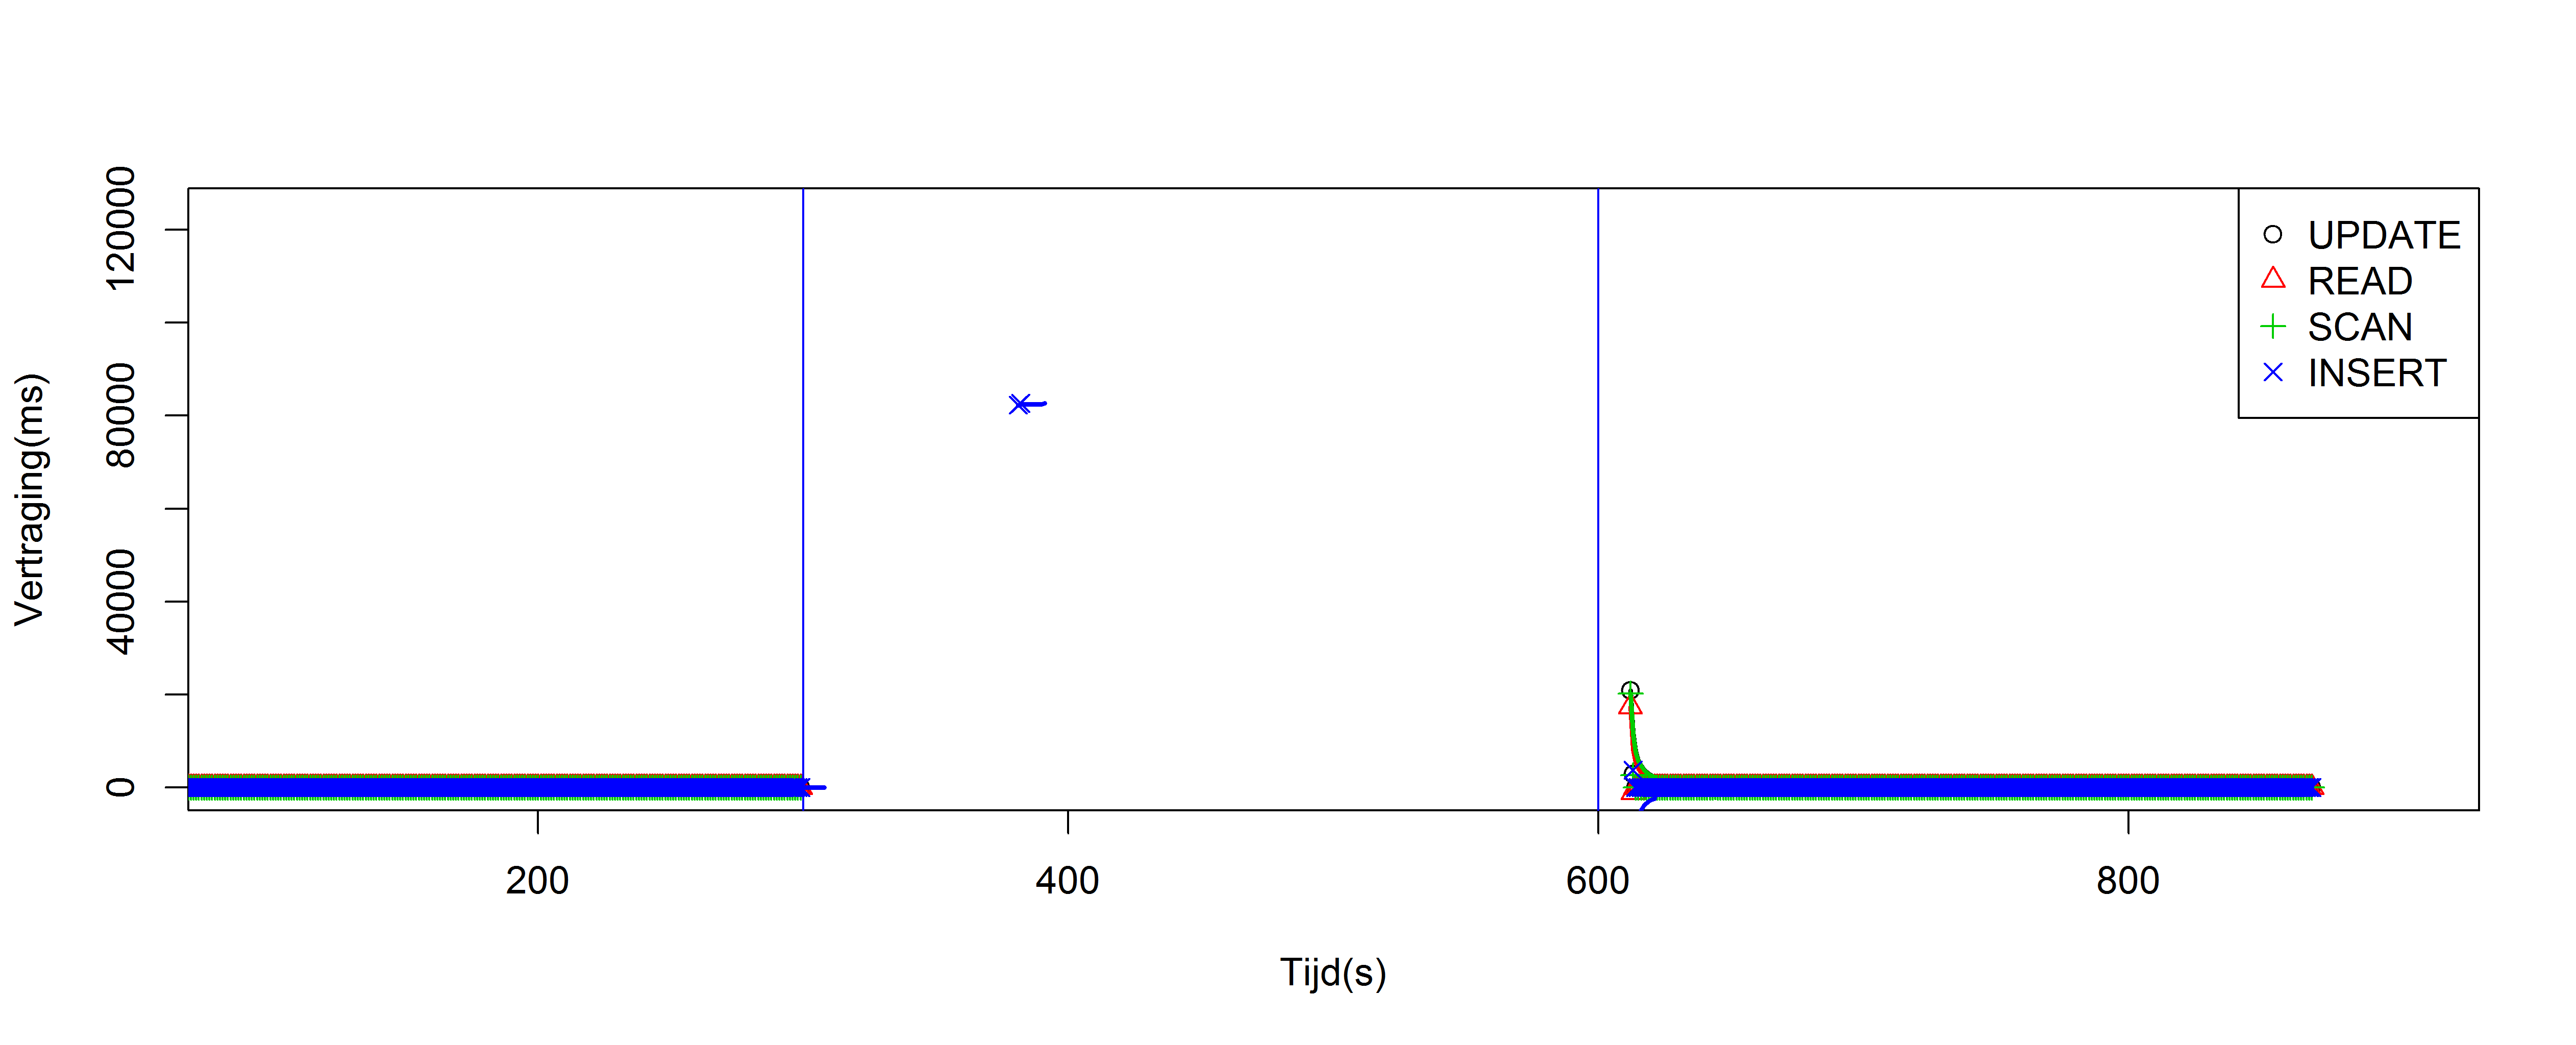
\includegraphics[width=0.95\textwidth]{img/Observaties/HBase/single-graph-3-kill-1}}
	\caption{Beschikbaarheid: Verschillende voorbeeldreacties van HBase op beschikbaarheidstesten }
	\label{fig:beschikbaar-hbase-1}
\end{figure}

\begin{figure}[ht!] 
	\centering
	\subfigure[Voorbeeld van een zacht stop, harde stop en netwerk onderbreking]{\label{fig:beschikbaar-mongodb-soft} 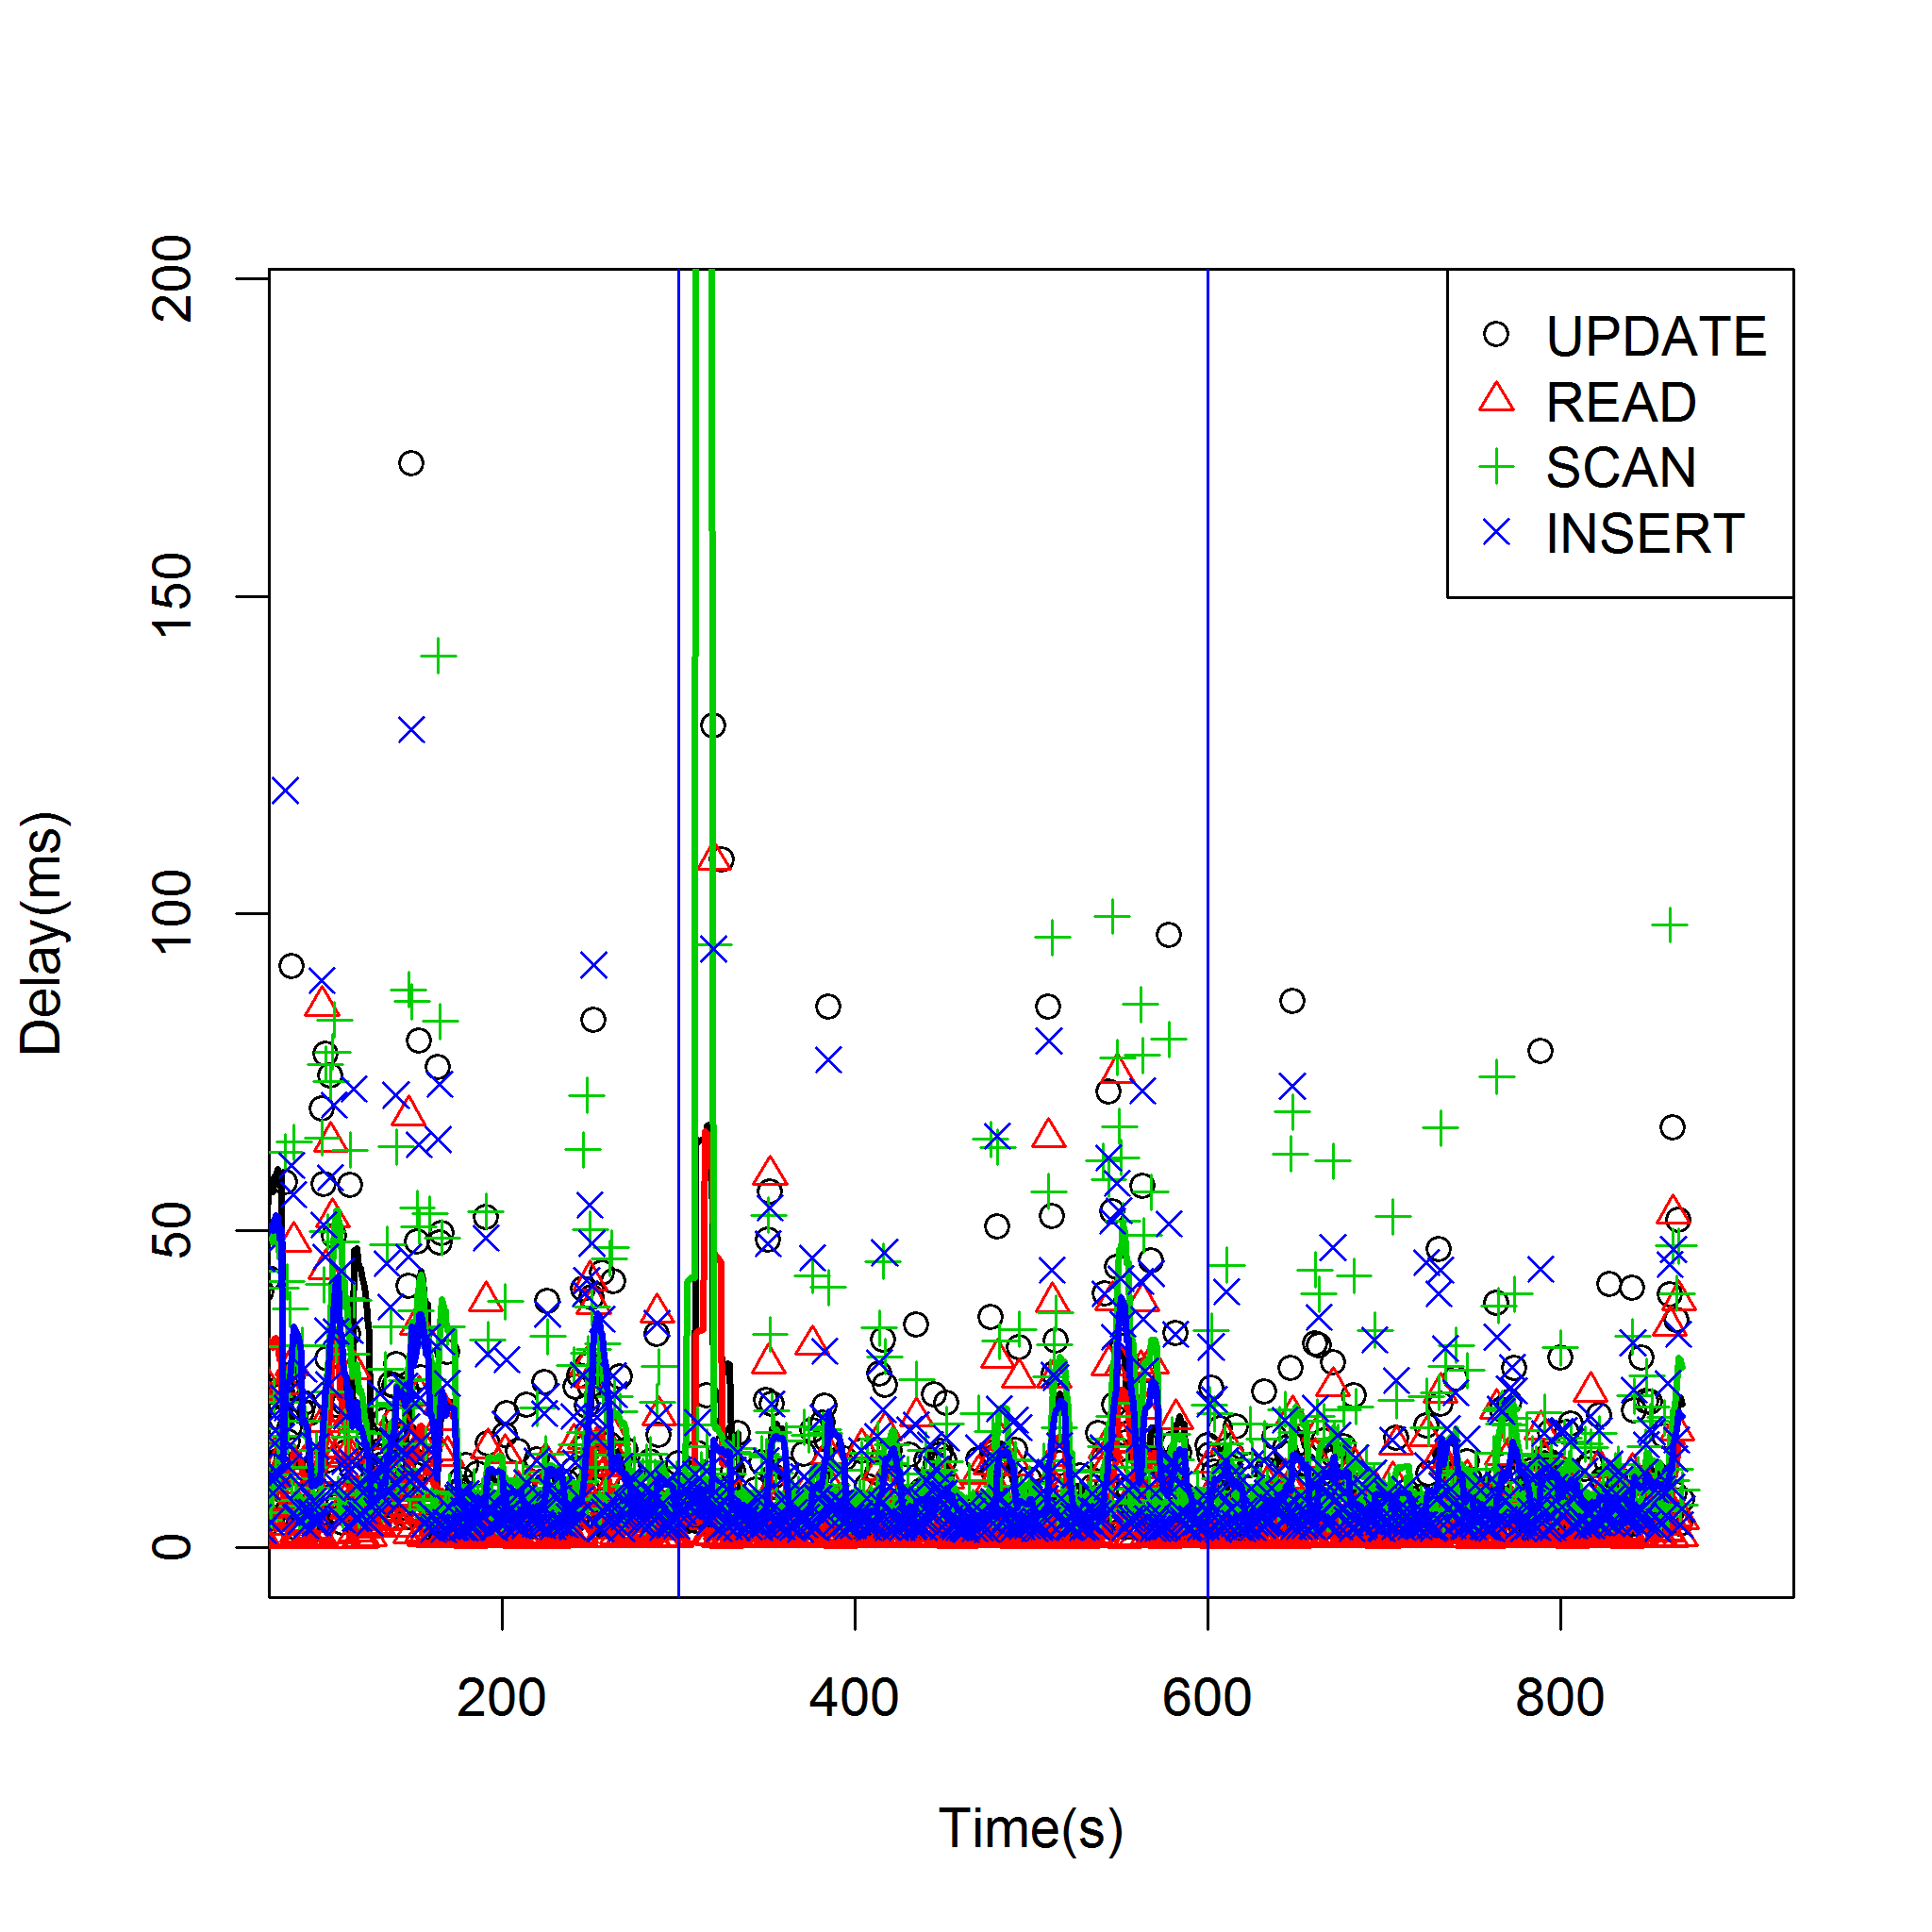
\includegraphics[width=0.95\textwidth]{img/Observaties/MongoDB/single-graph-6-1}}
	\subfigure[Zacht stop met inzoomen op het uitschakelen]{\label{fig:beschikbaar-mongodb-soft-zoom} 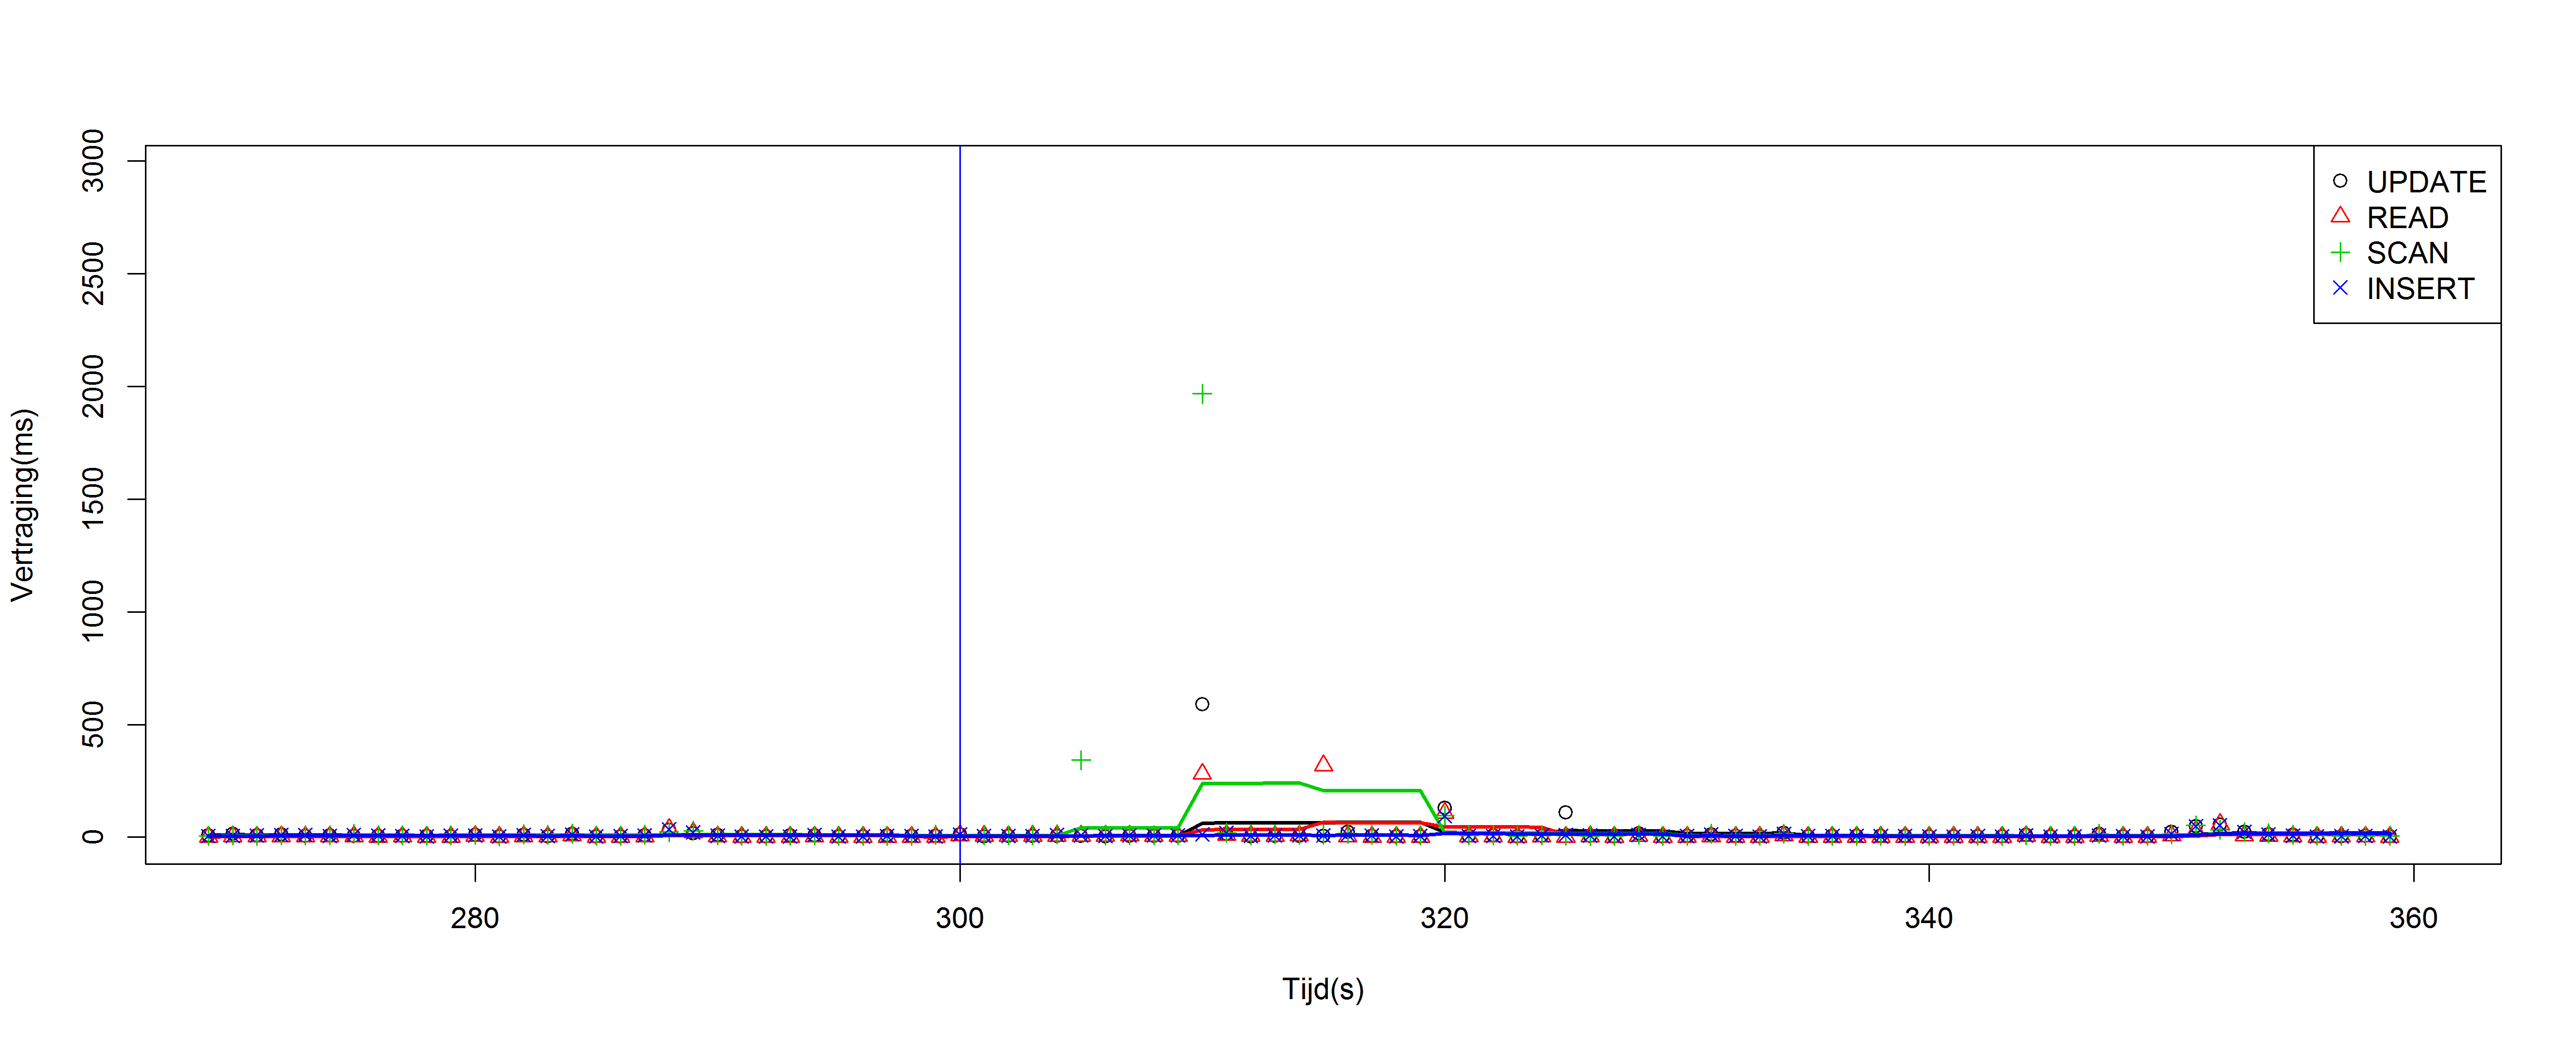
\includegraphics[width=0.95\textwidth]{img/Observaties/MongoDB/multiple-graph-interrupt-Node-6-Shut-down}}
	\subfigure[Voorbeeld netwerk onderbreking ]{\label{fig:beschikbaar-mongodb-drop} 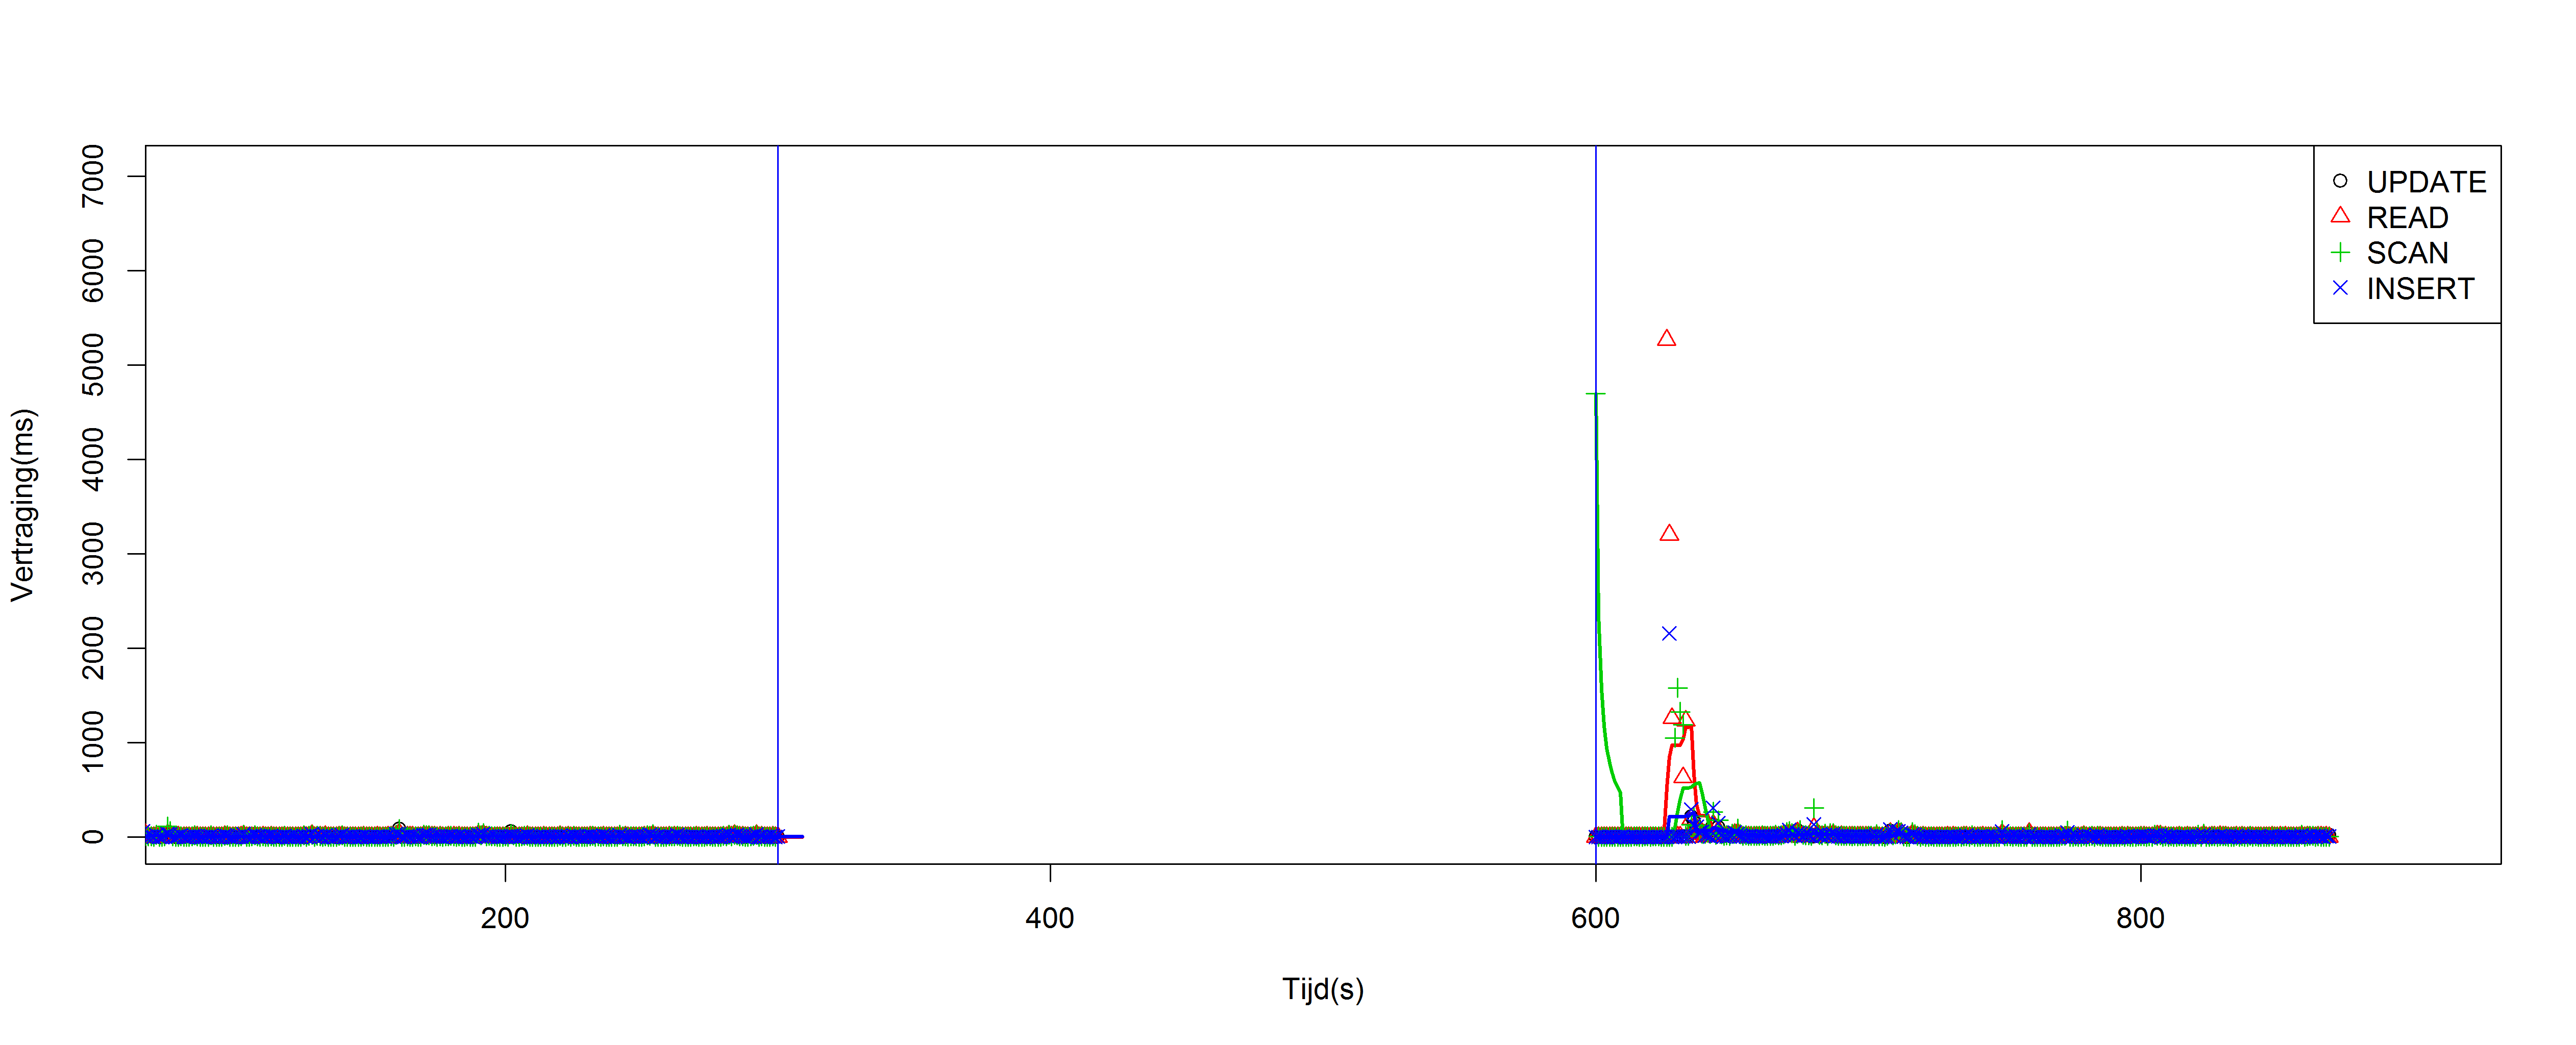
\includegraphics[width=0.95\textwidth]{img/Observaties/MongoDB/single-graph-4-drop-1}}
	\caption{Beschikbaarheid: Verschillende voorbeeldreacties van MongoDB op beschikbaarheidstesten }
	\label{fig:beschikbaar-mongodb-1}
\end{figure}

\begin{figure}[ht!] 
	\centering
	\subfigure[Voorbeeld van een zacht stop]{\label{fig:beschikbaar-pgpool-soft} 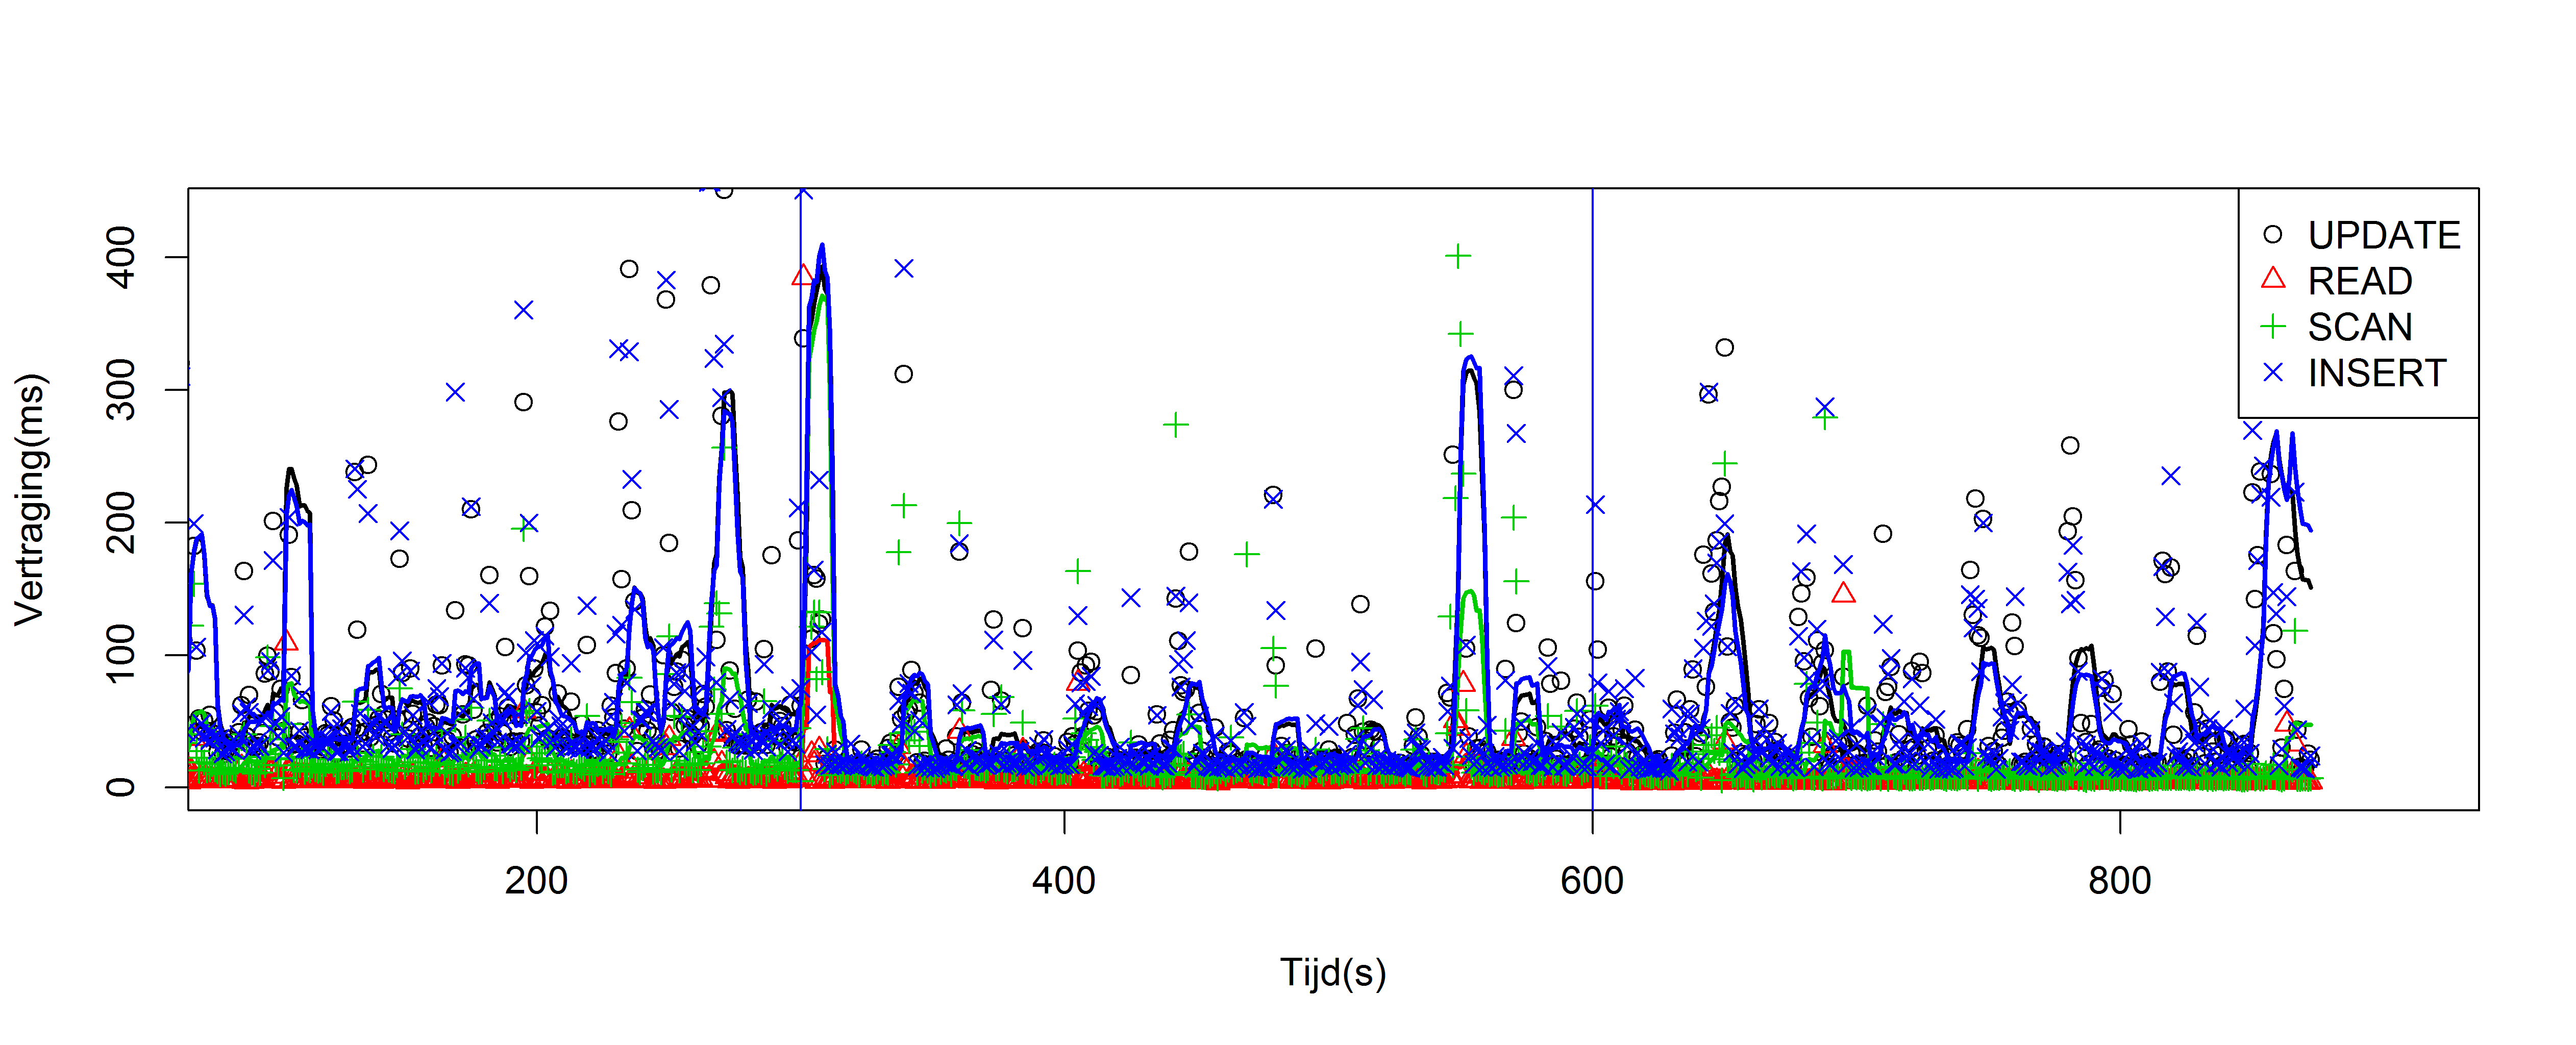
\includegraphics[width=0.95\textwidth]{img/Observaties/Pgpool/single-graph-1-2}}
	\subfigure[Voorbeeld van een harde stop of netwerk onderbreking]{\label{fig:beschikbaar-pgpool-netwerk} 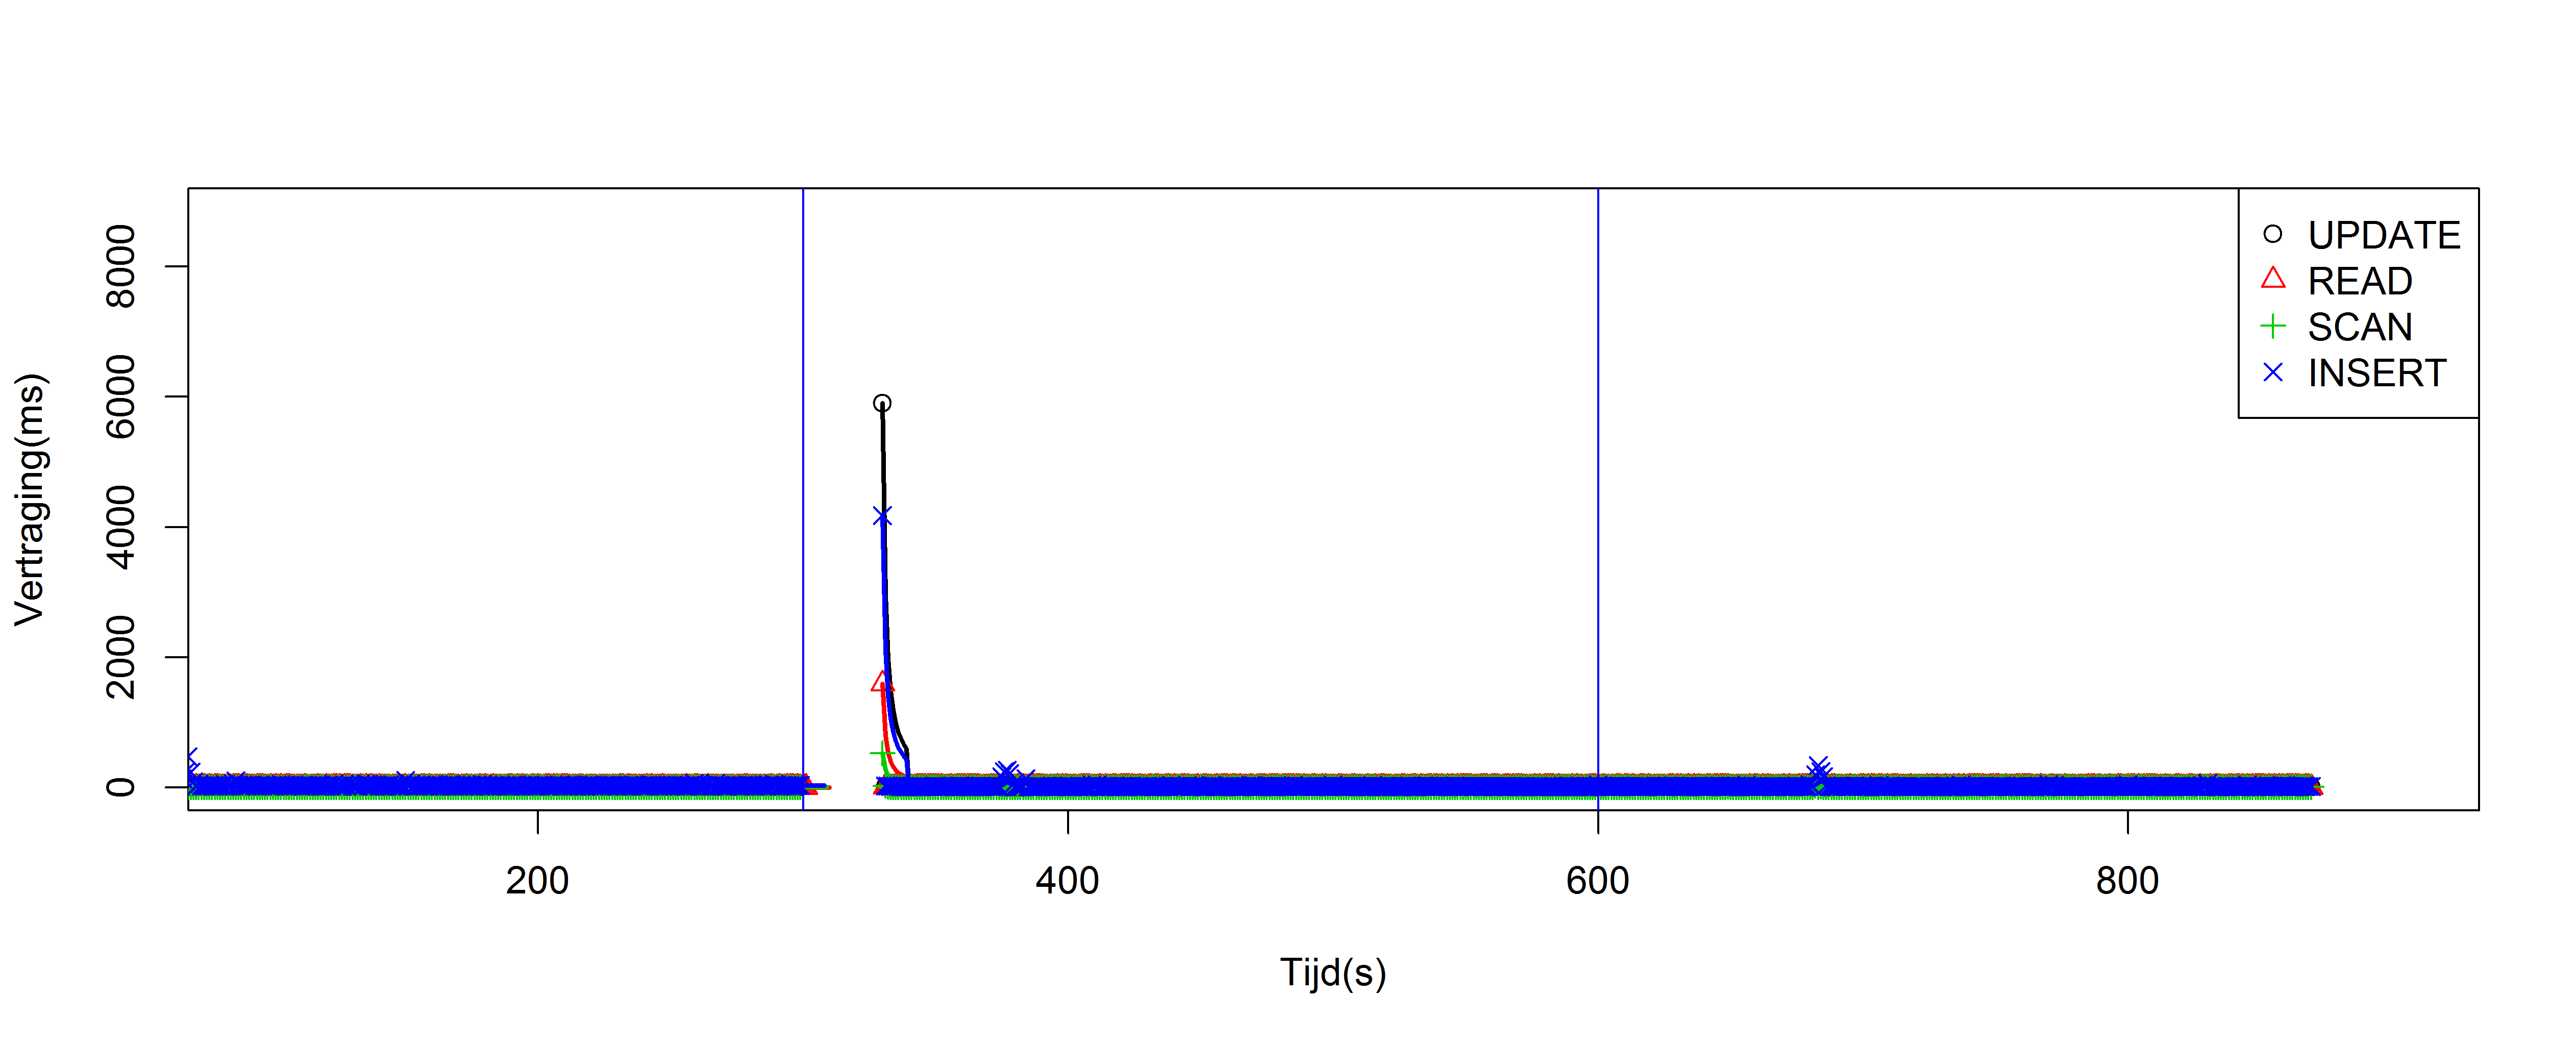
\includegraphics[width=0.95\textwidth]{img/Observaties/Pgpool/single-graph-1-drop-1}}
	\subfigure[Boxplot met leesvertragingen]{\label{fig:beschikbaar-pgpool-boxplot-read} 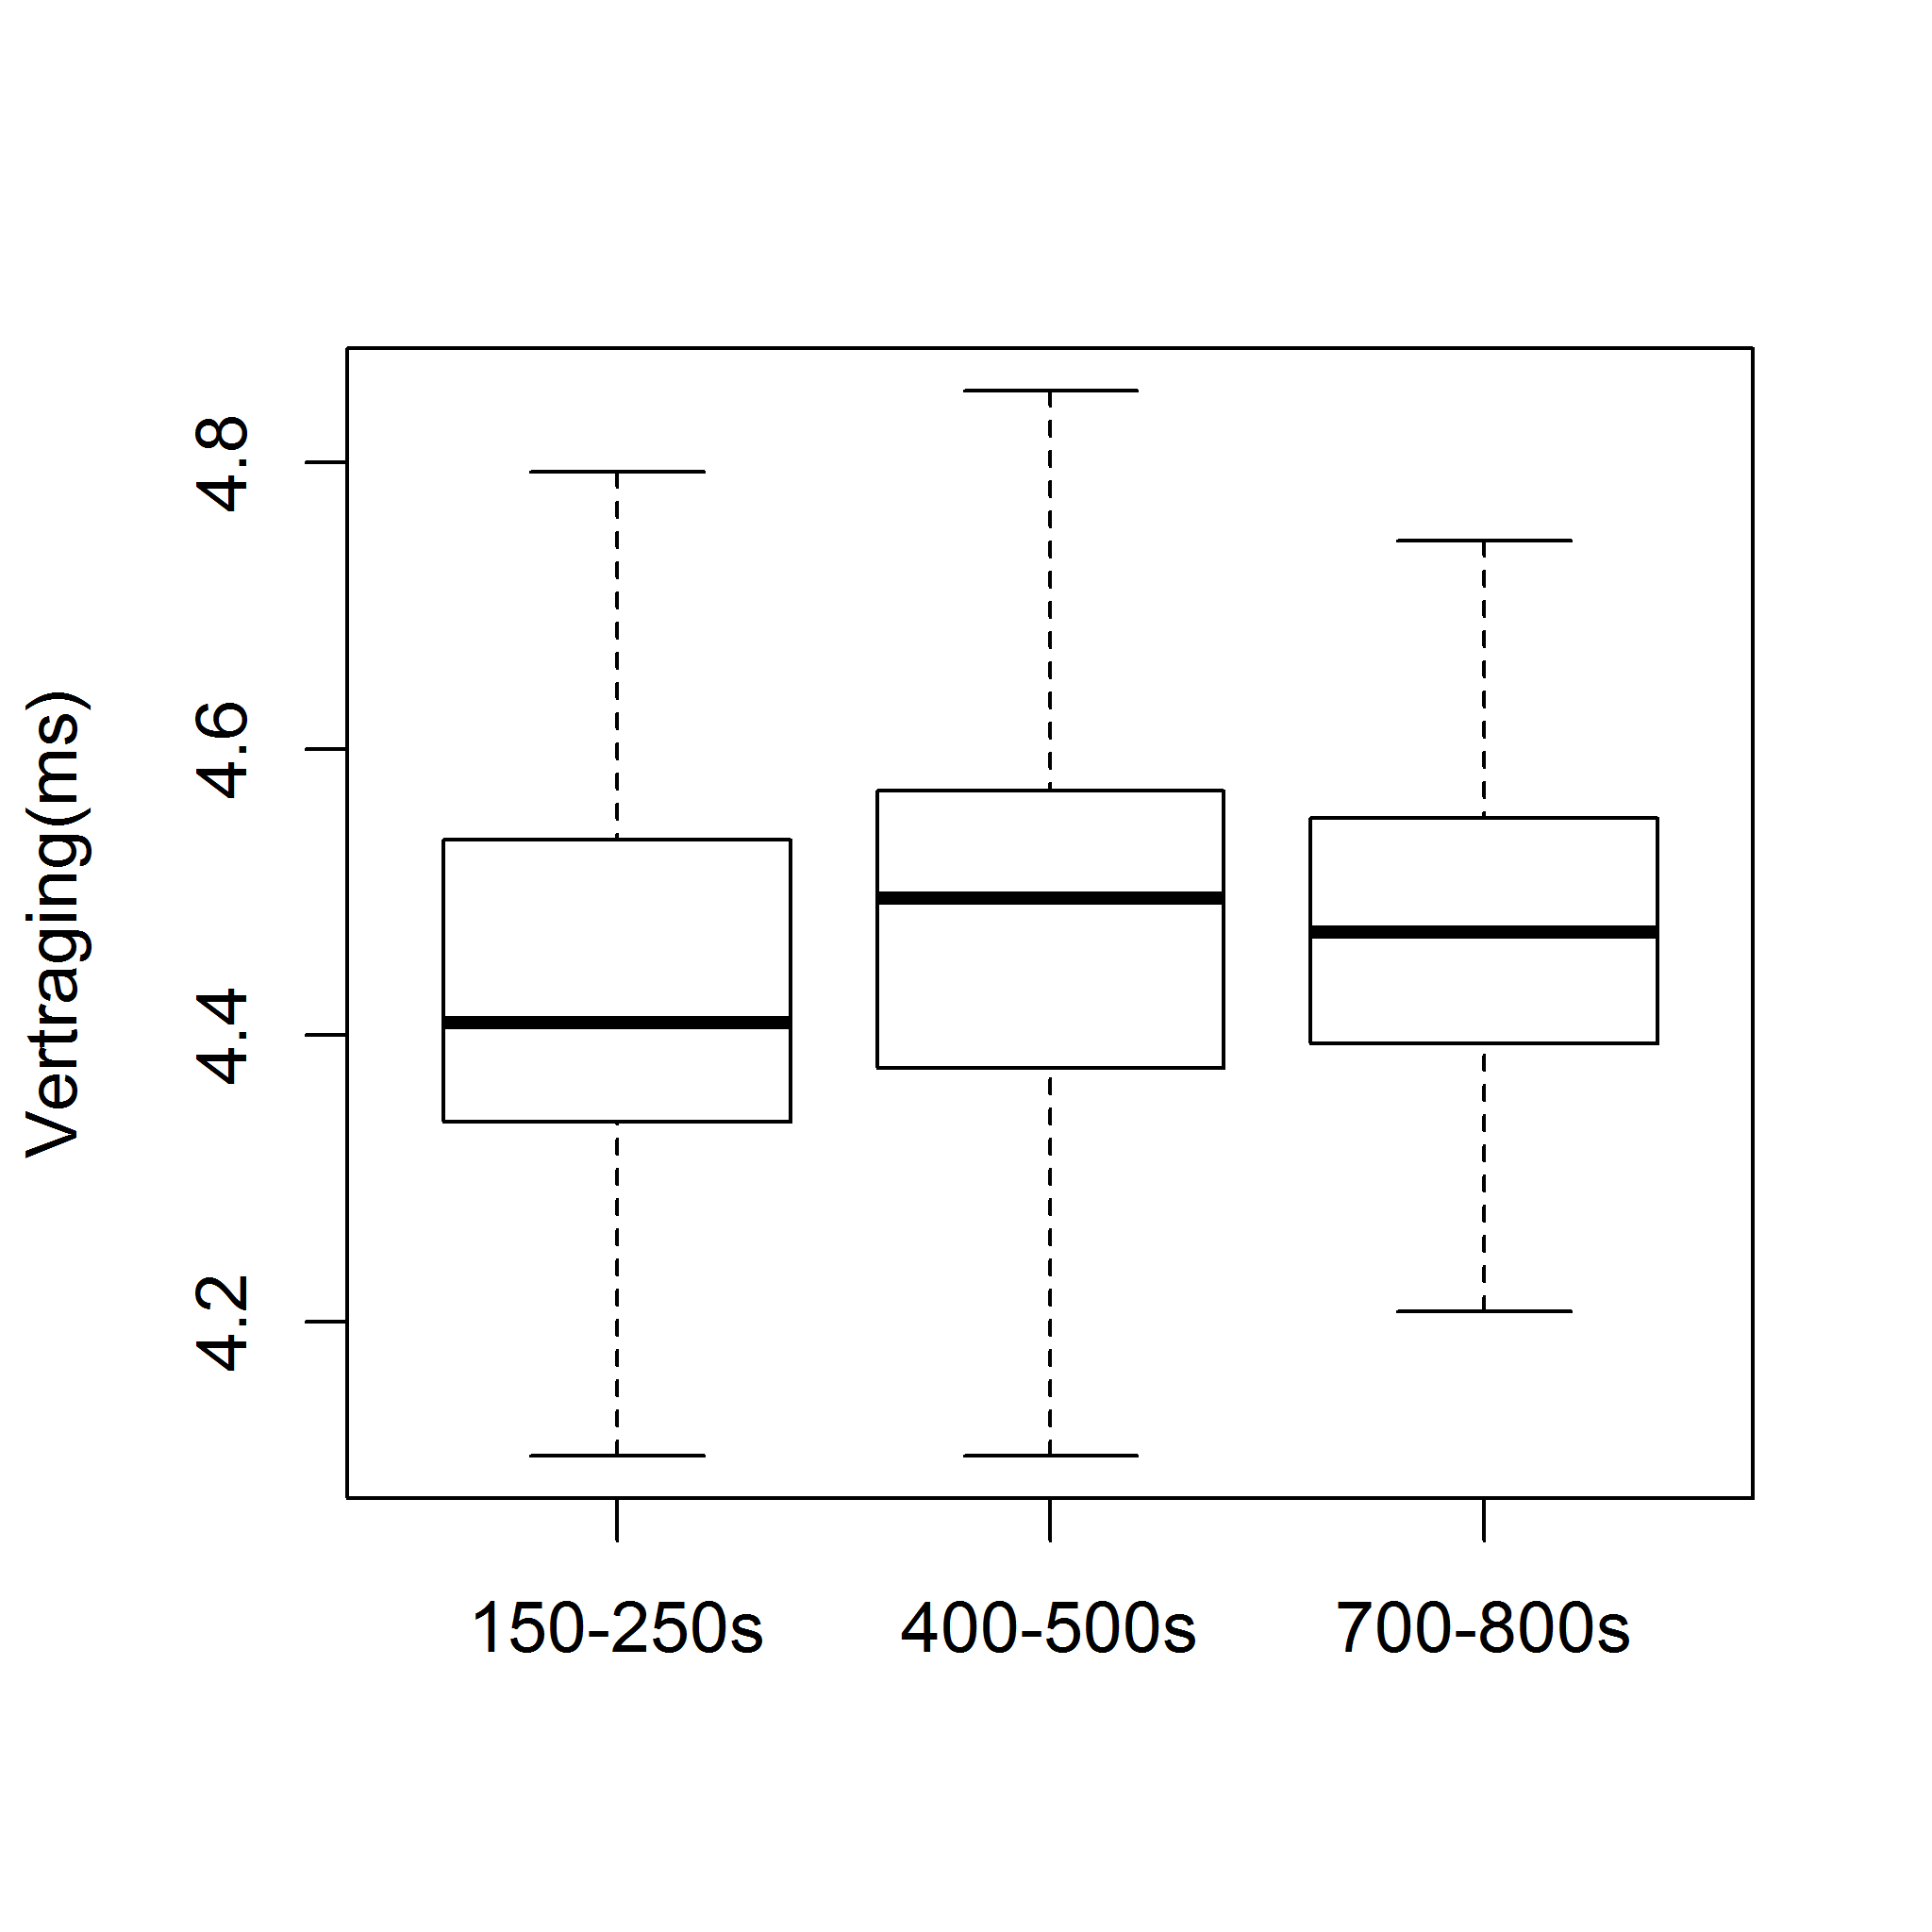
\includegraphics[width=0.45\textwidth]{img/Observaties/Pgpool/boxplot-graph-Node-1-READ}}
	\subfigure[Boxplot met schrijf vertragingen]{\label{fig:beschikbaar-pgpool-boxplot-write} 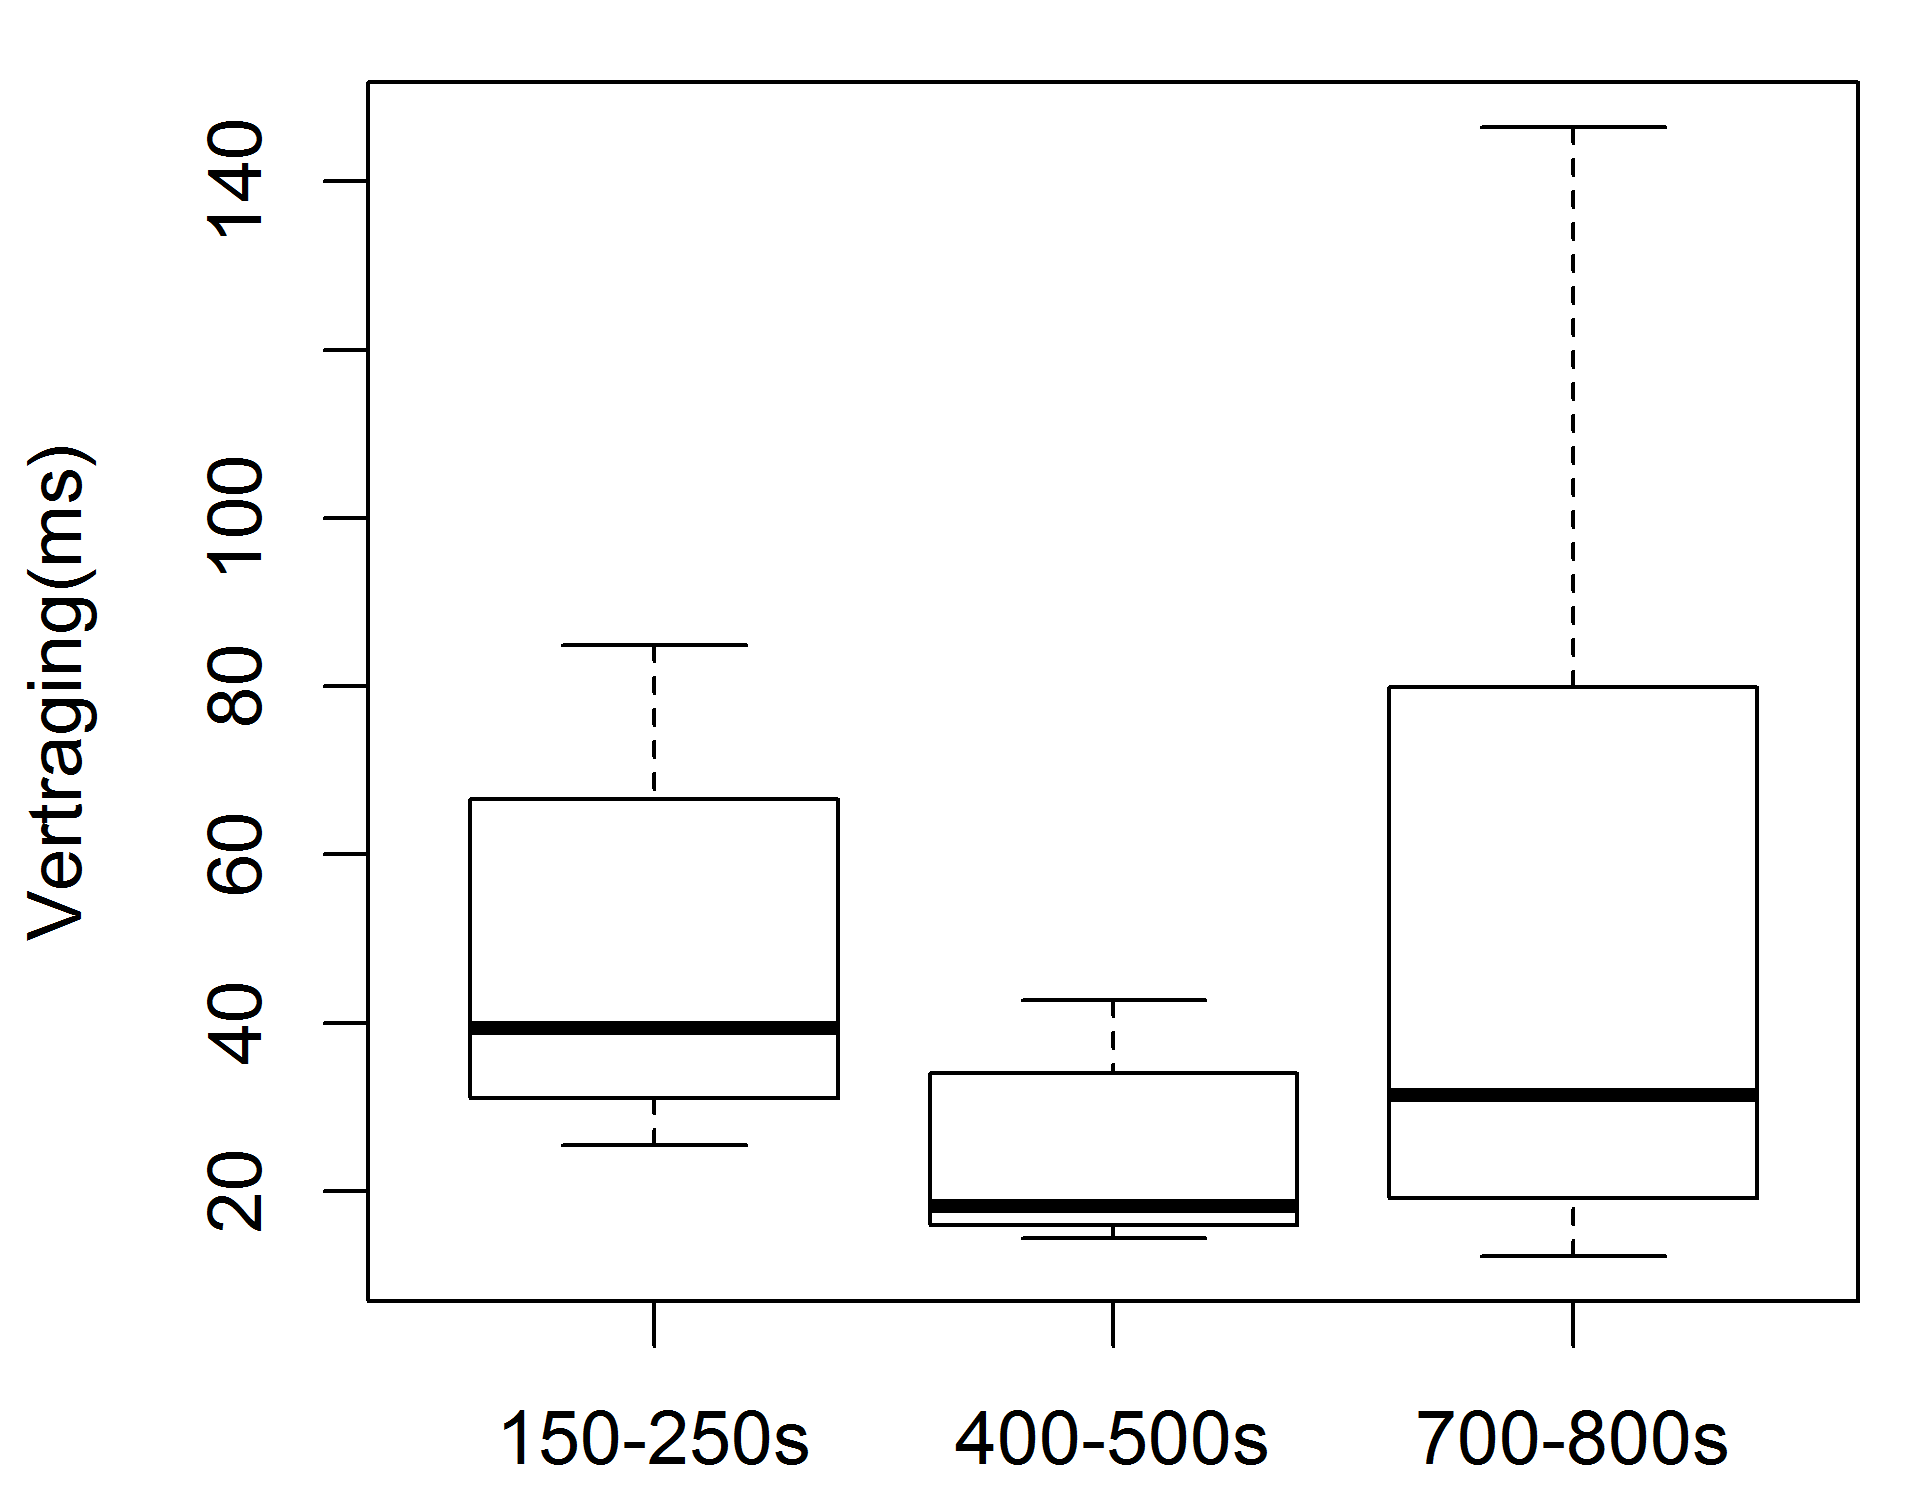
\includegraphics[width=0.45\textwidth]{img/Observaties/Pgpool/boxplot-graph-Node-1-UPDATE}}
	\caption{Beschikbaarheid: Verschillende voorbeeldreacties van Pgpool-II op beschikbaarheidstesten }
	\label{fig:beschikbaar-pgpool}
\end{figure}

\begin{figure}[ht!] 
	\centering
	\subfigure[Starttijdstippen van verschillende lezers voor lezen van consistente data]{\label{fig:consistentie-hbase-start} 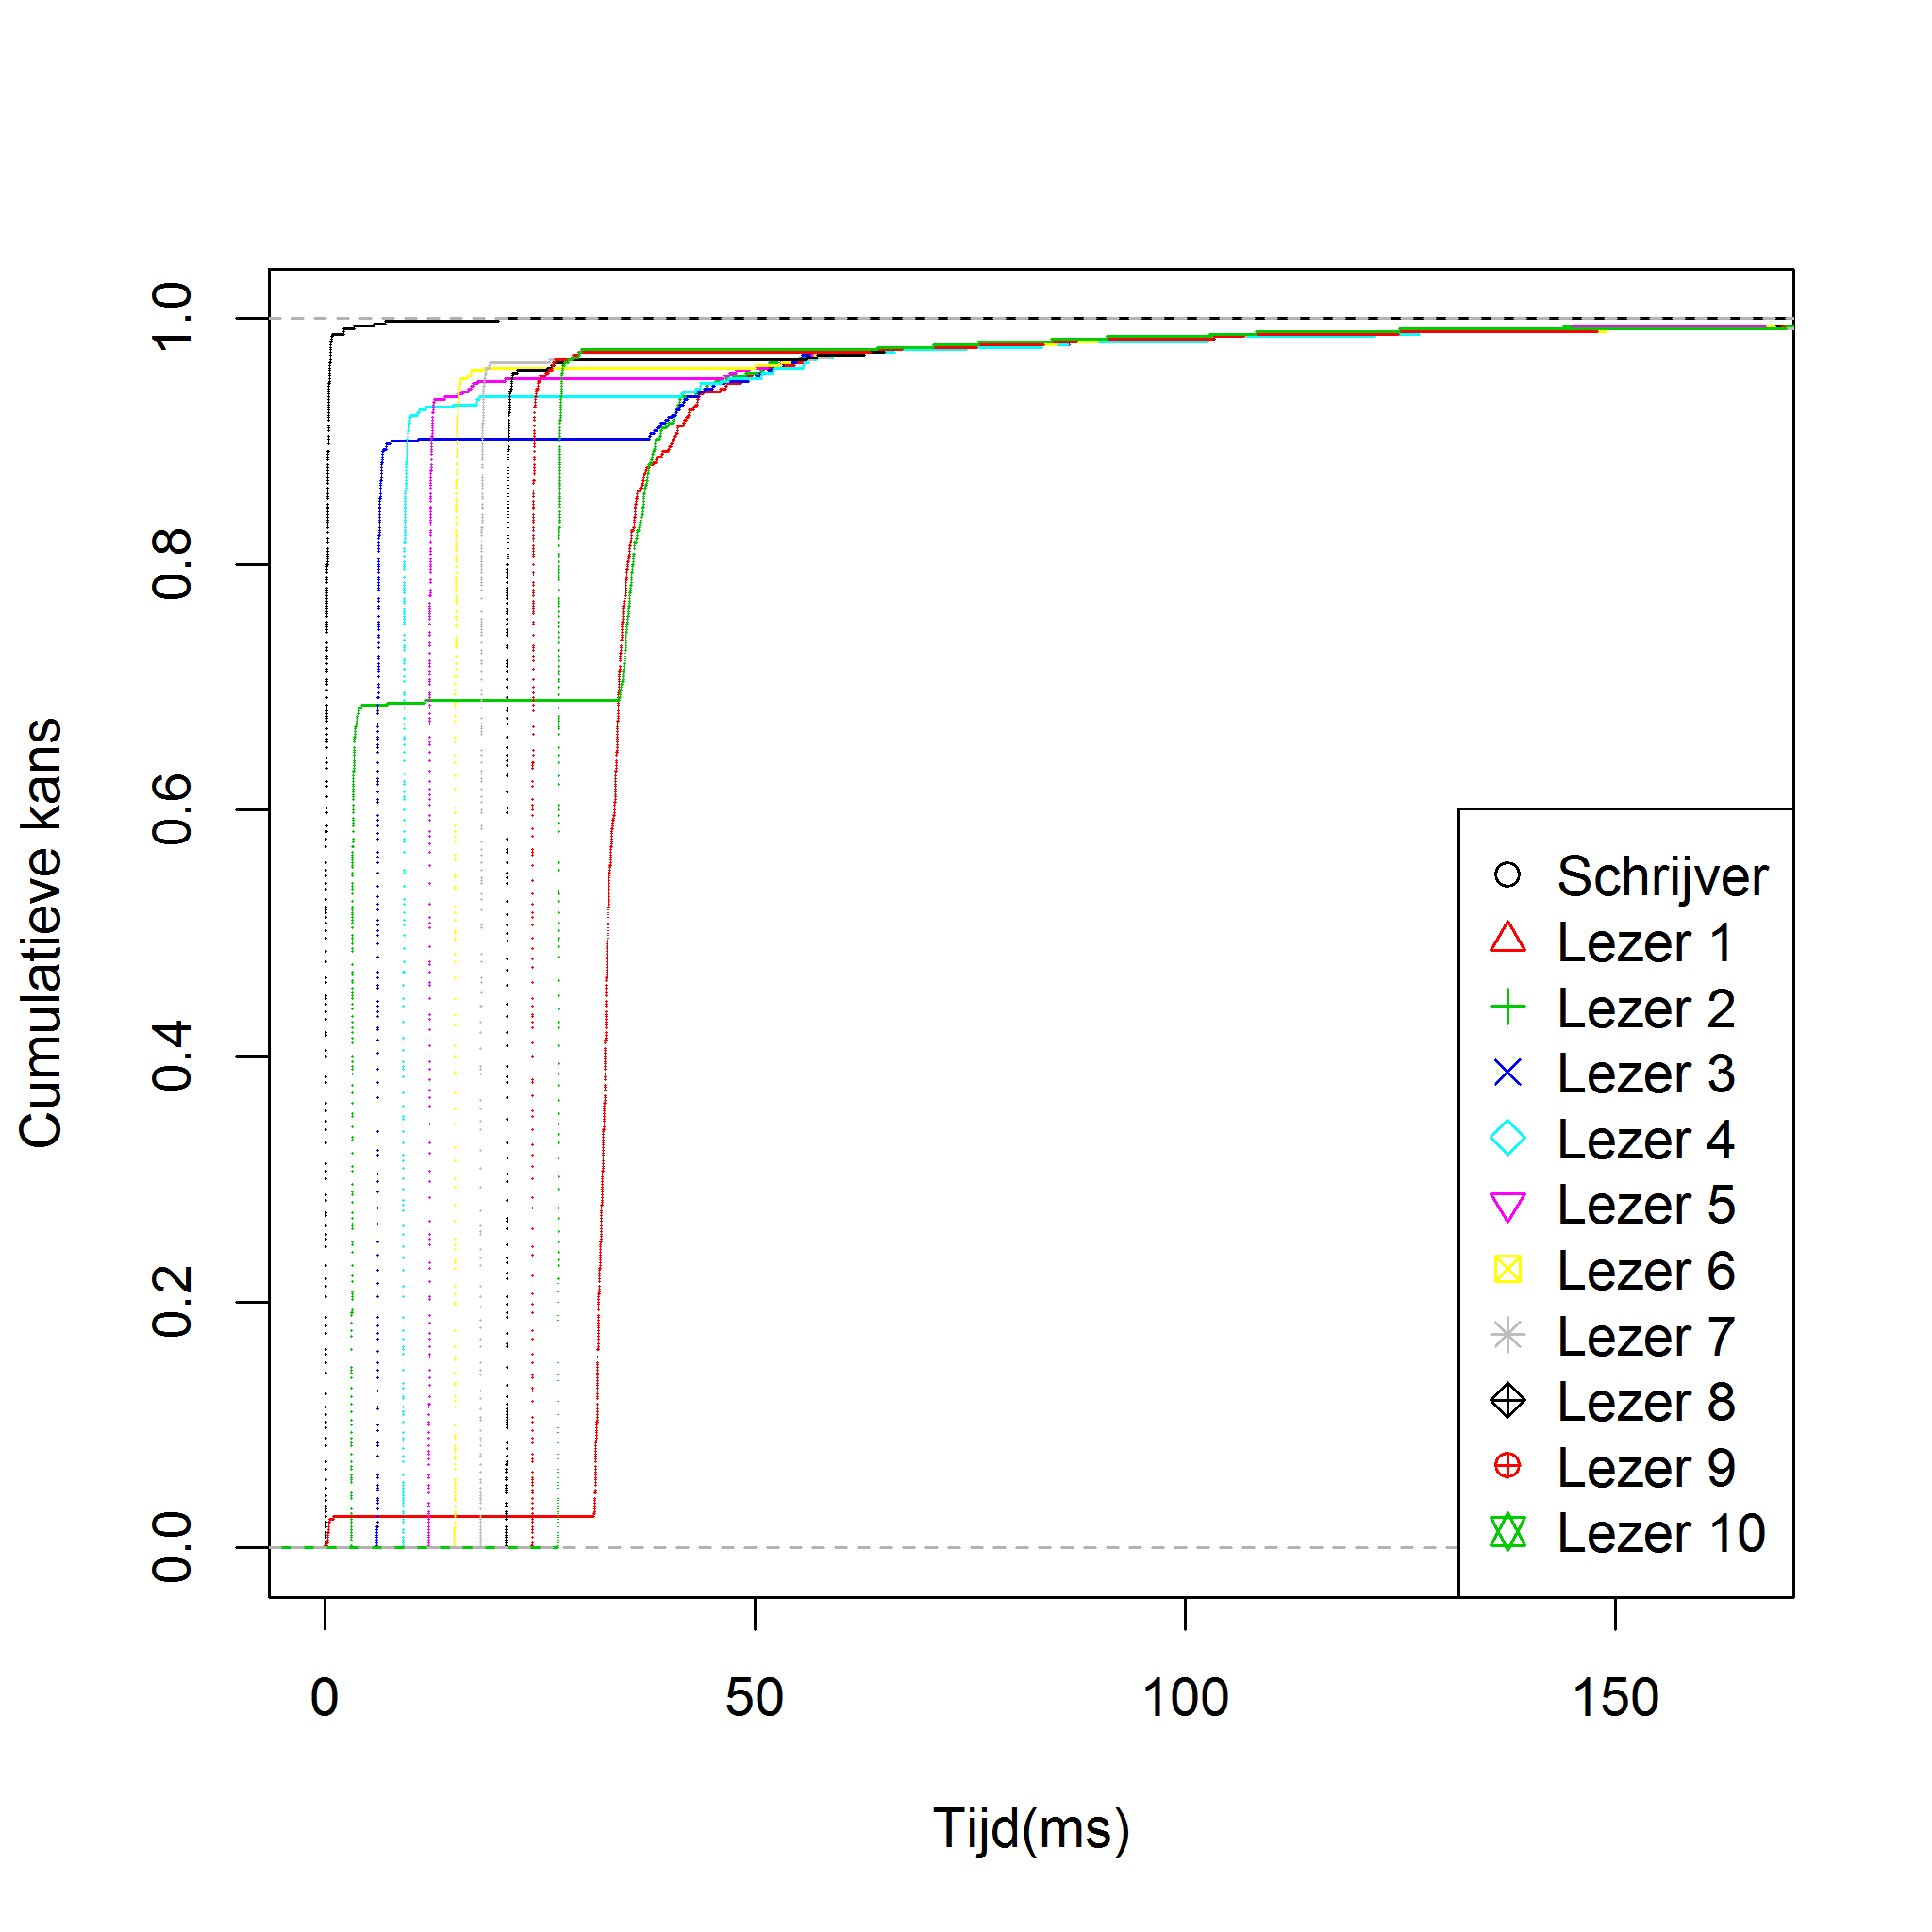
\includegraphics[width=.45\textwidth]{img/Observaties/HBase/ECDF-plot-Start-insertRawData-5}}
	\subfigure[De start- en stoptijdstippen voor lezer 2]{\label{fig:consistentie-hbase-R1} 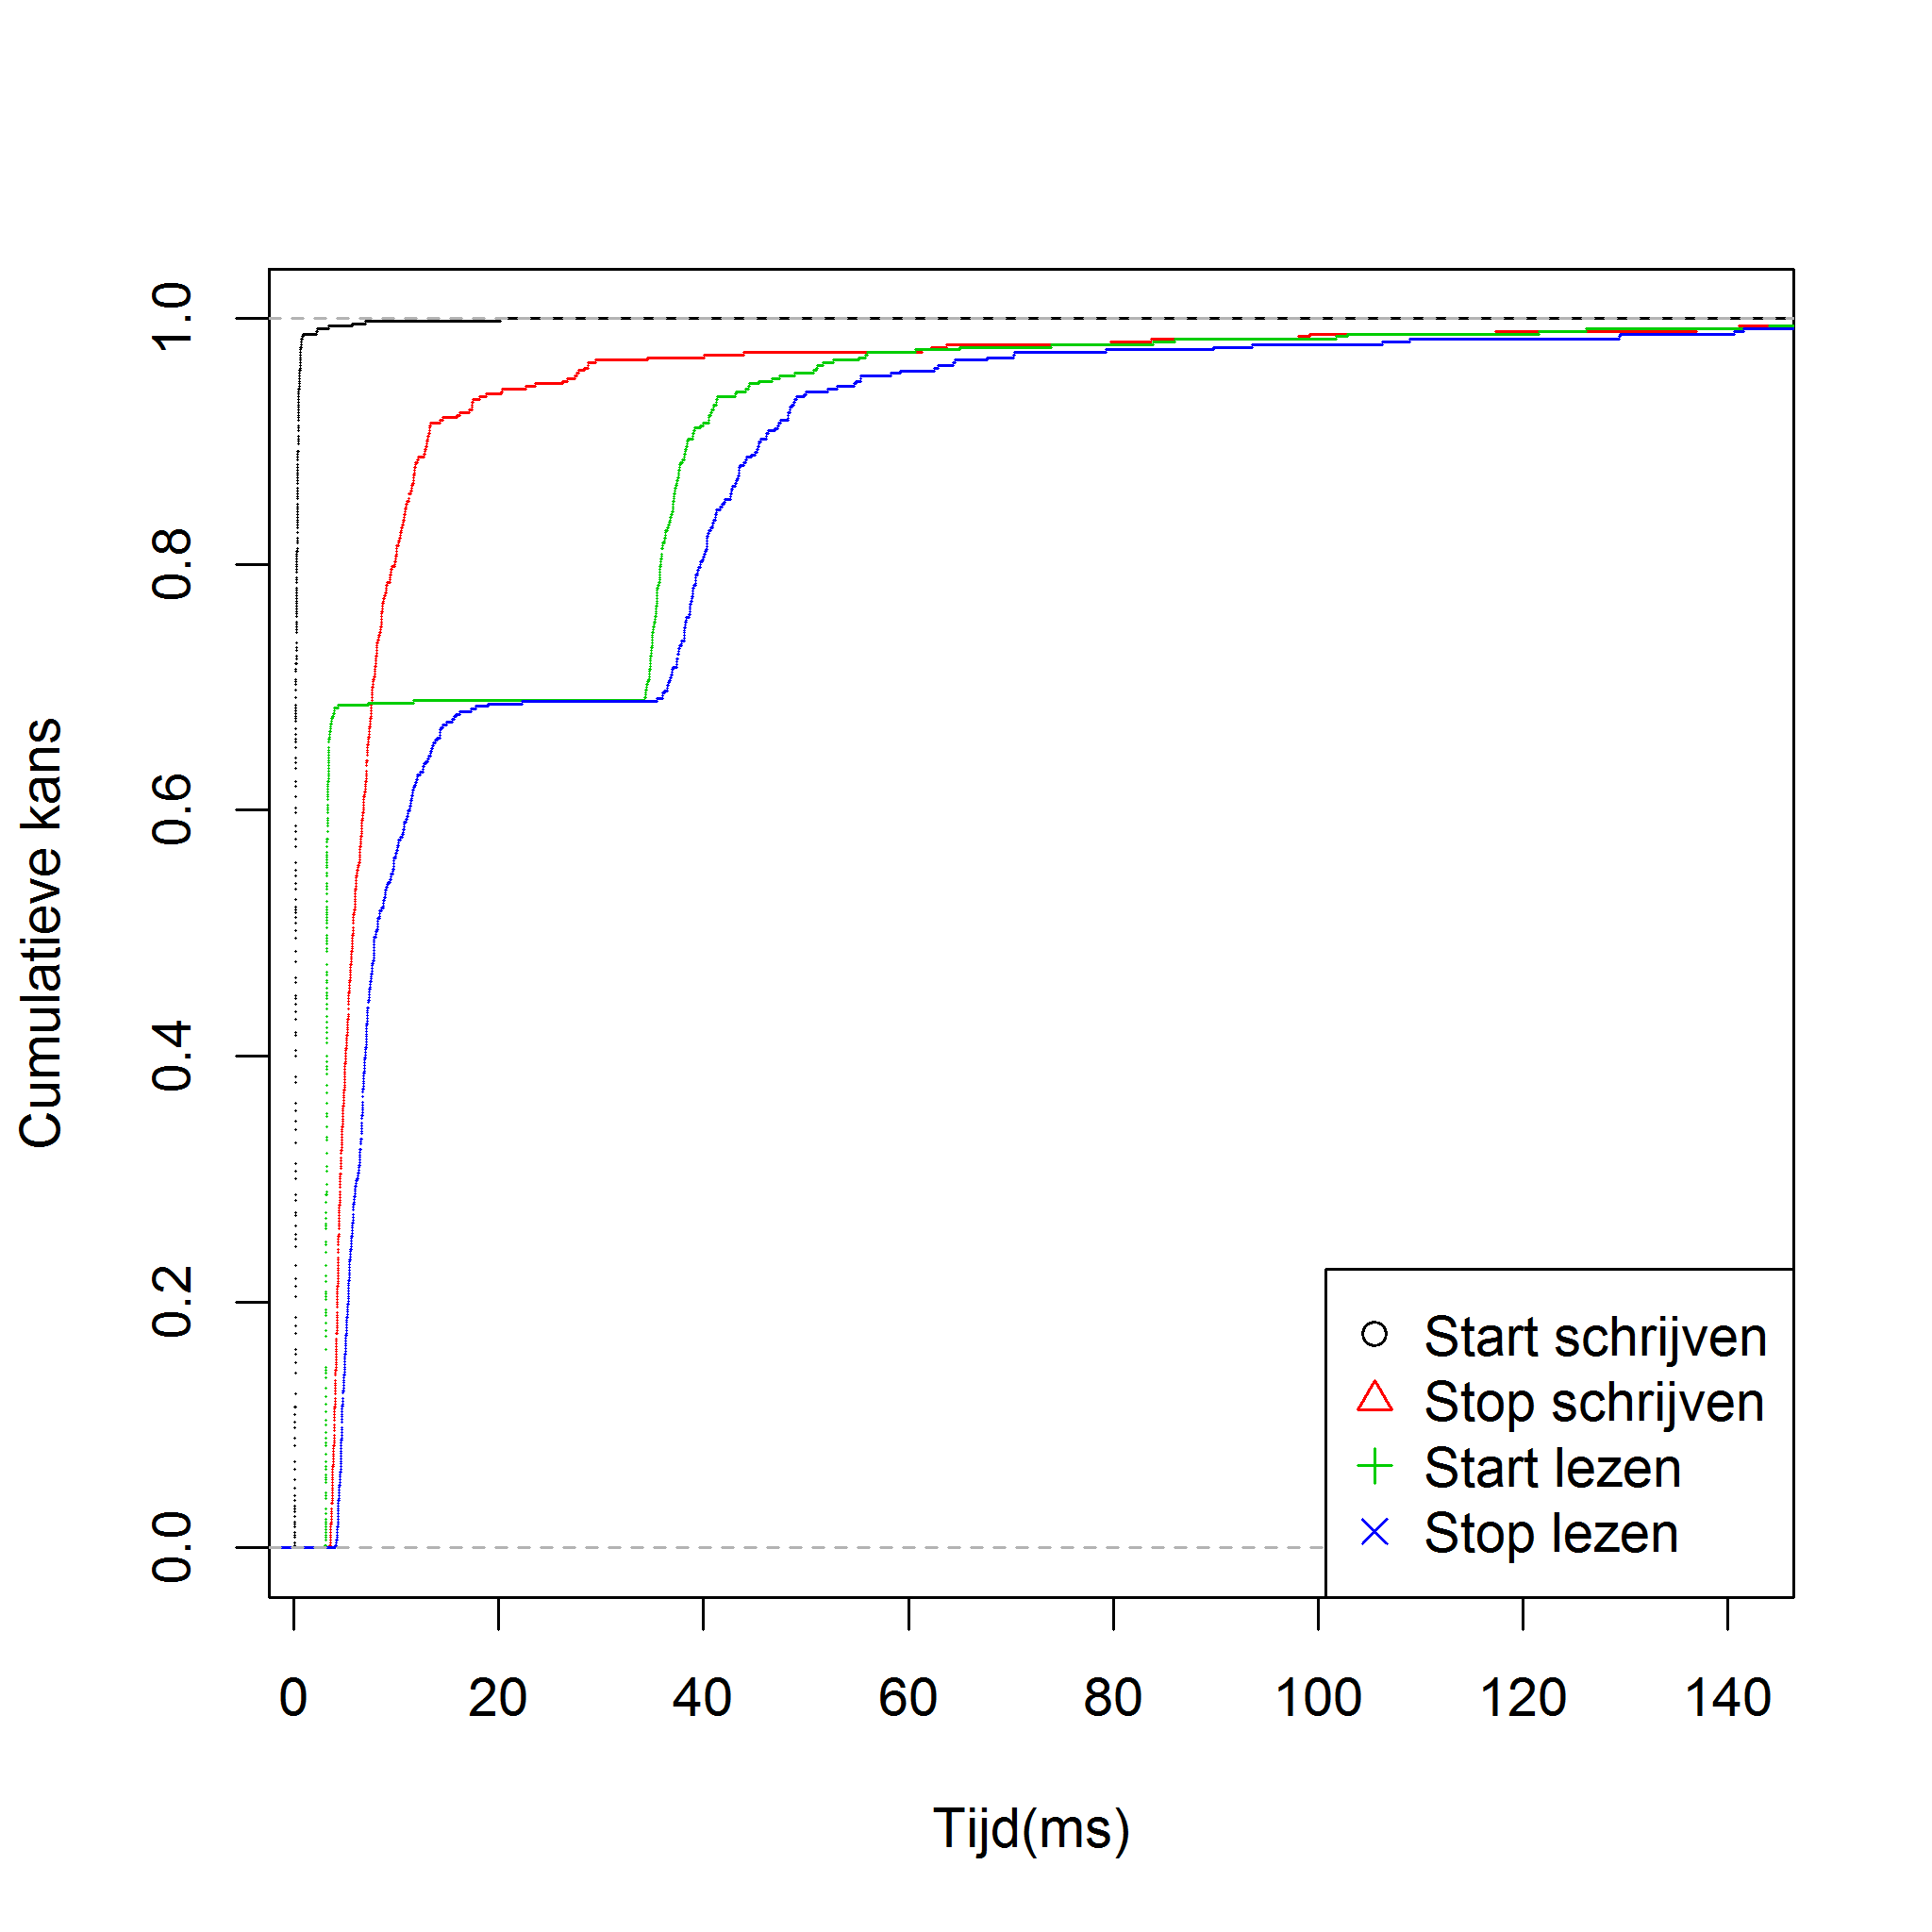
\includegraphics[width=0.45\textwidth]{img/Observaties/HBase/ECDF-plot-R-1-insertRawData-5}}

	\caption{Consistentie: Overzicht van HBase op de consistentie testen met een 99-percentiel.}
	\label{fig:consistentie-hbase}
\end{figure}

\begin{figure}[htb!] 
	\centering
	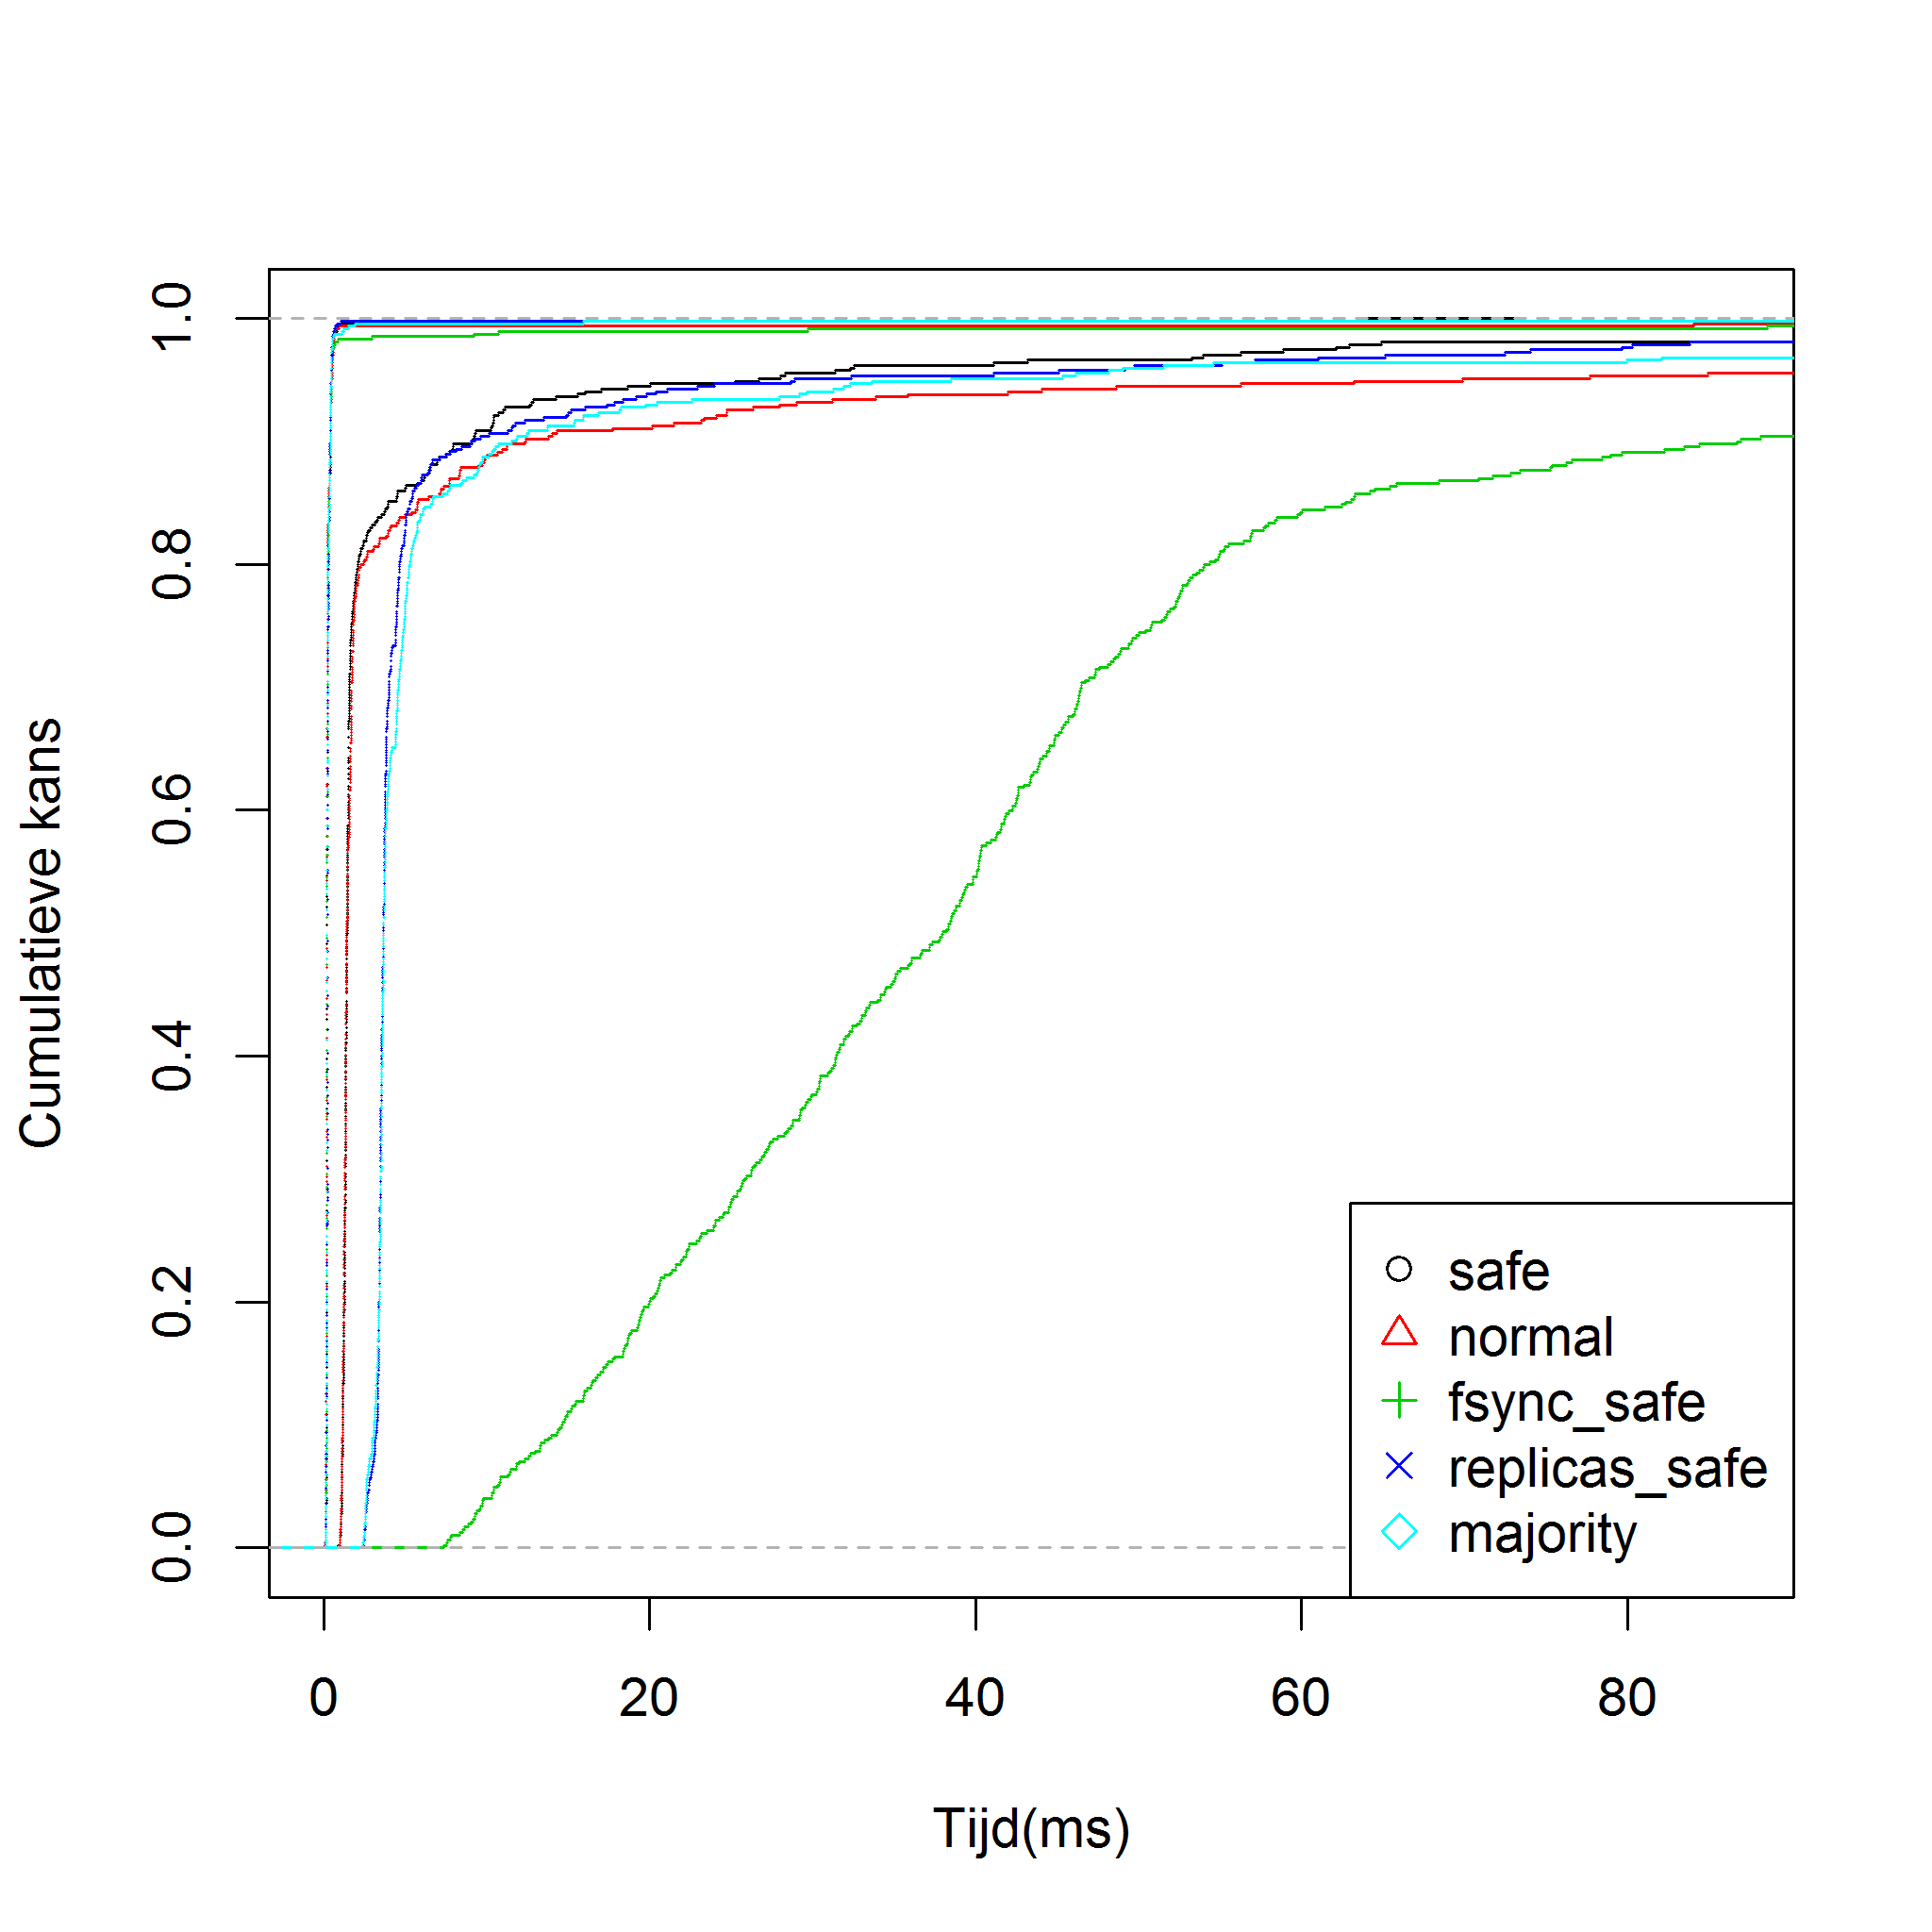
\includegraphics[width=.42\textwidth]{img/Observaties/MongoDB/ECDF-Compare-Write-insert-1}
	\caption{Consistentie: Overzicht van MongoDB's verschillende schrijfoperaties met een 90-percentiel met start en stoptijden in dezelfde kleur.  }
	\label{fig:consistentie-mongodb-all-mongodb-write}
\end{figure}

\begin{figure}[ht!] 
	\centering
	\subfigure[Normal Update]{\label{fig:consistentie-all-mongodb-normal} 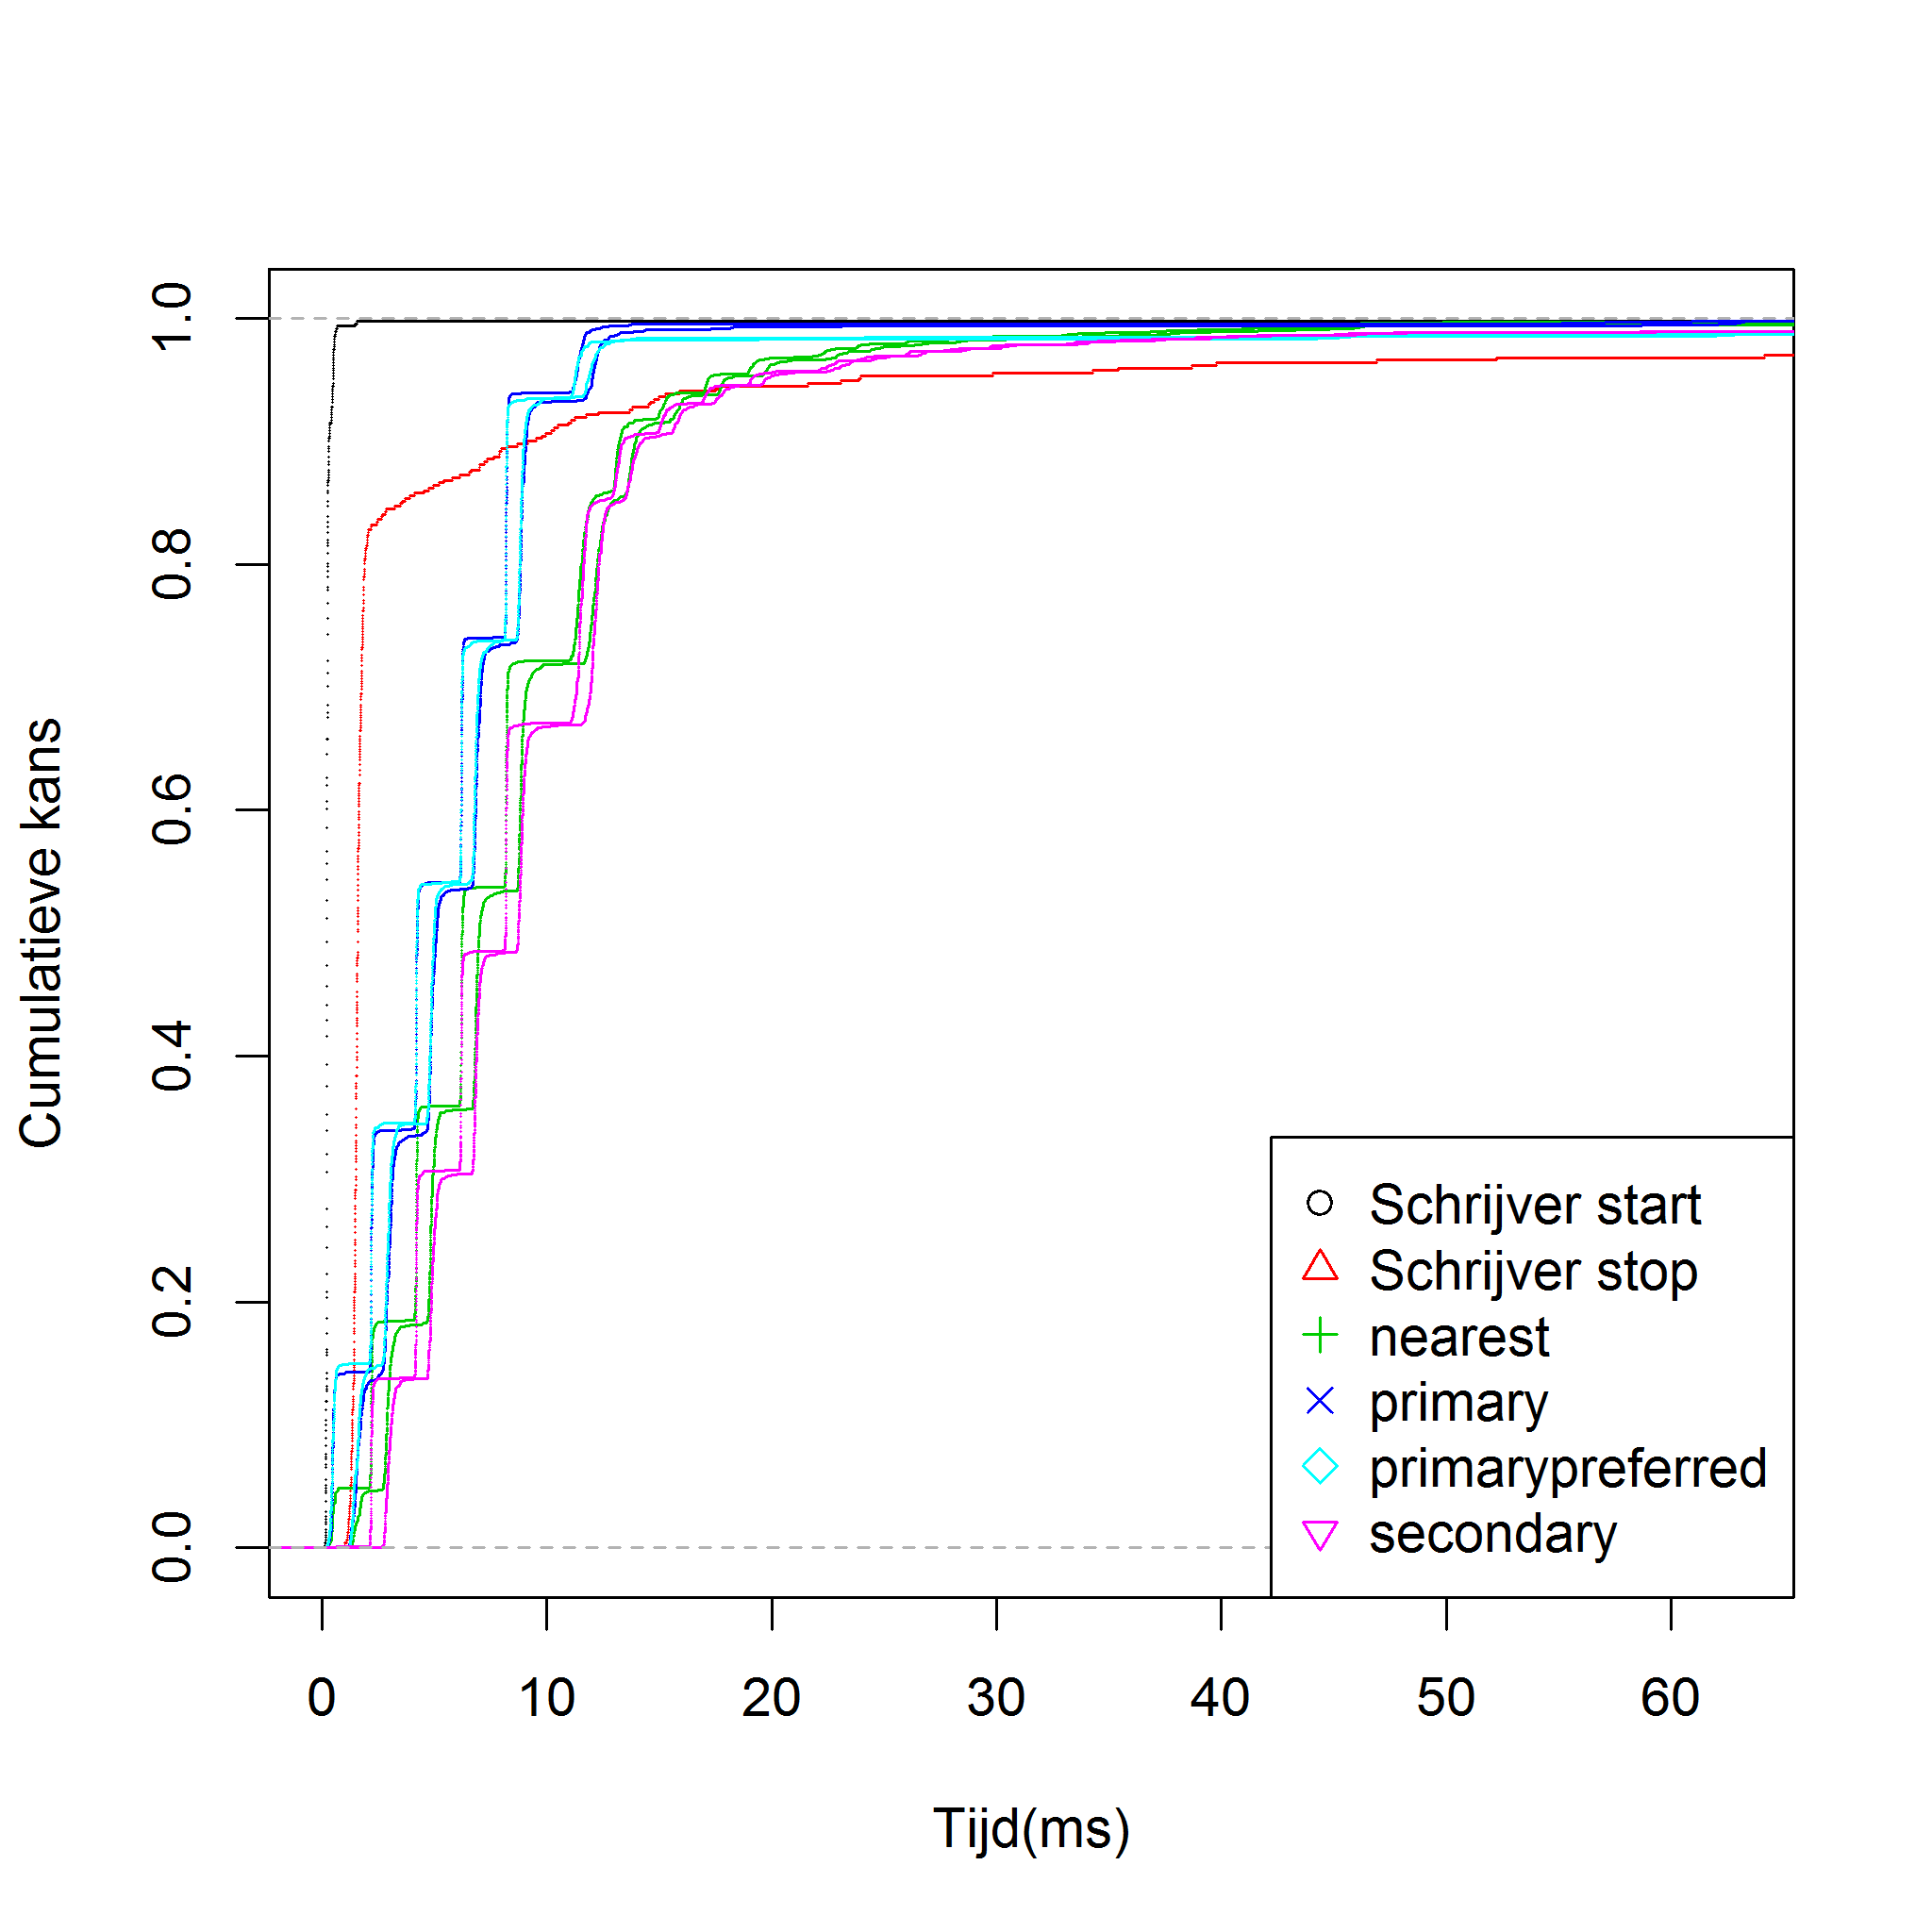
\includegraphics[width=.40\textwidth]{img/Observaties/MongoDB/ECDF-Reads-update-normal-all-2}}
	\subfigure[Safe Update]{\label{fig:consistentie-all-mongodb-safe} 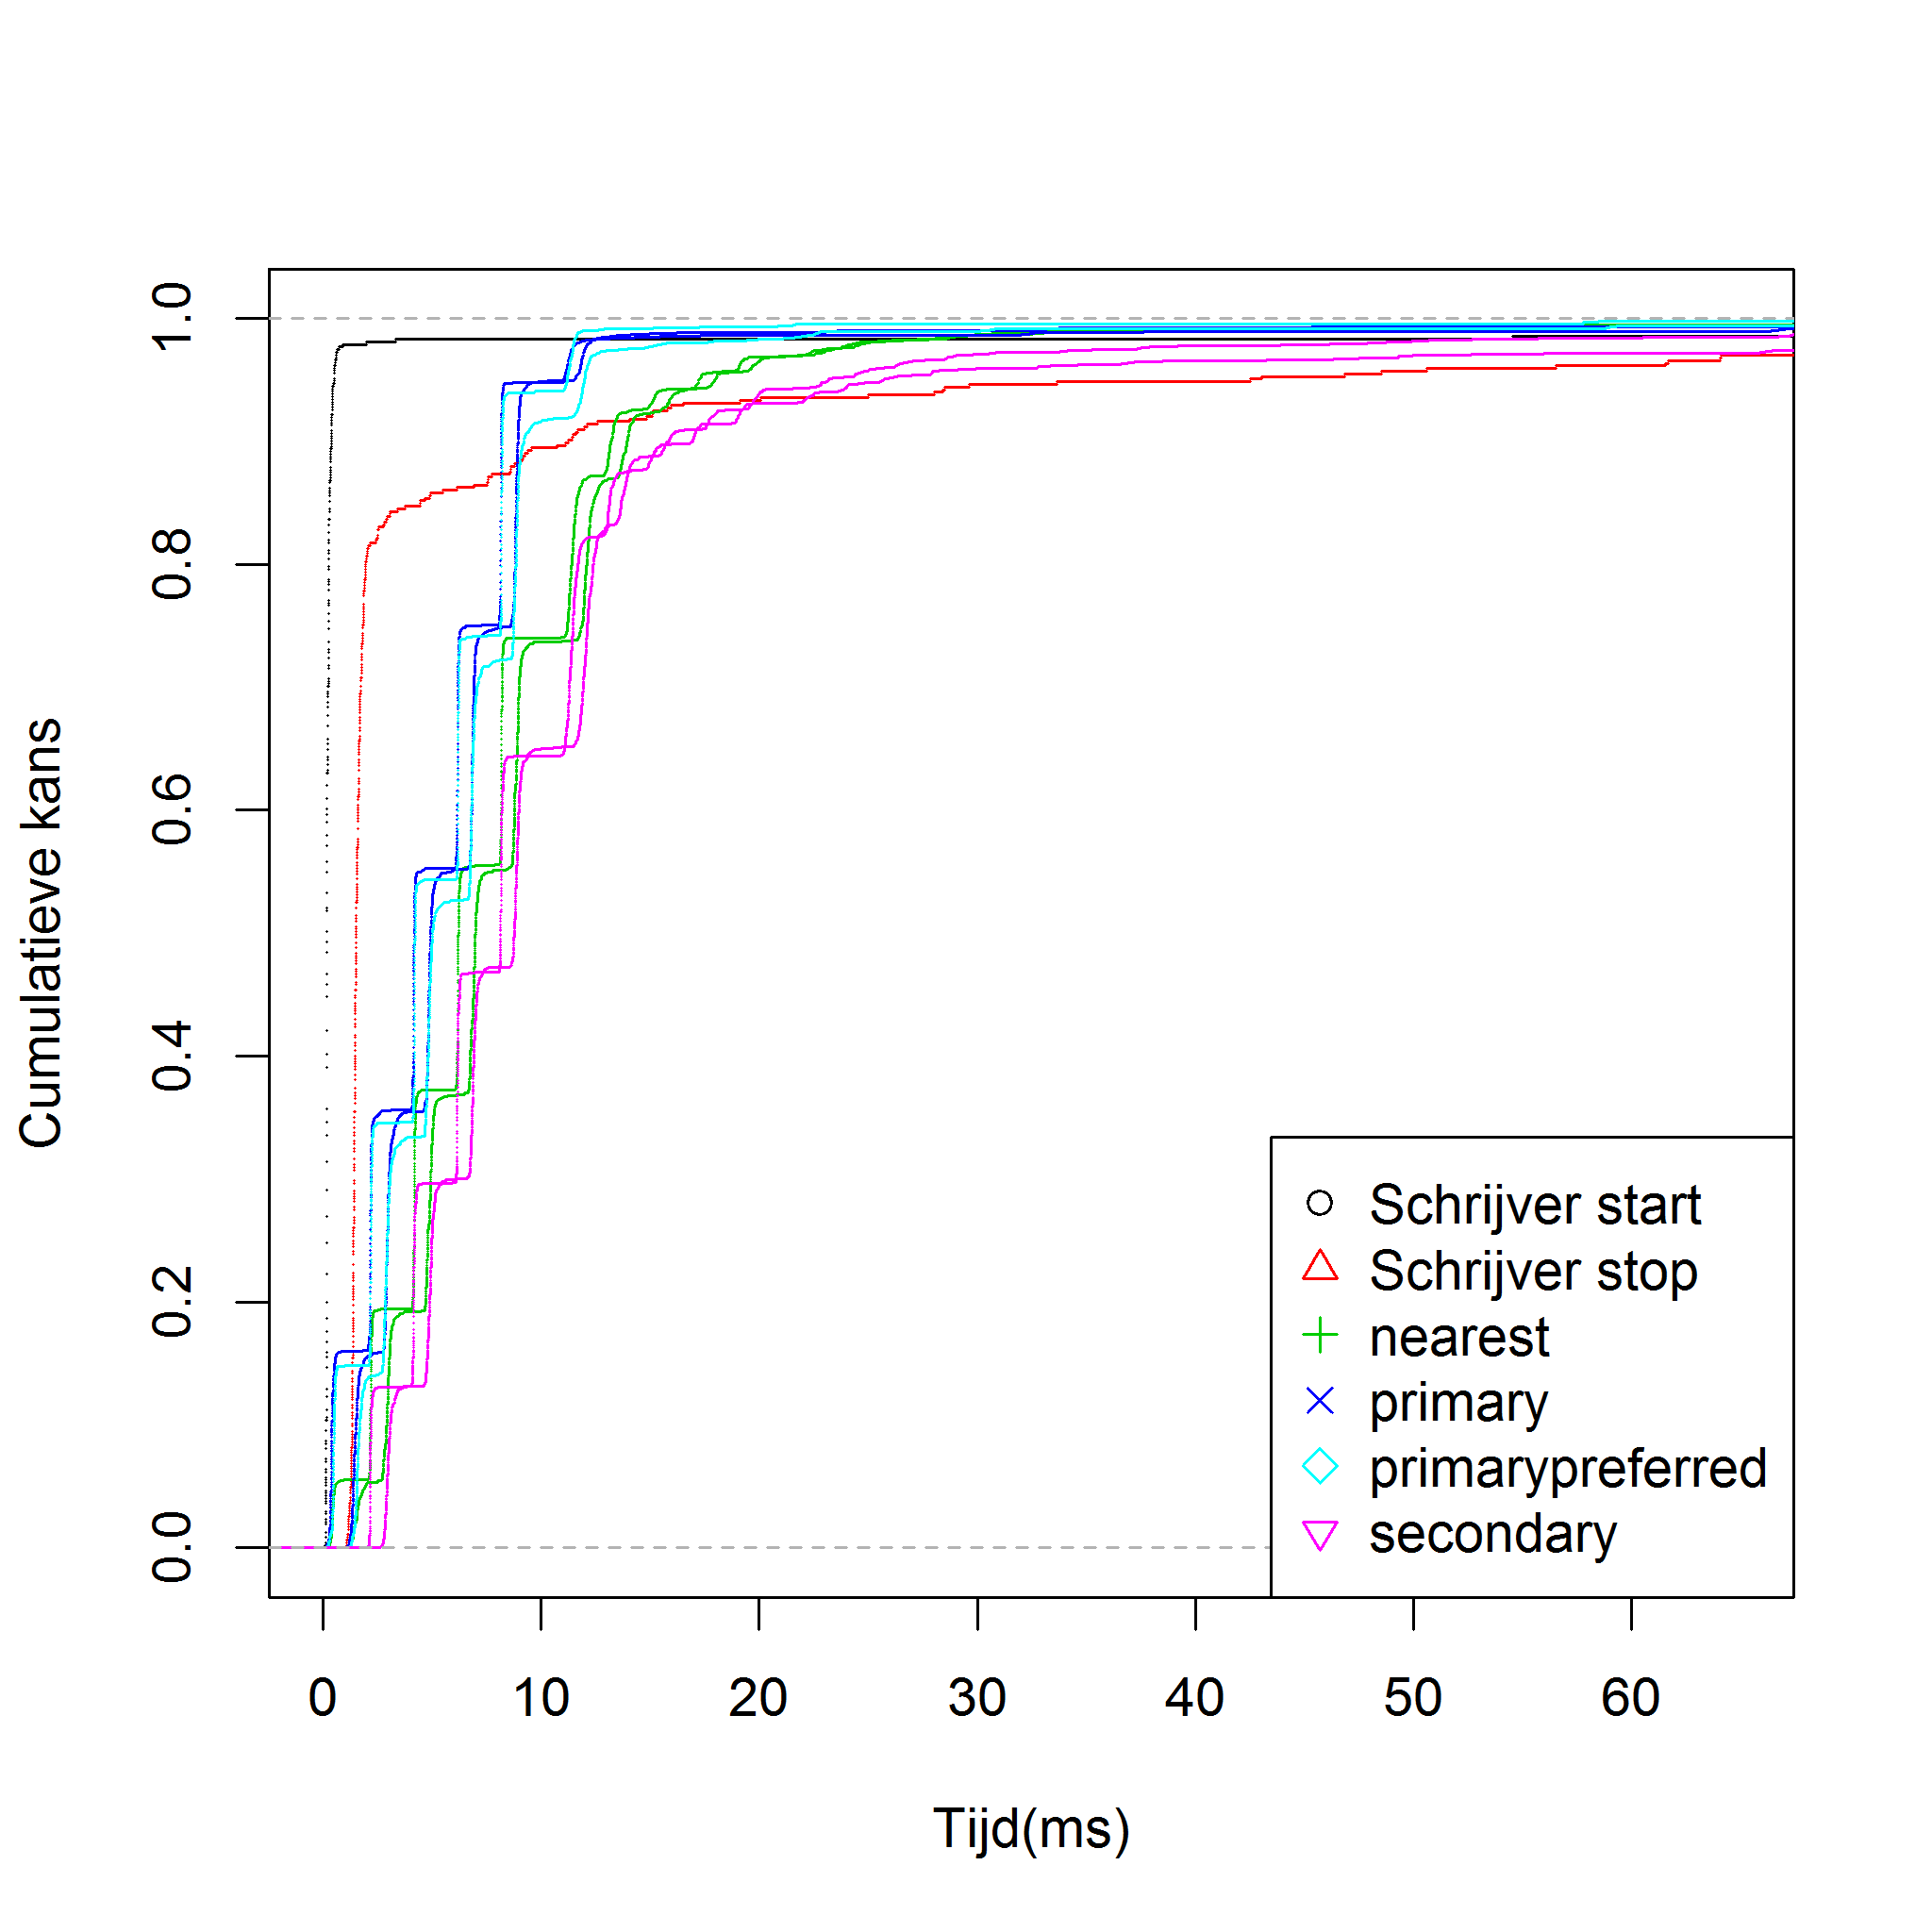
\includegraphics[width=.40\textwidth]{img/Observaties/MongoDB/ECDF-Reads-update-safe-all-2}}
	\subfigure[Fsync Safe Update]{\label{fig:consistentie-all-mongodb-fsync} 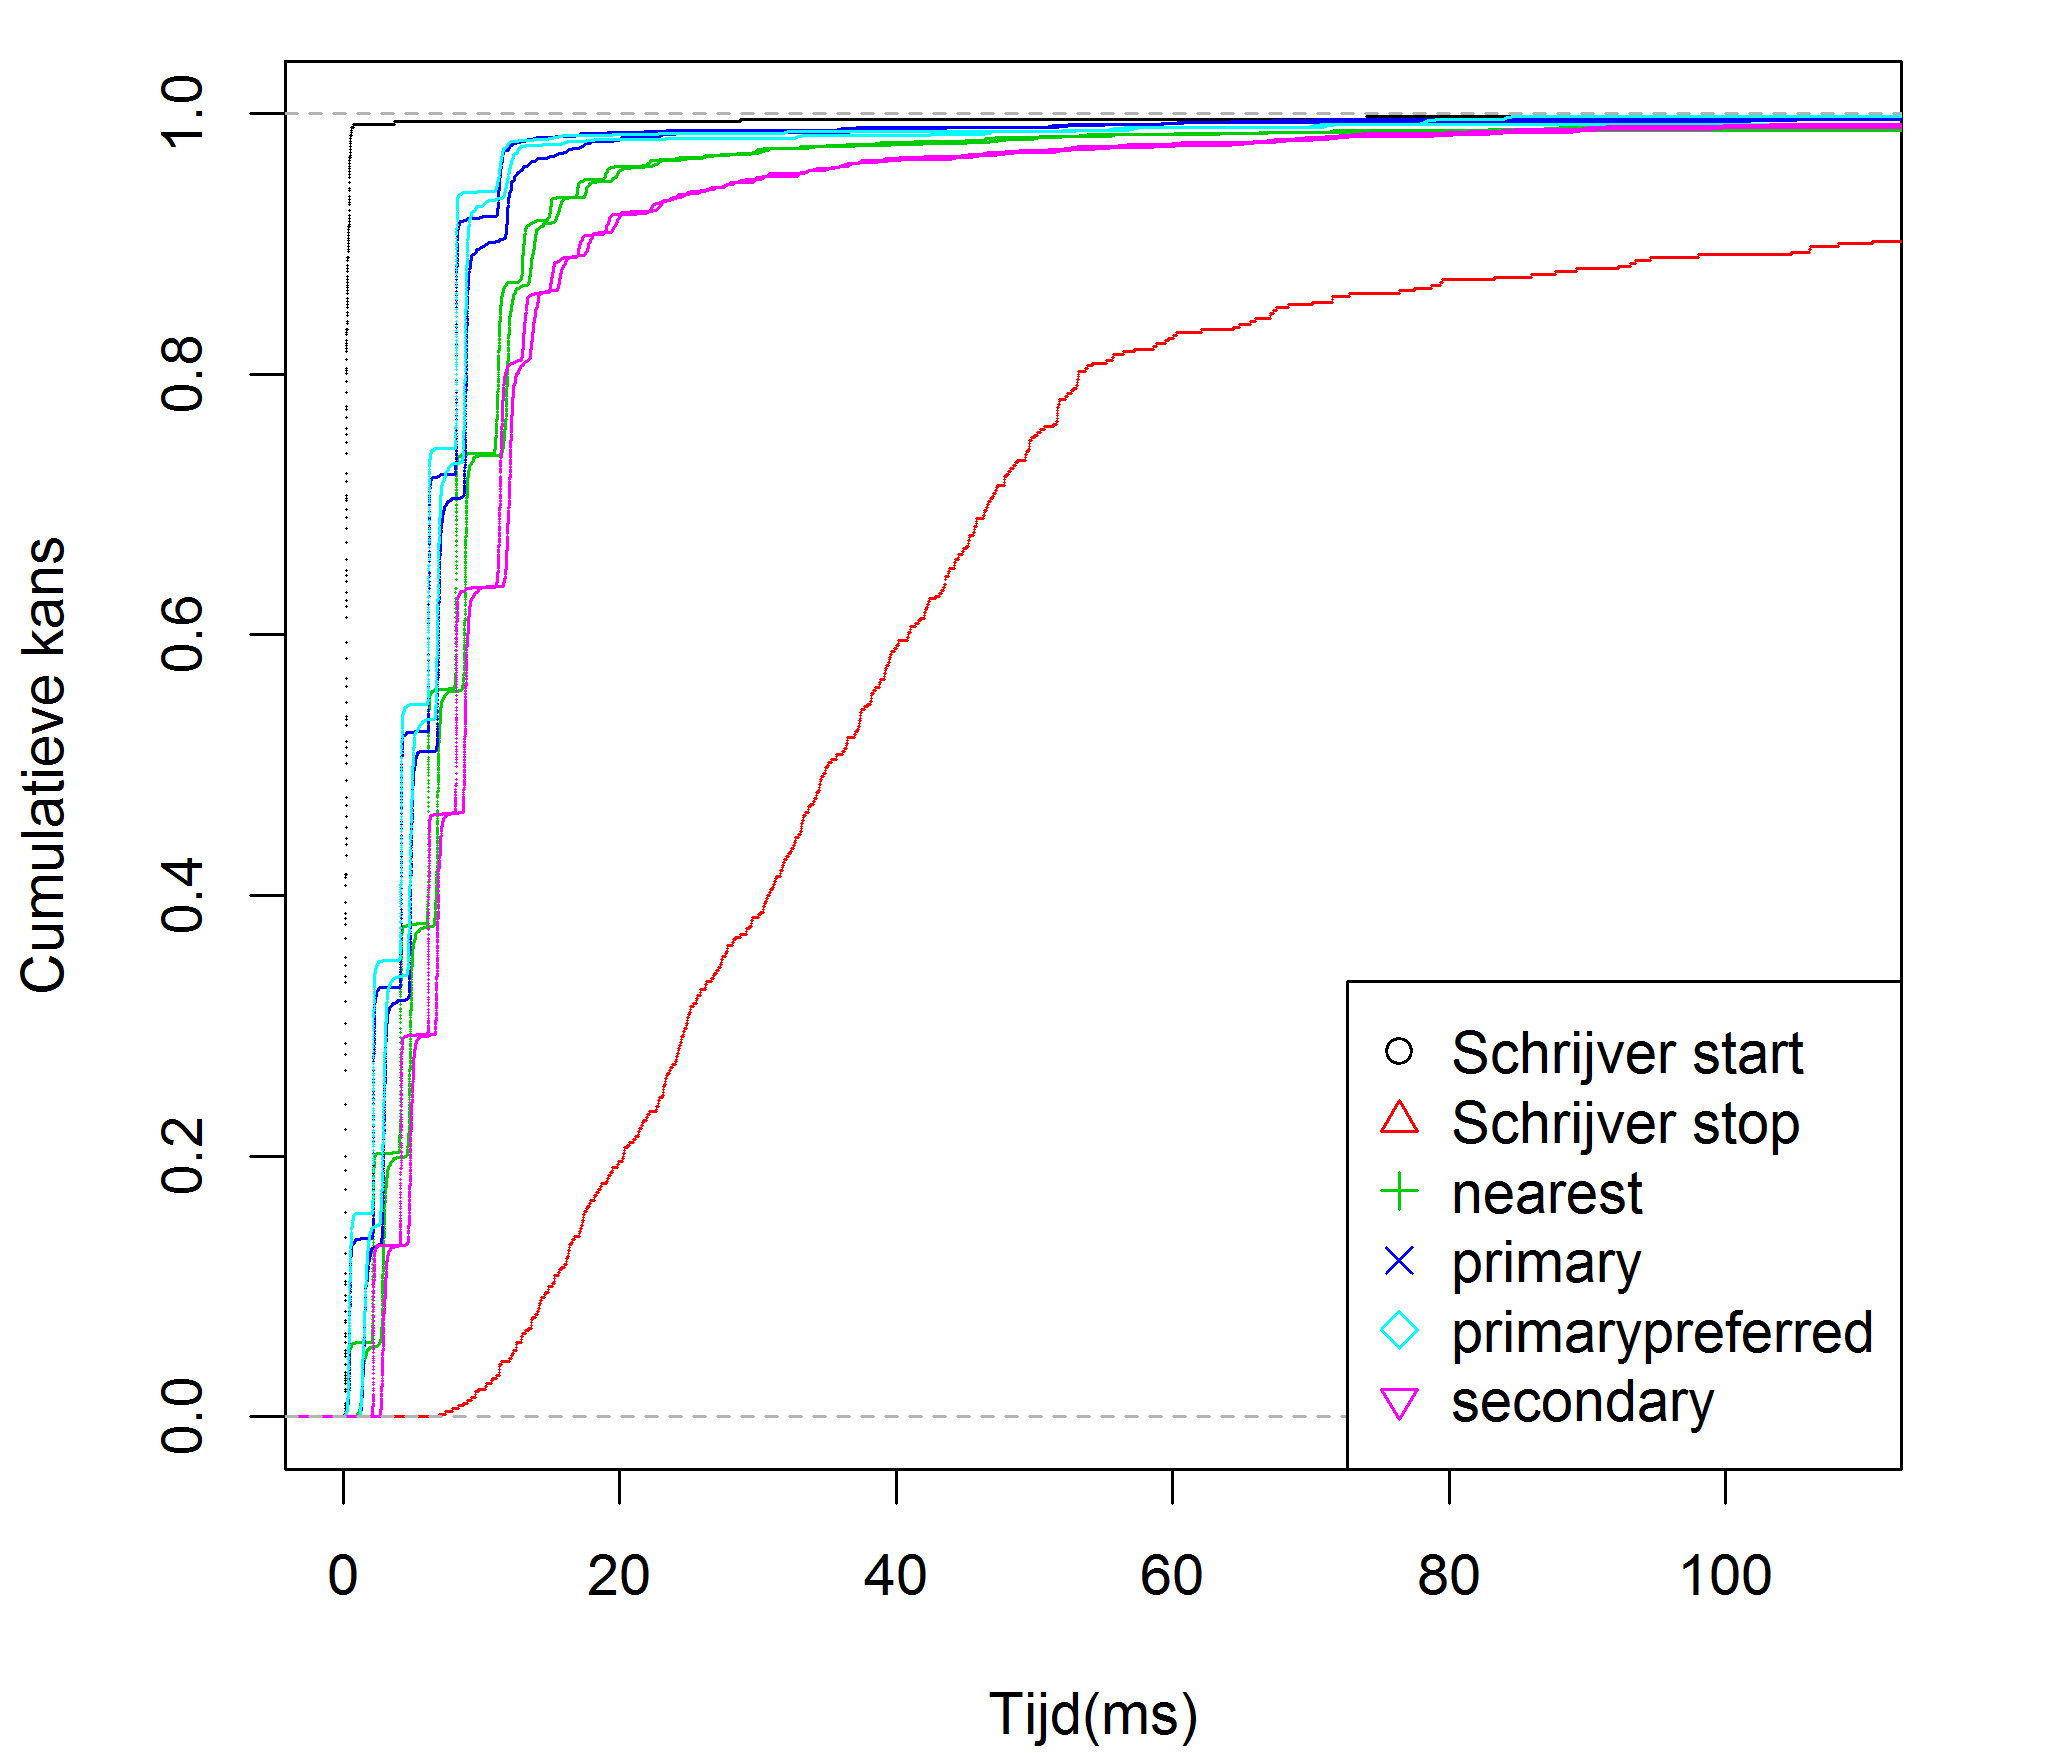
\includegraphics[width=.42\textwidth]{img/Observaties/MongoDB/ECDF-Reads-update-fsync_safe-all-2}}
	\subfigure[Replica Safe Update]{\label{fig:consistentie-all-mongodb-replicasafe} 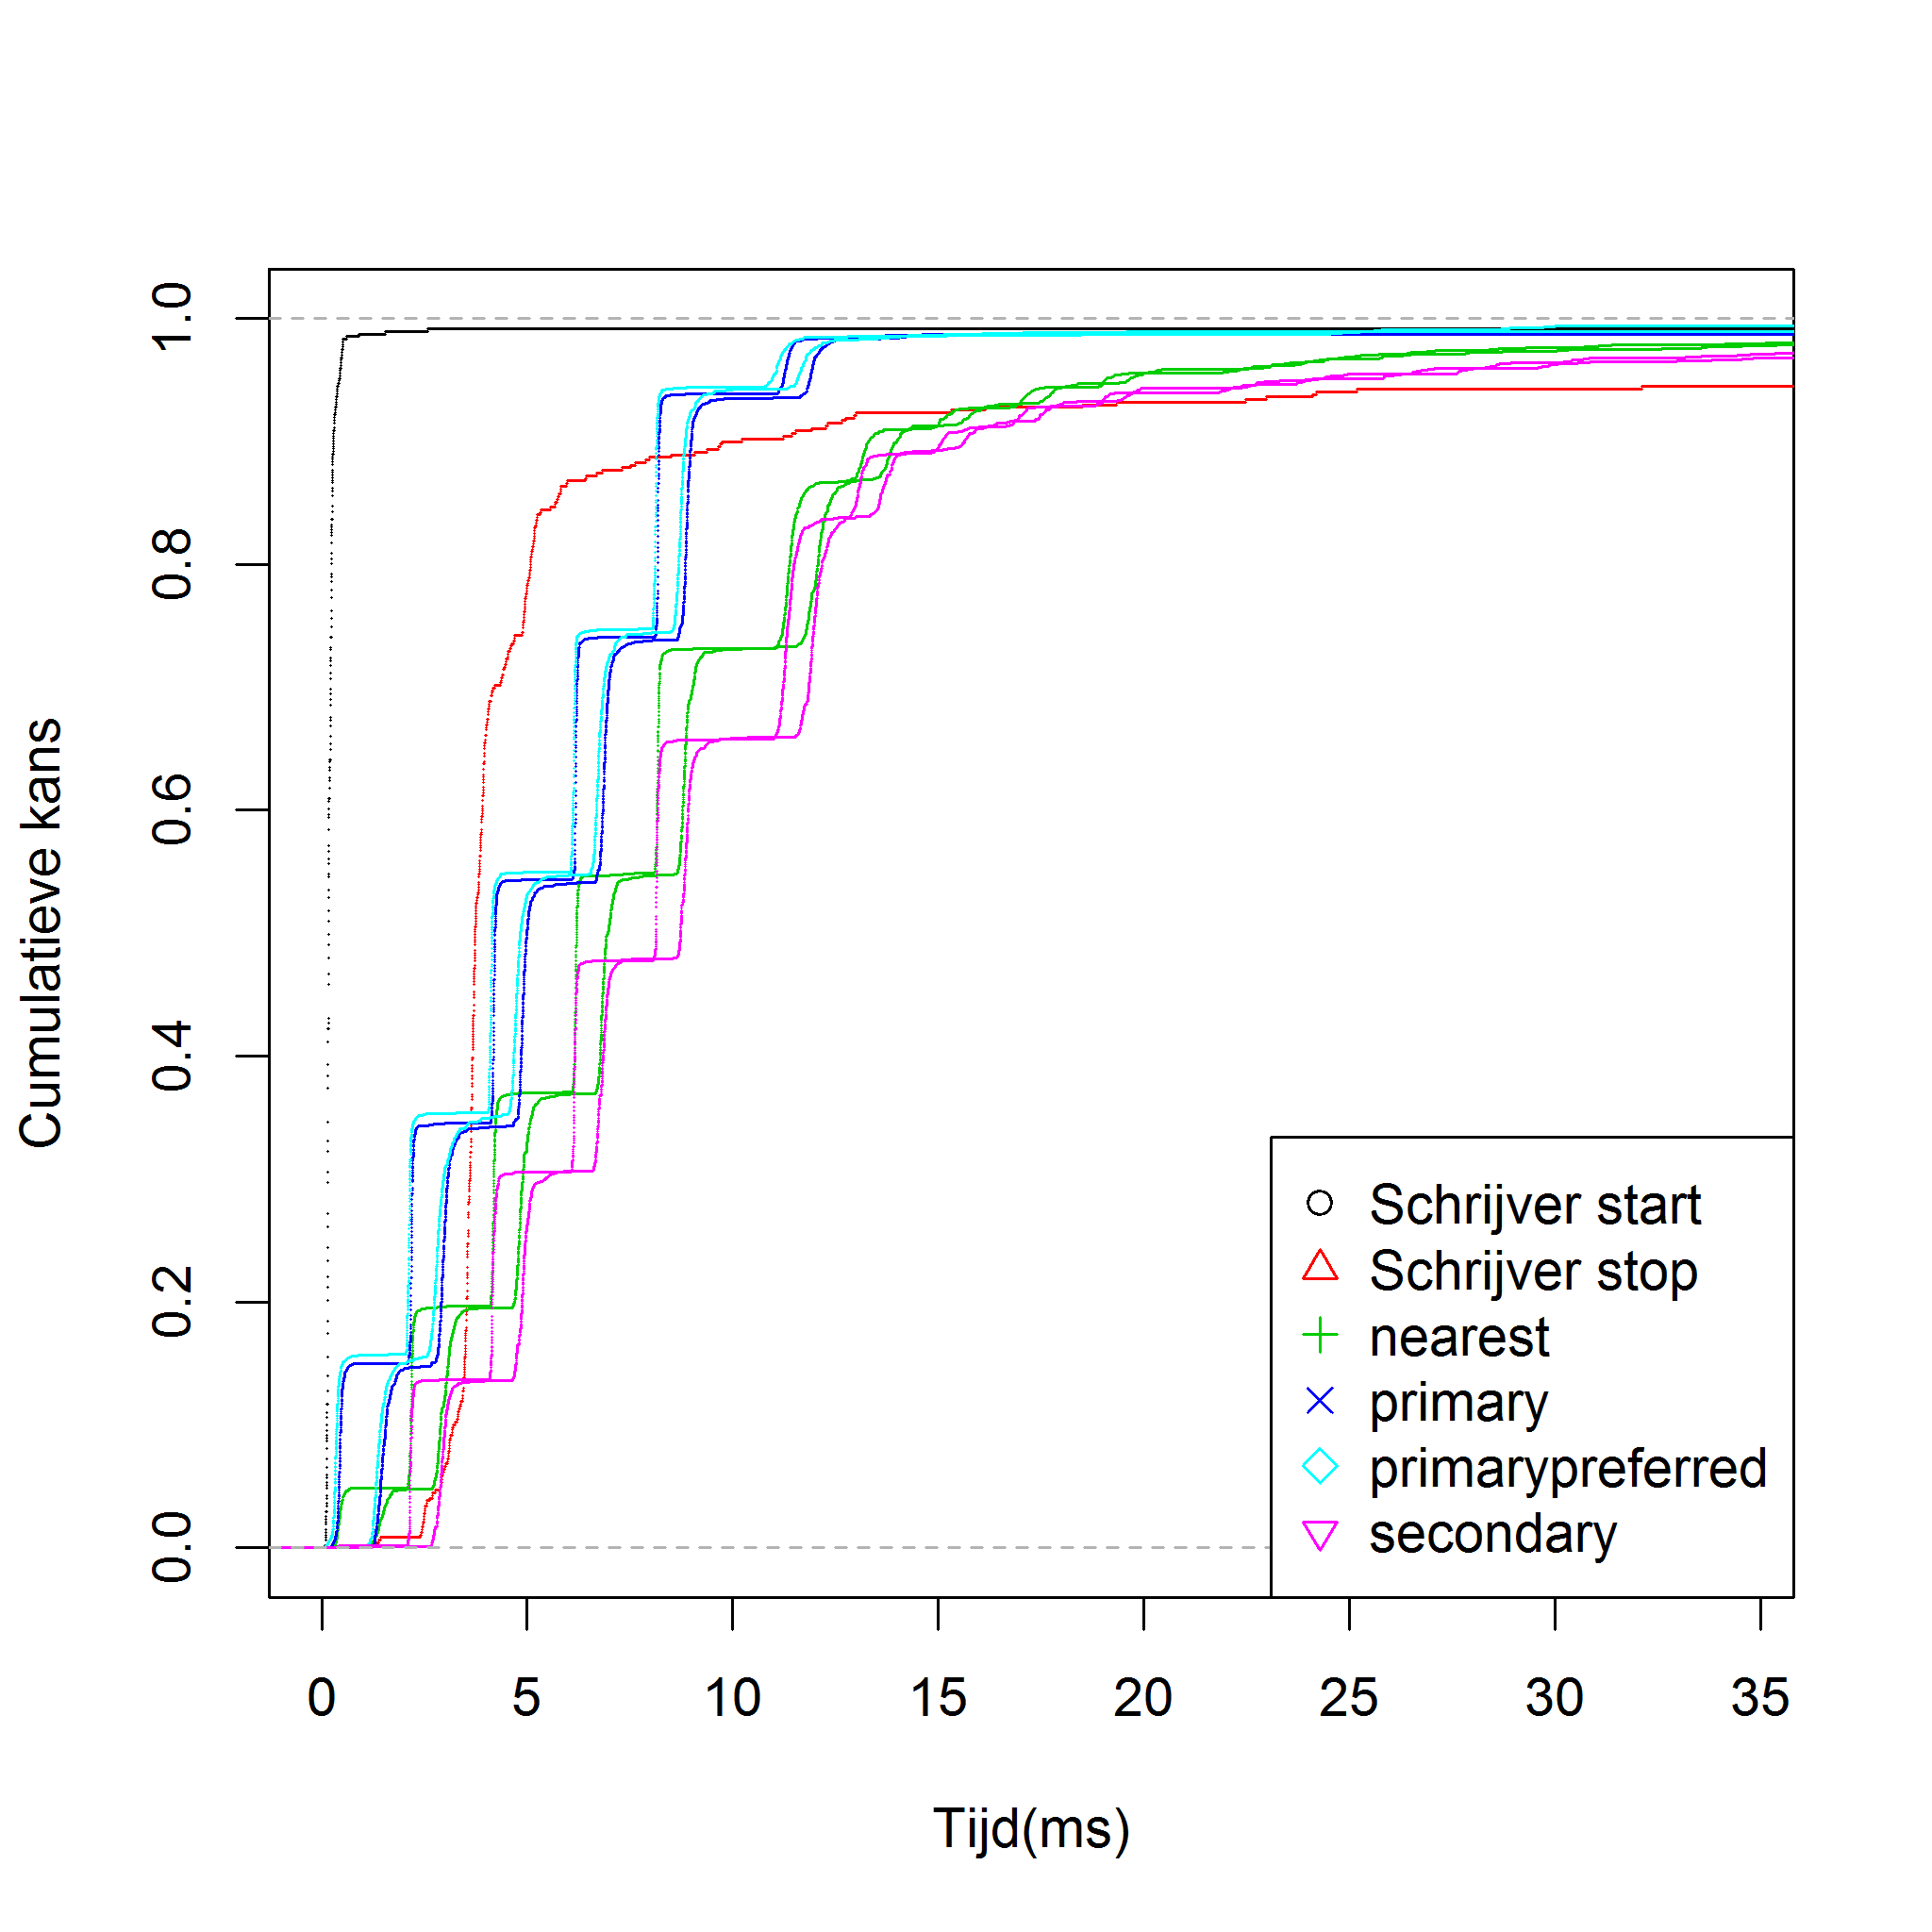
\includegraphics[width=.40\textwidth]{img/Observaties/MongoDB/ECDF-Reads-update-replicas_safe-all-2}}
	\subfigure[Majority Update]{\label{fig:consistentie-mongodb-all-majority} 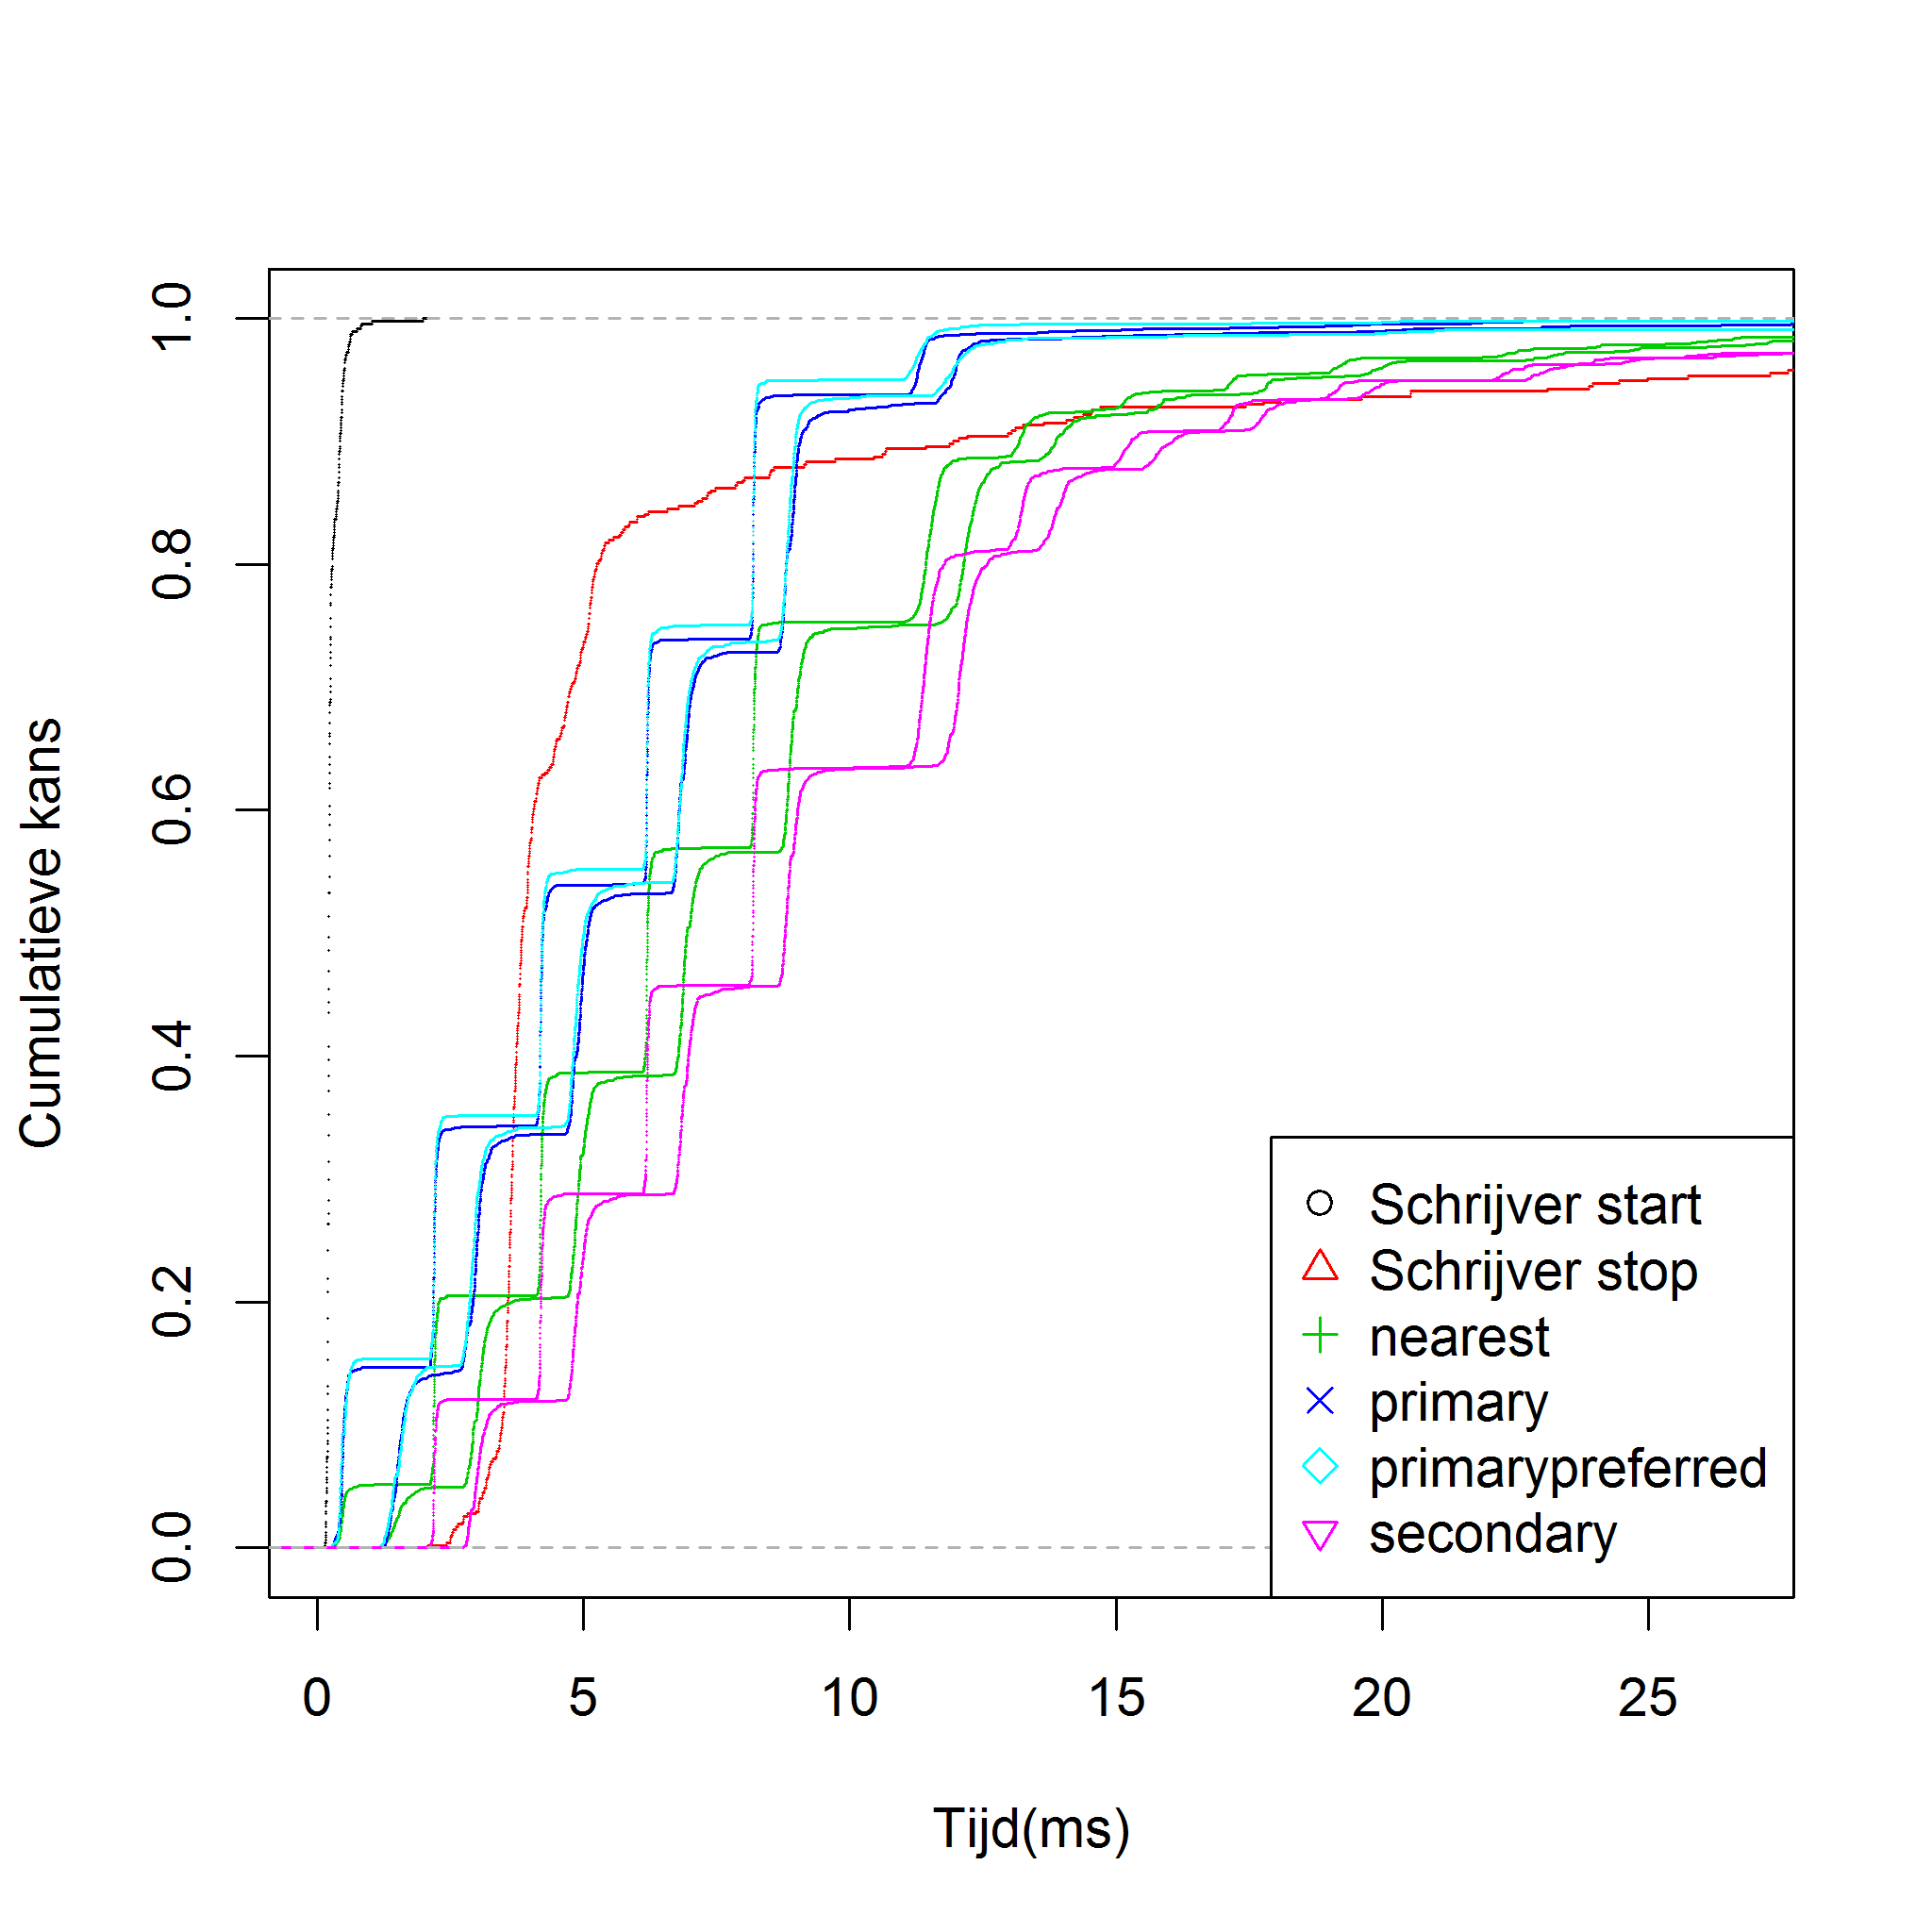
\includegraphics[width=.40\textwidth]{img/Observaties/MongoDB/ECDF-Reads-update-majority-all-2}}
	\subfigure[Majority Insert]{\label{fig:consistentie-mongodb-all-majority-insert} 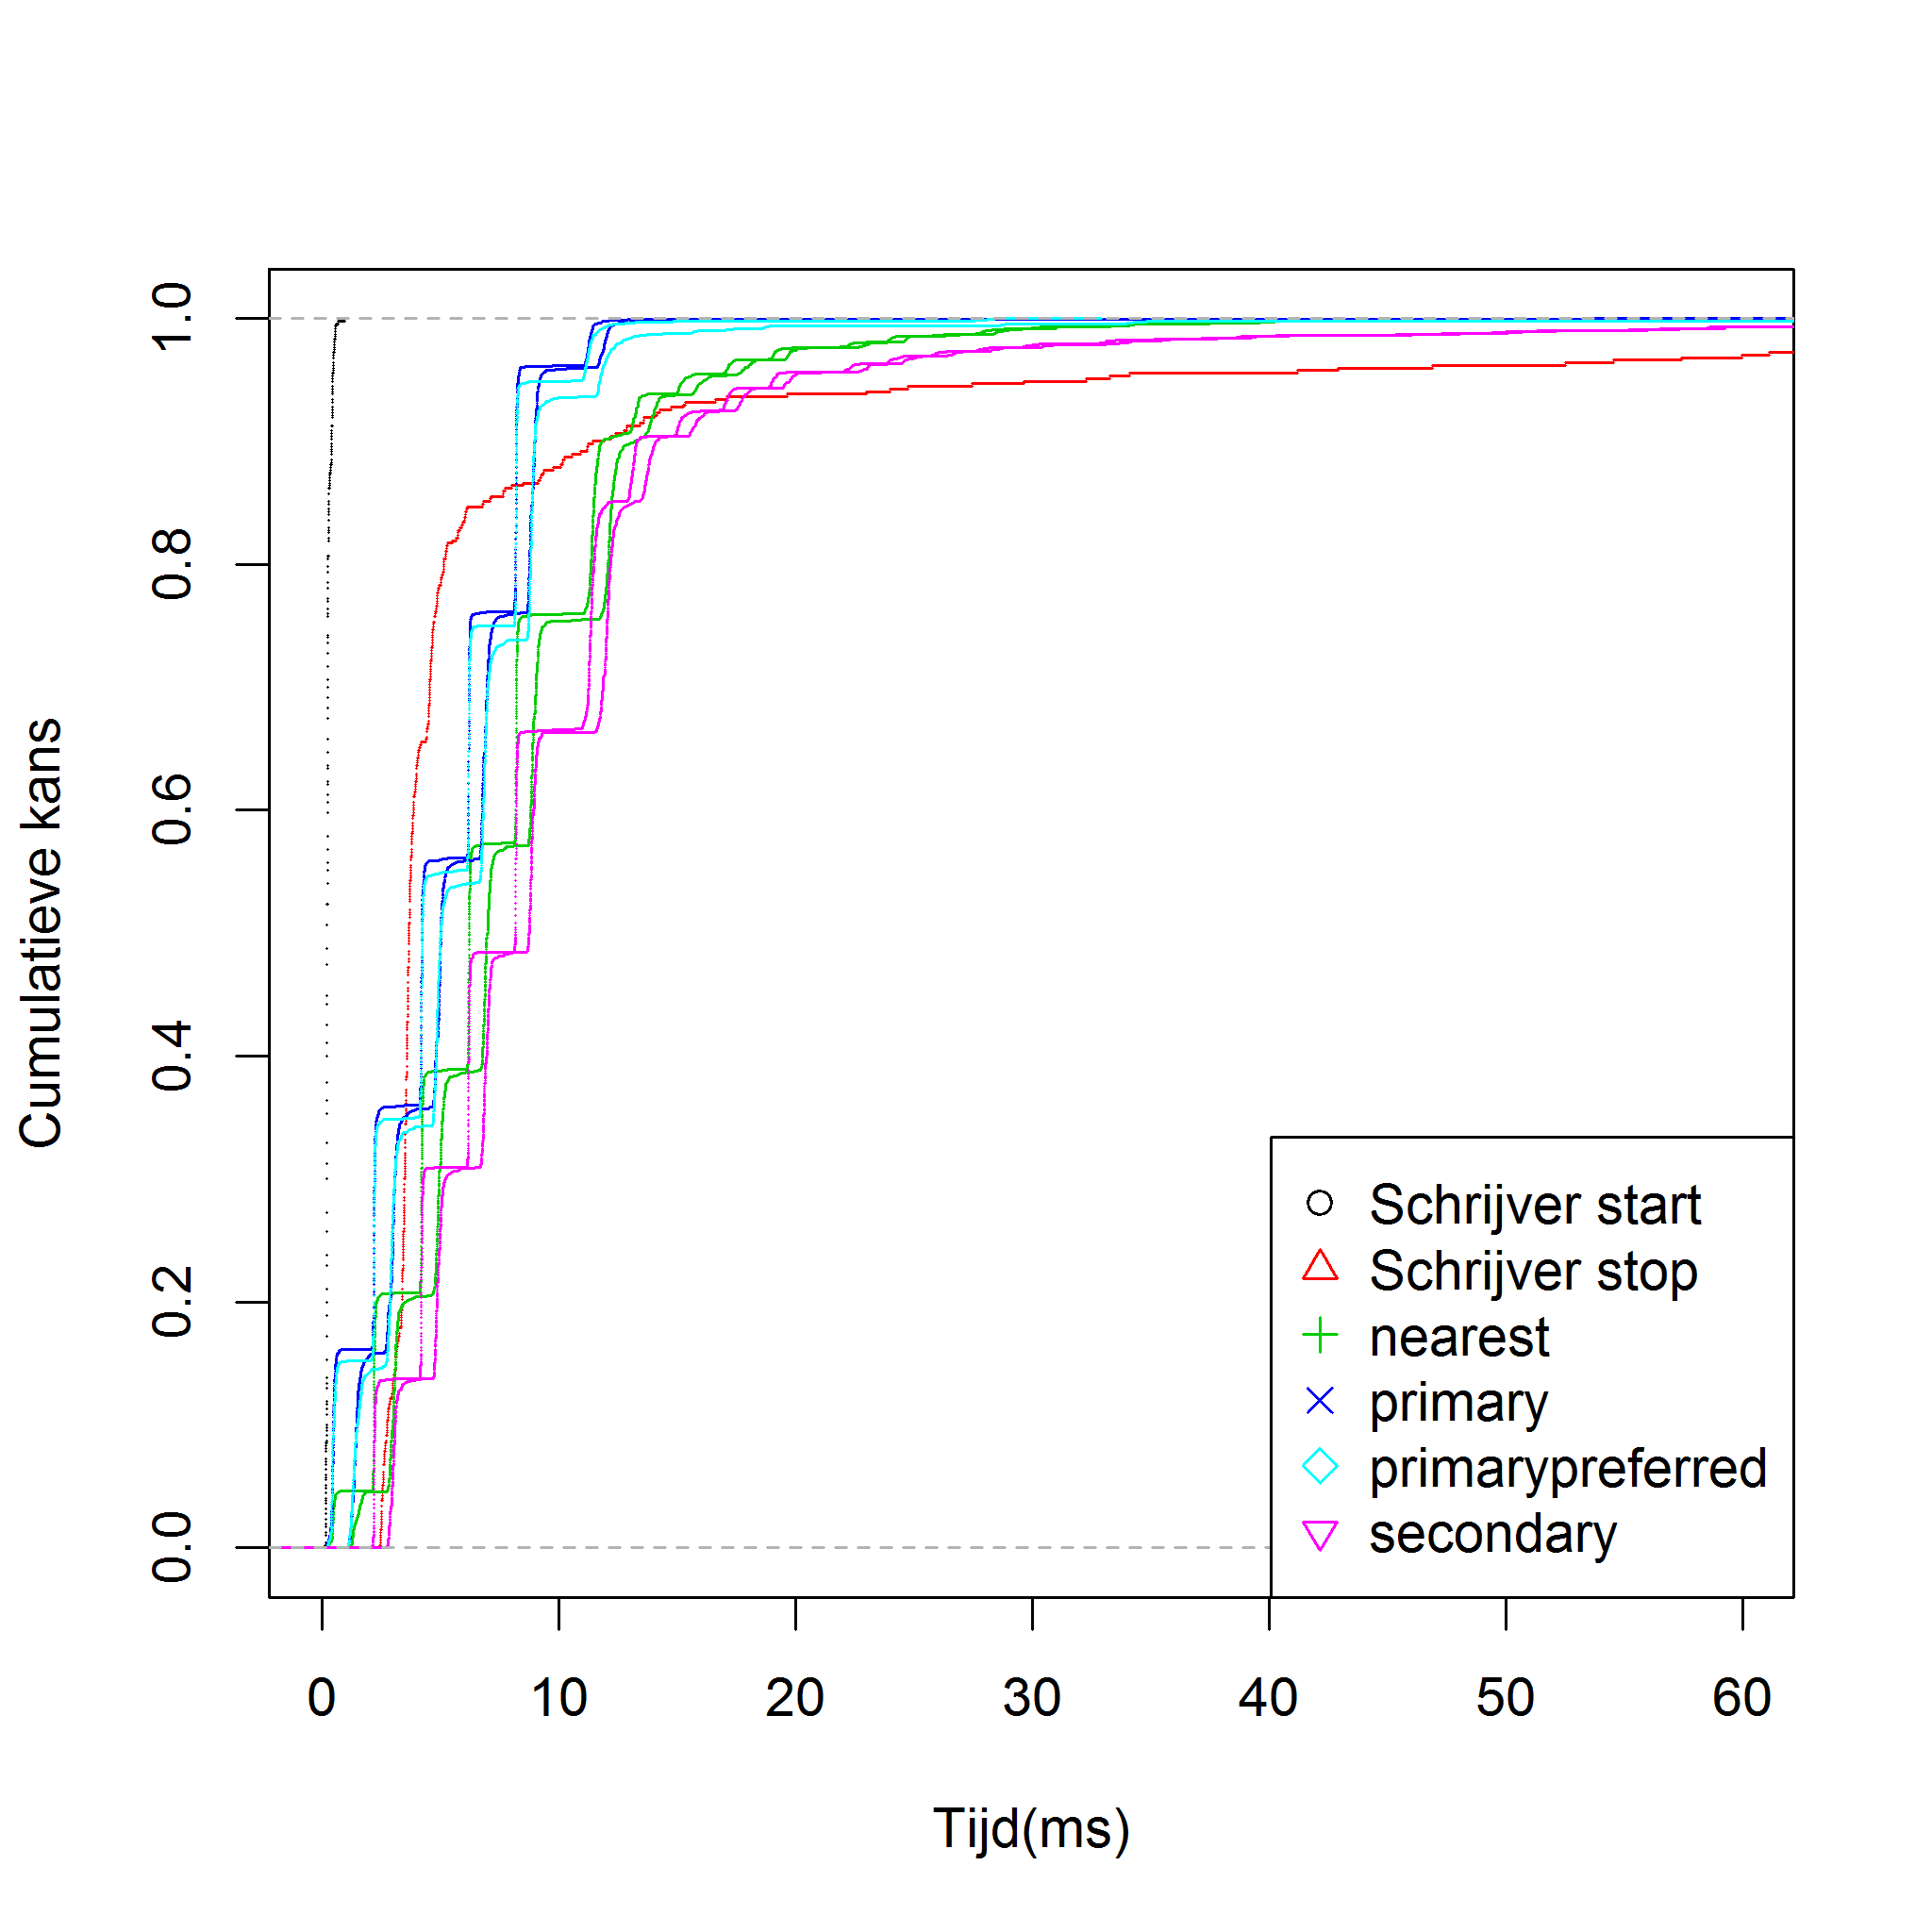
\includegraphics[width=.40\textwidth]{img/Observaties/MongoDB/ECDF-Reads-insert-majority-all-2}}
	\caption{Consistentie: Overzicht van MongoDB op de consistentie testen voor alle lezers gecombineerd met een 97-percentiel (voor de lezers) met start en stoptijden in dezelfde kleur. }
	\label{fig:consistentie-mongodb-all}
\end{figure}

\begin{figure}[ht!] 
	\centering
	\subfigure[Normal Update]{\label{fig:consistentie-mongodb-R2-normal} 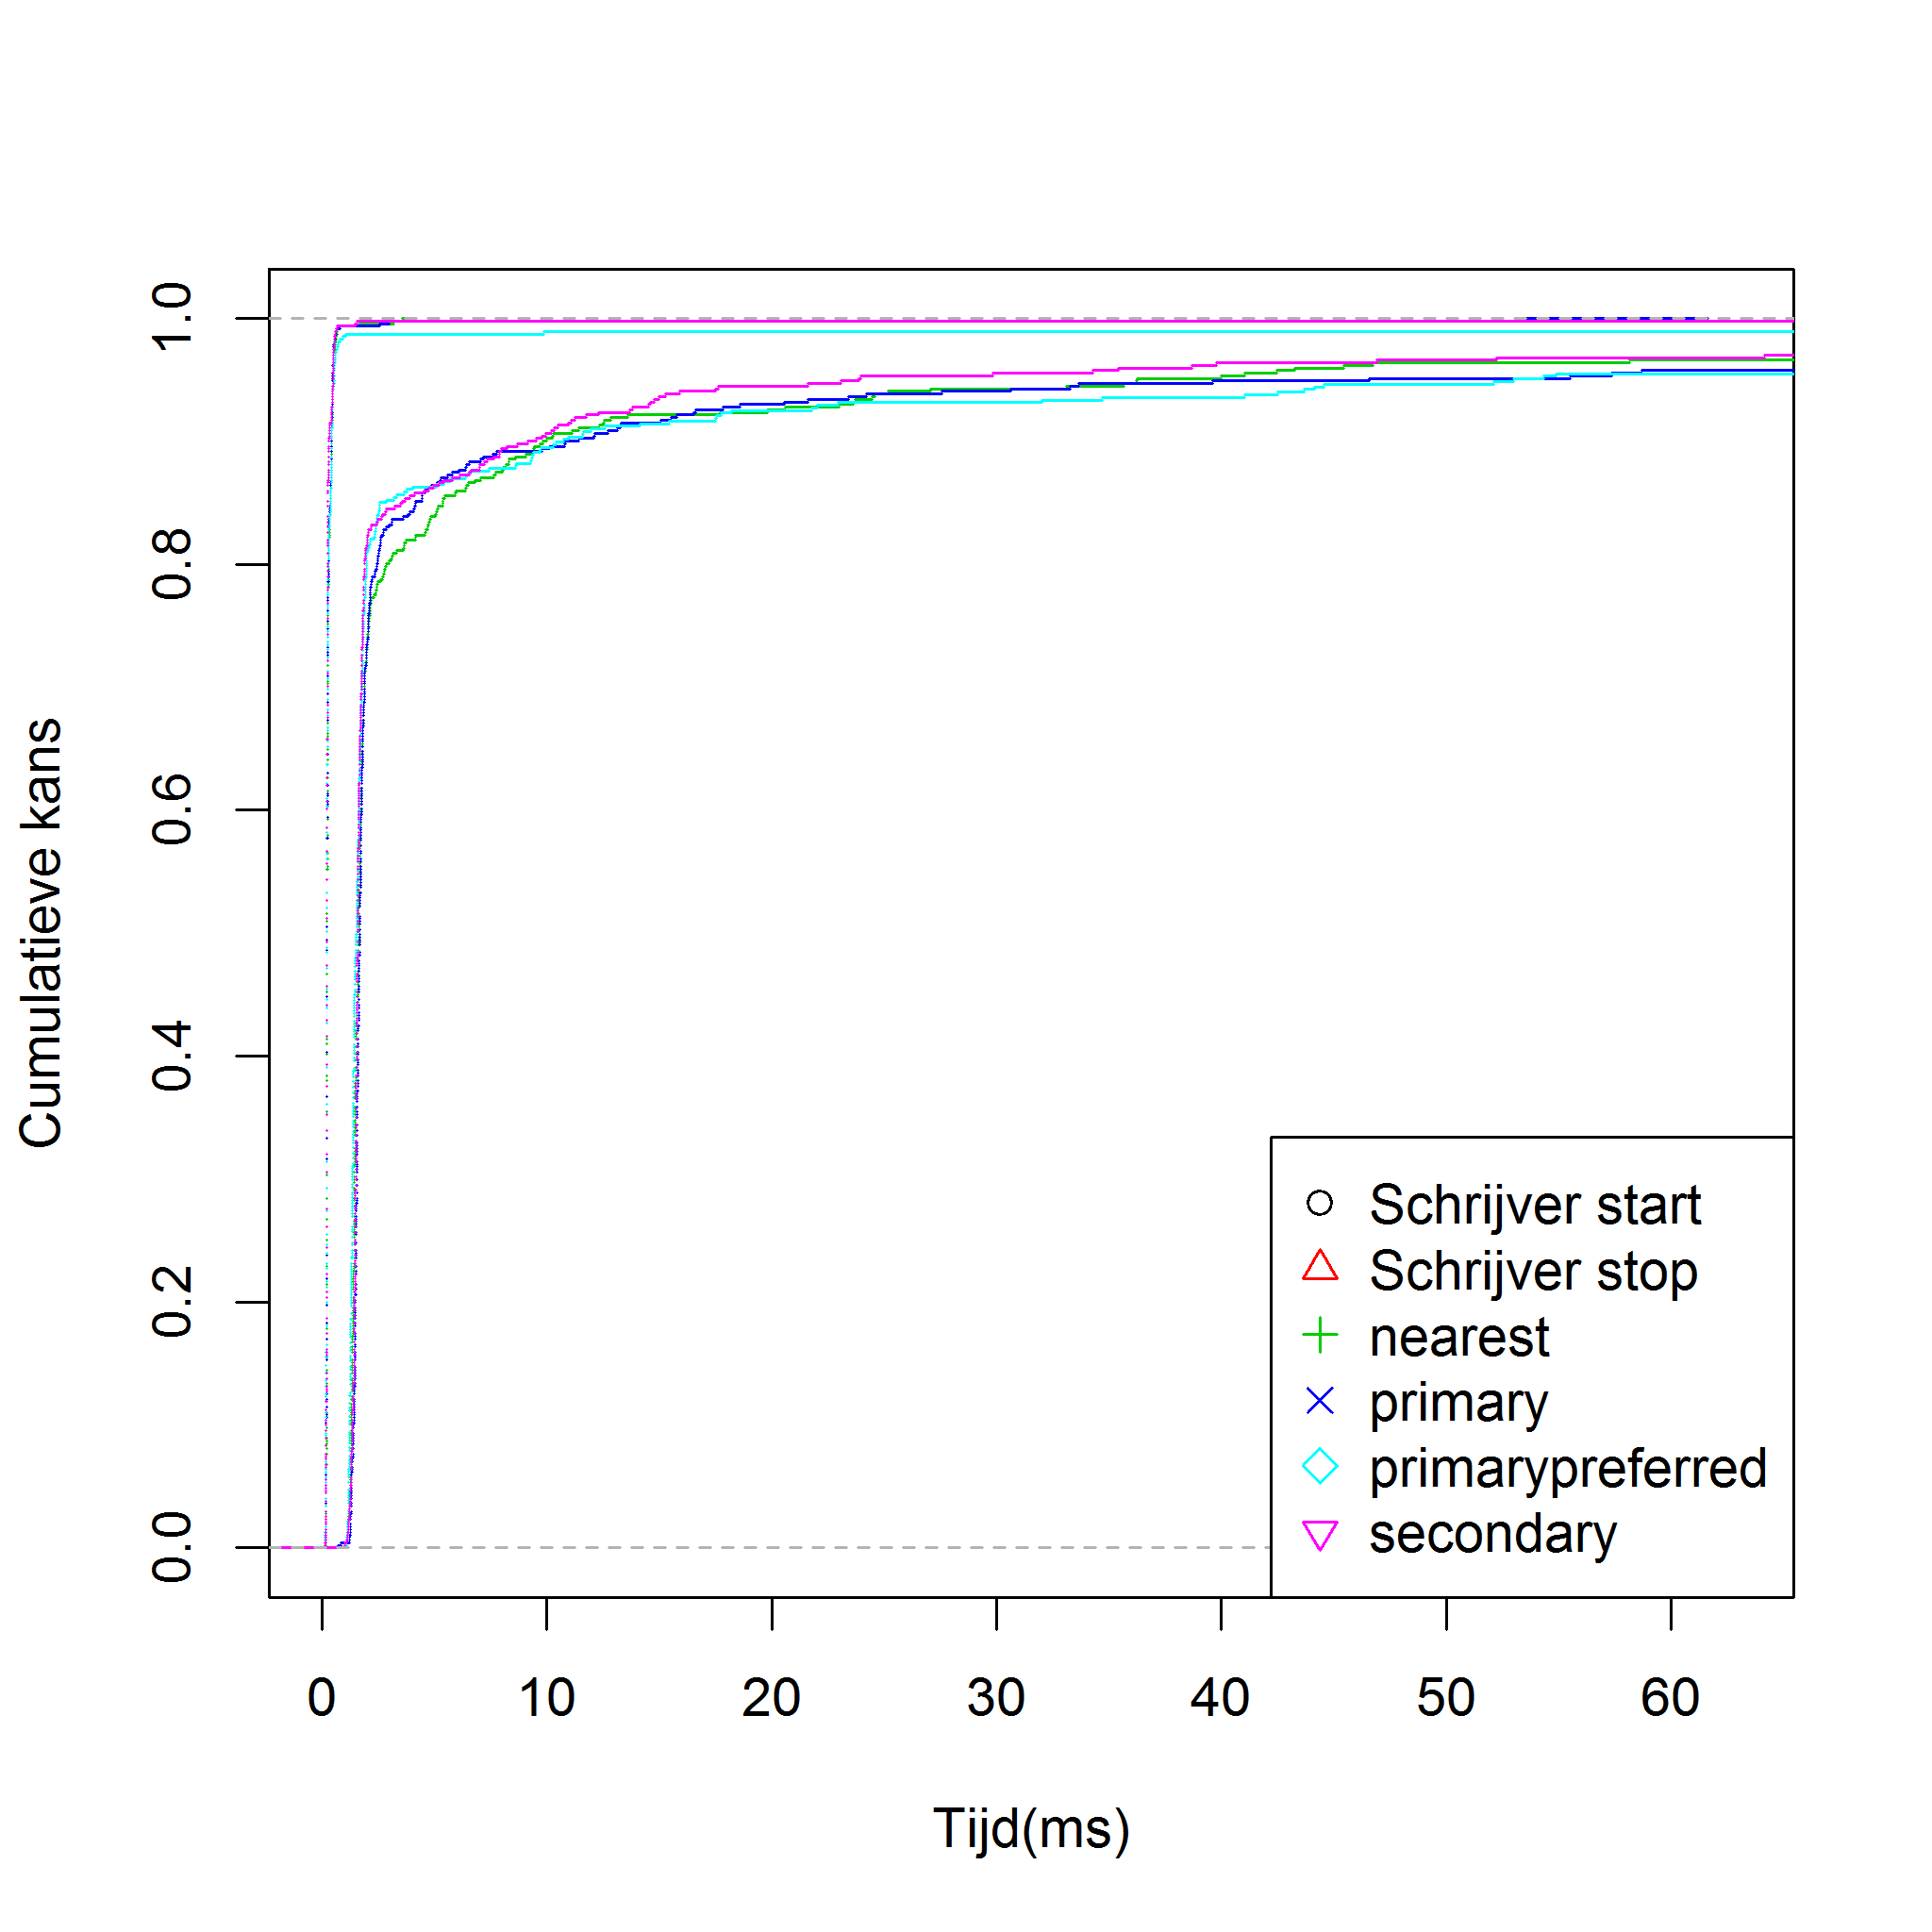
\includegraphics[width=.40\textwidth]{img/Observaties/MongoDB/ECDF-Reads-update-normal-1-2}}
	\subfigure[Safe Update]{\label{fig:consistentie-mongodb-R2-safe} 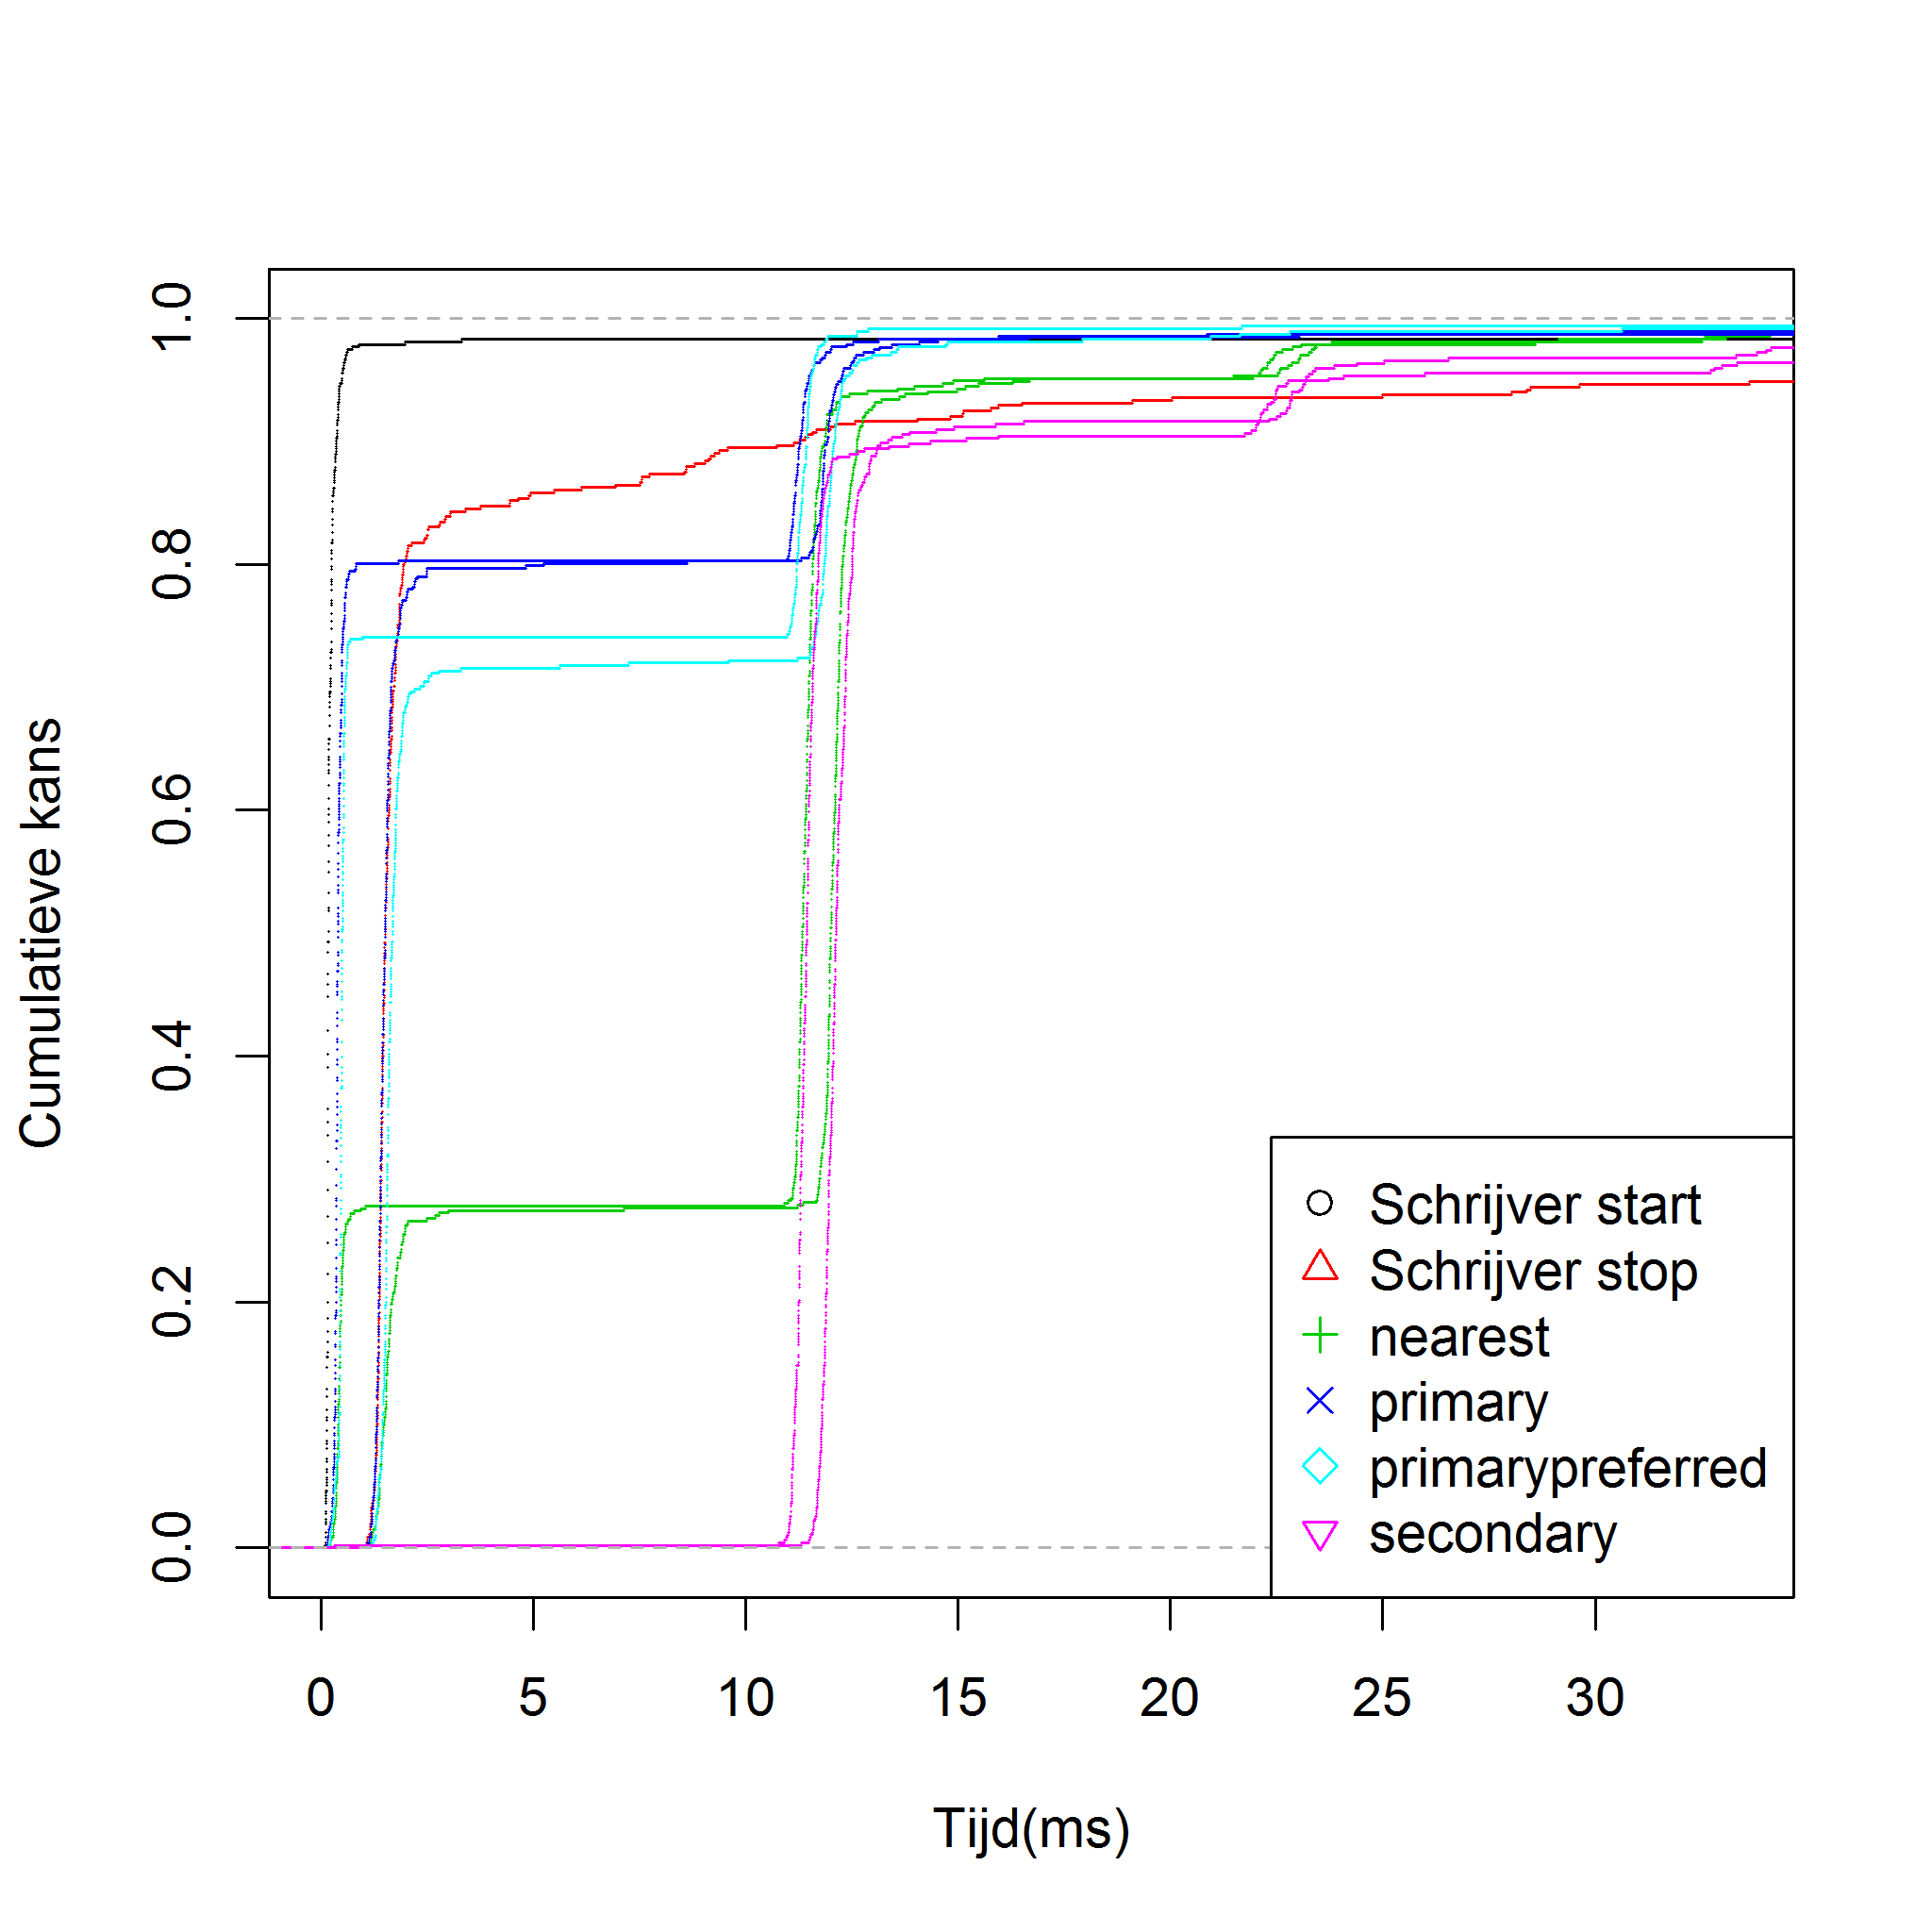
\includegraphics[width=.40\textwidth]{img/Observaties/MongoDB/ECDF-Reads-update-safe-1-2}}
	\subfigure[Fsync Safe Update]{\label{fig:consistentie-mongodb-R2-fsync} 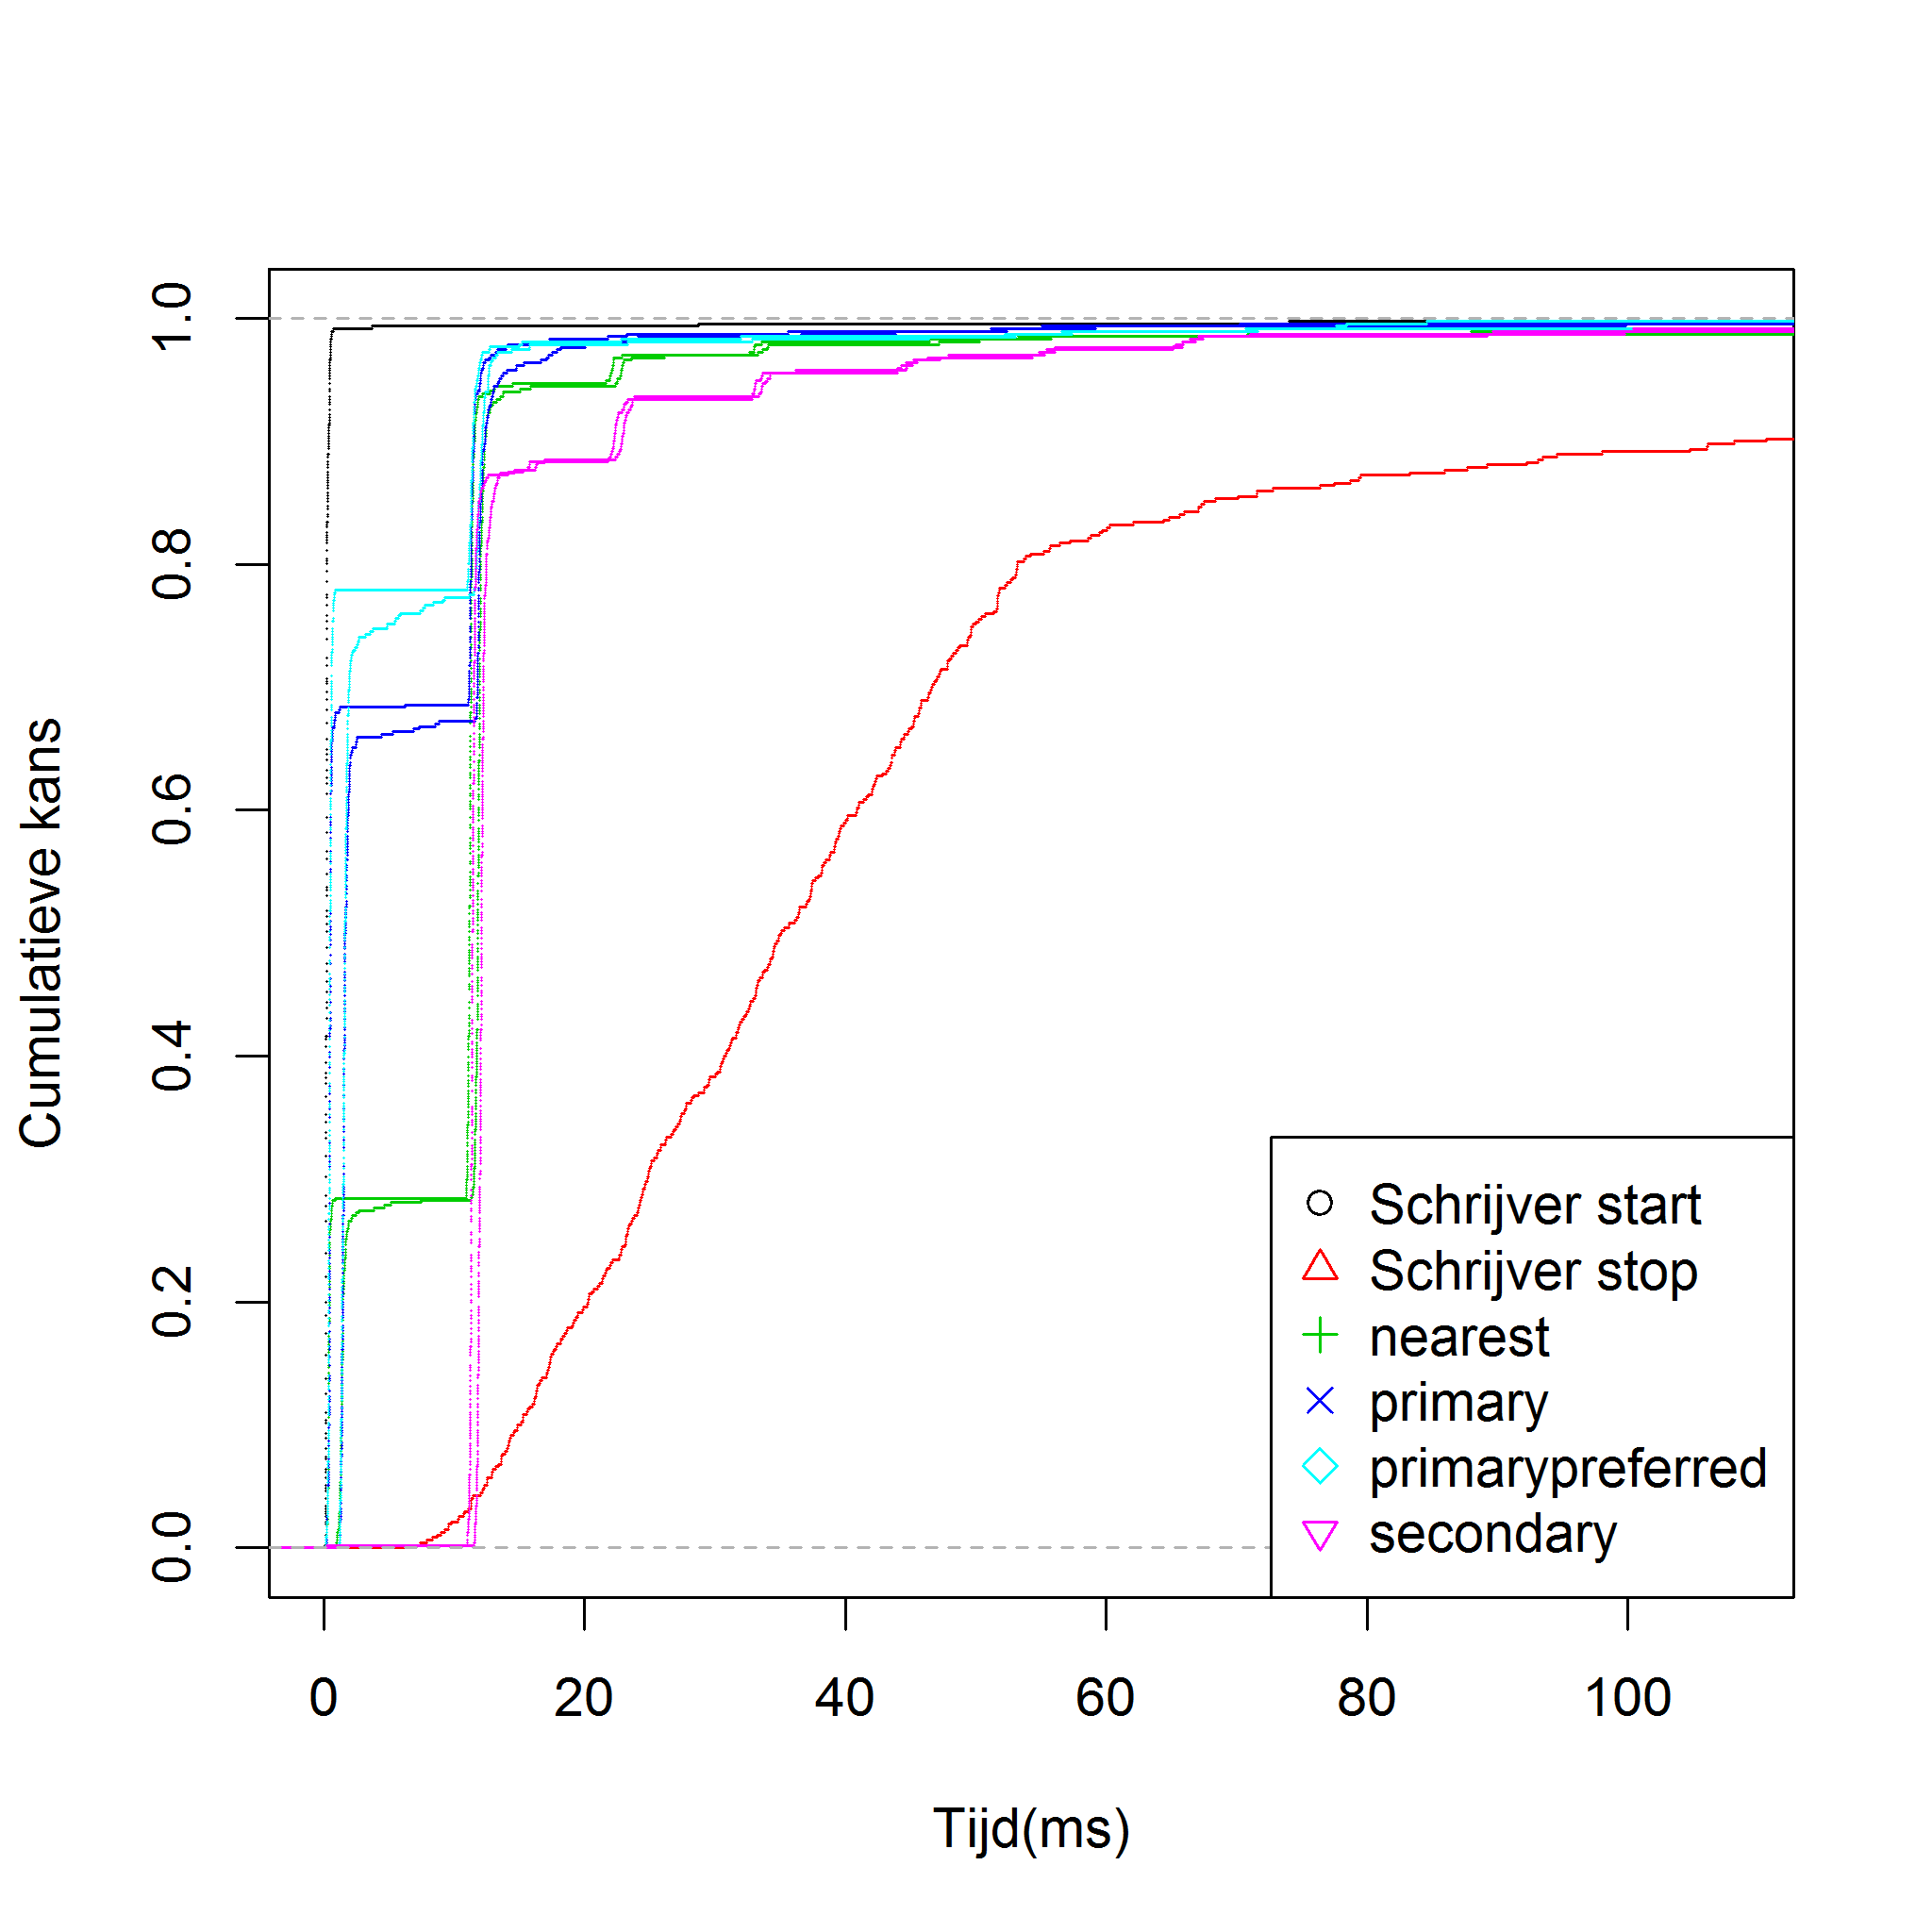
\includegraphics[width=.40\textwidth]{img/Observaties/MongoDB/ECDF-Reads-update-fsync_safe-1-2}}
	\subfigure[Replica Safe Update]{\label{fig:consistentie-mongodb-R2-replicasafe} 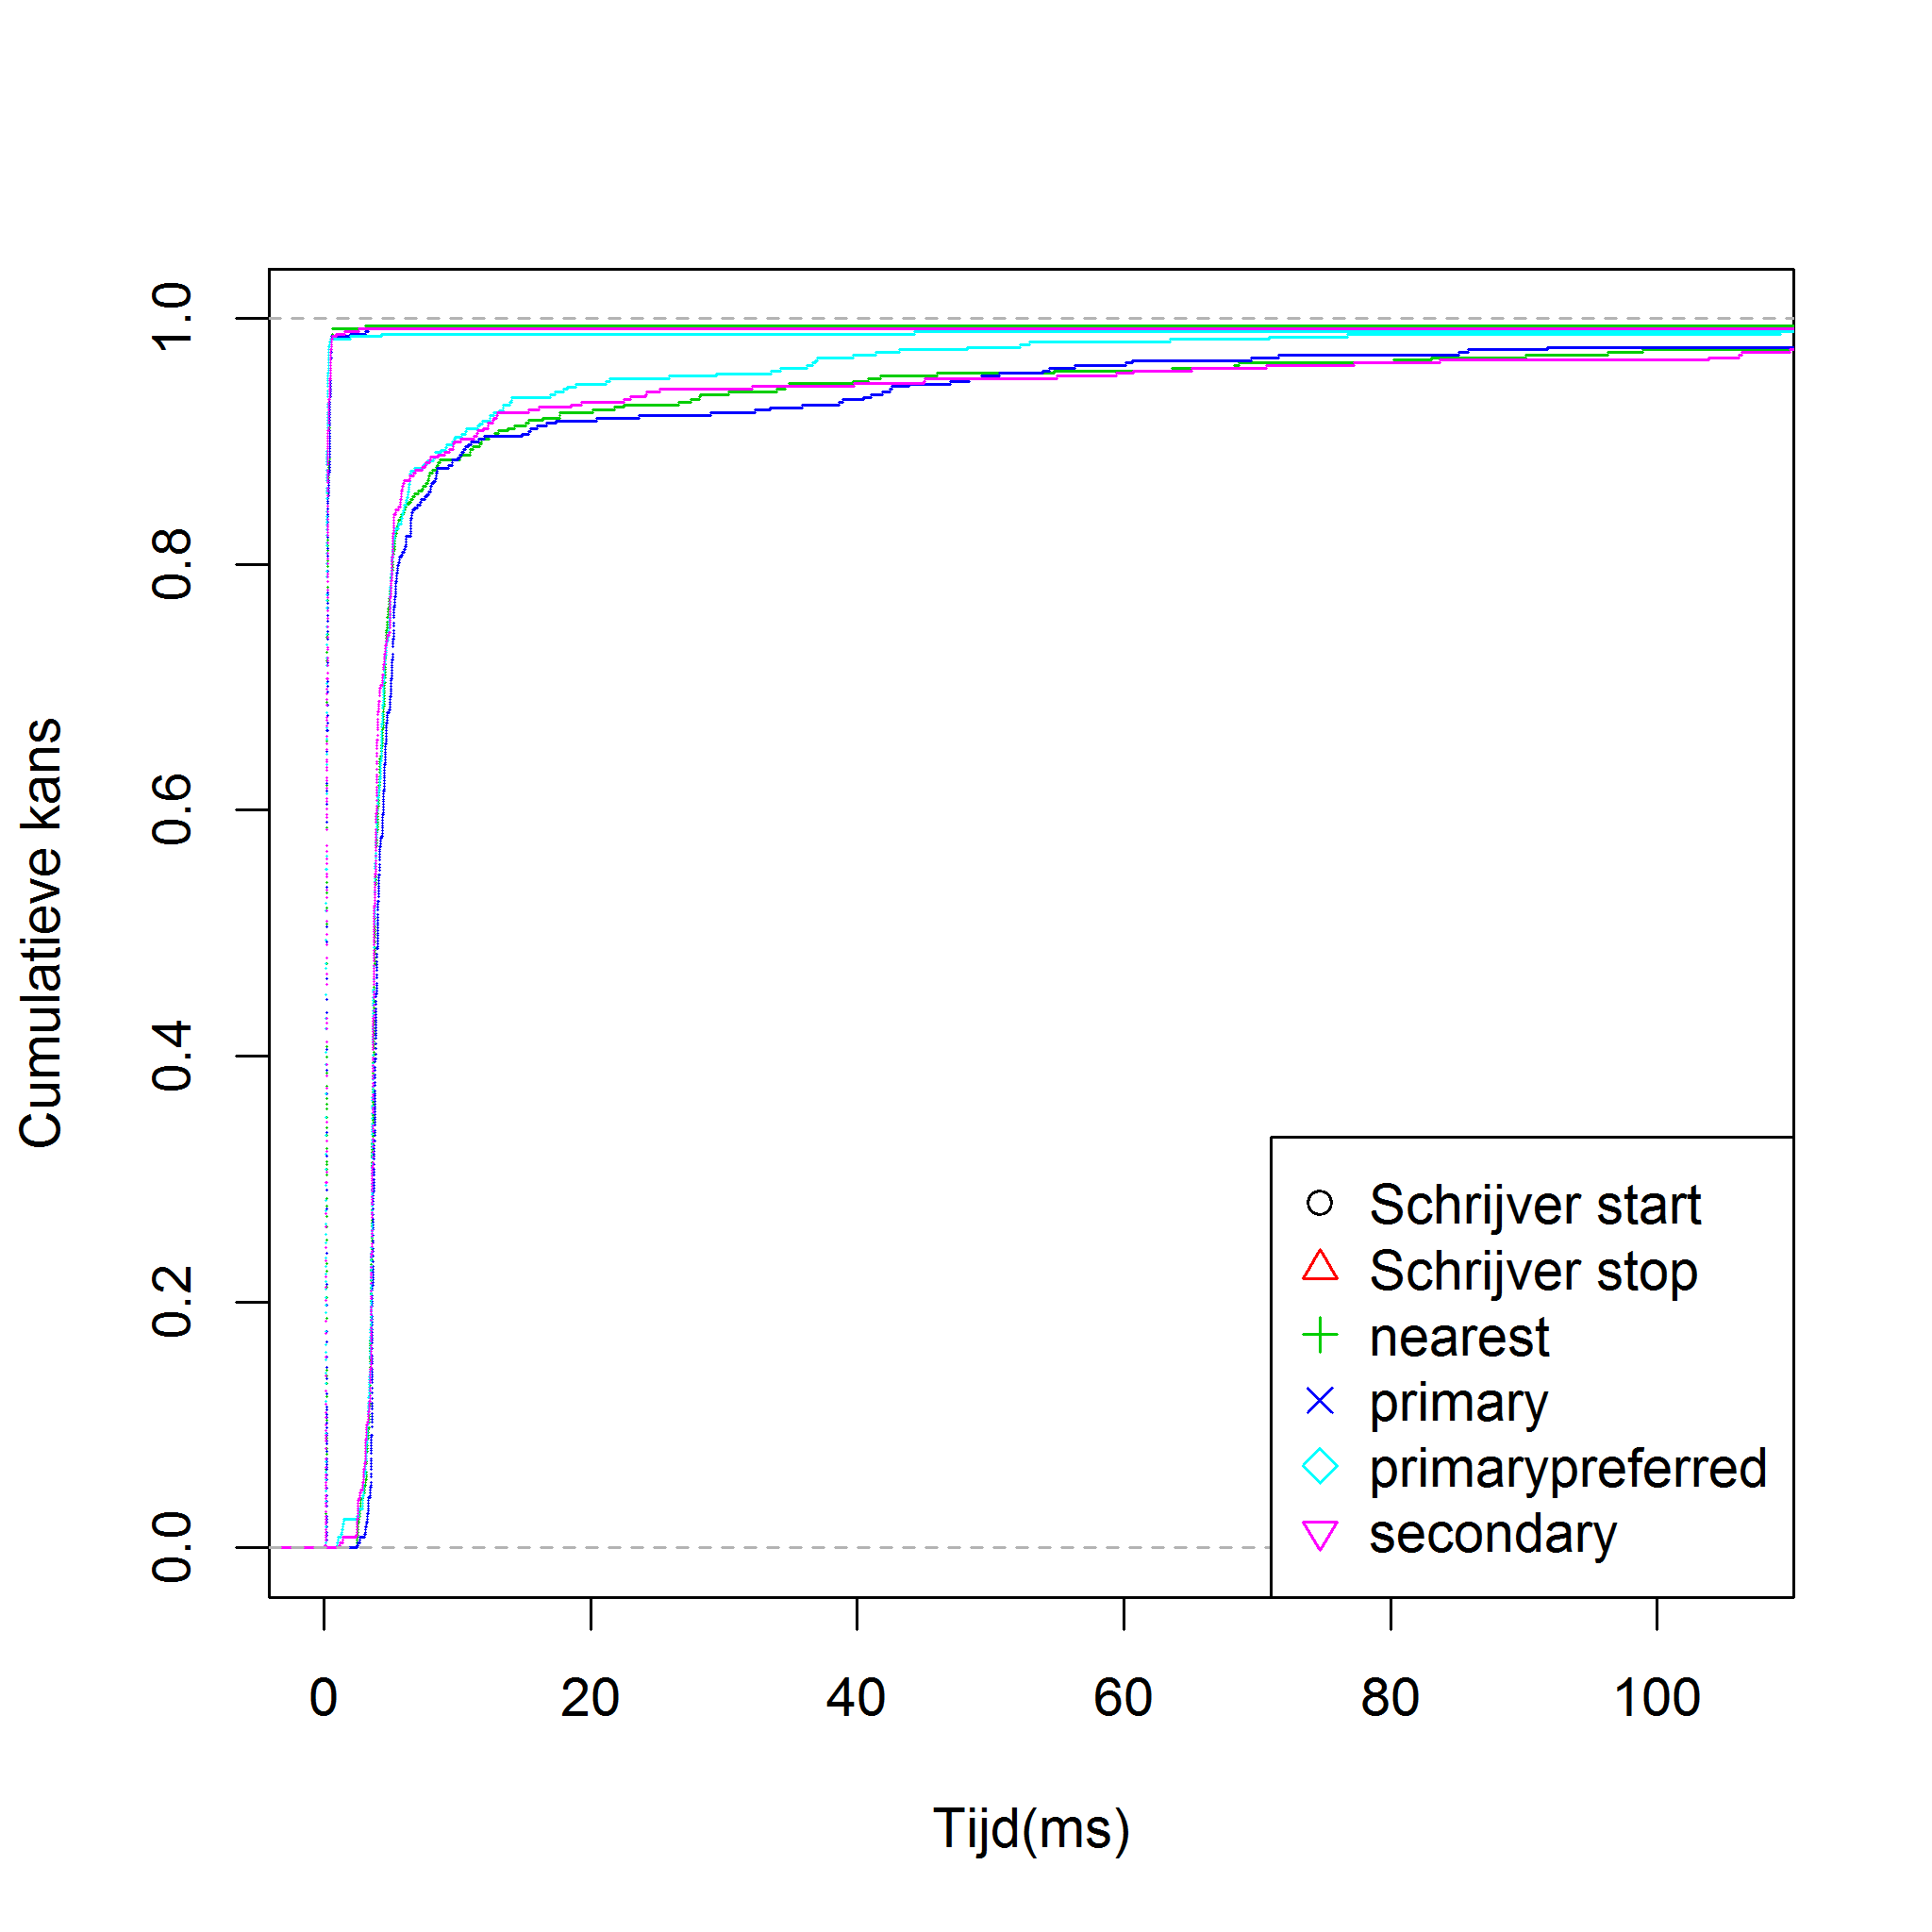
\includegraphics[width=.40\textwidth]{img/Observaties/MongoDB/ECDF-Reads-update-replicas_safe-1-2}}
	\subfigure[Majority Update]{\label{fig:consistentie-mongodb-R2-majority} 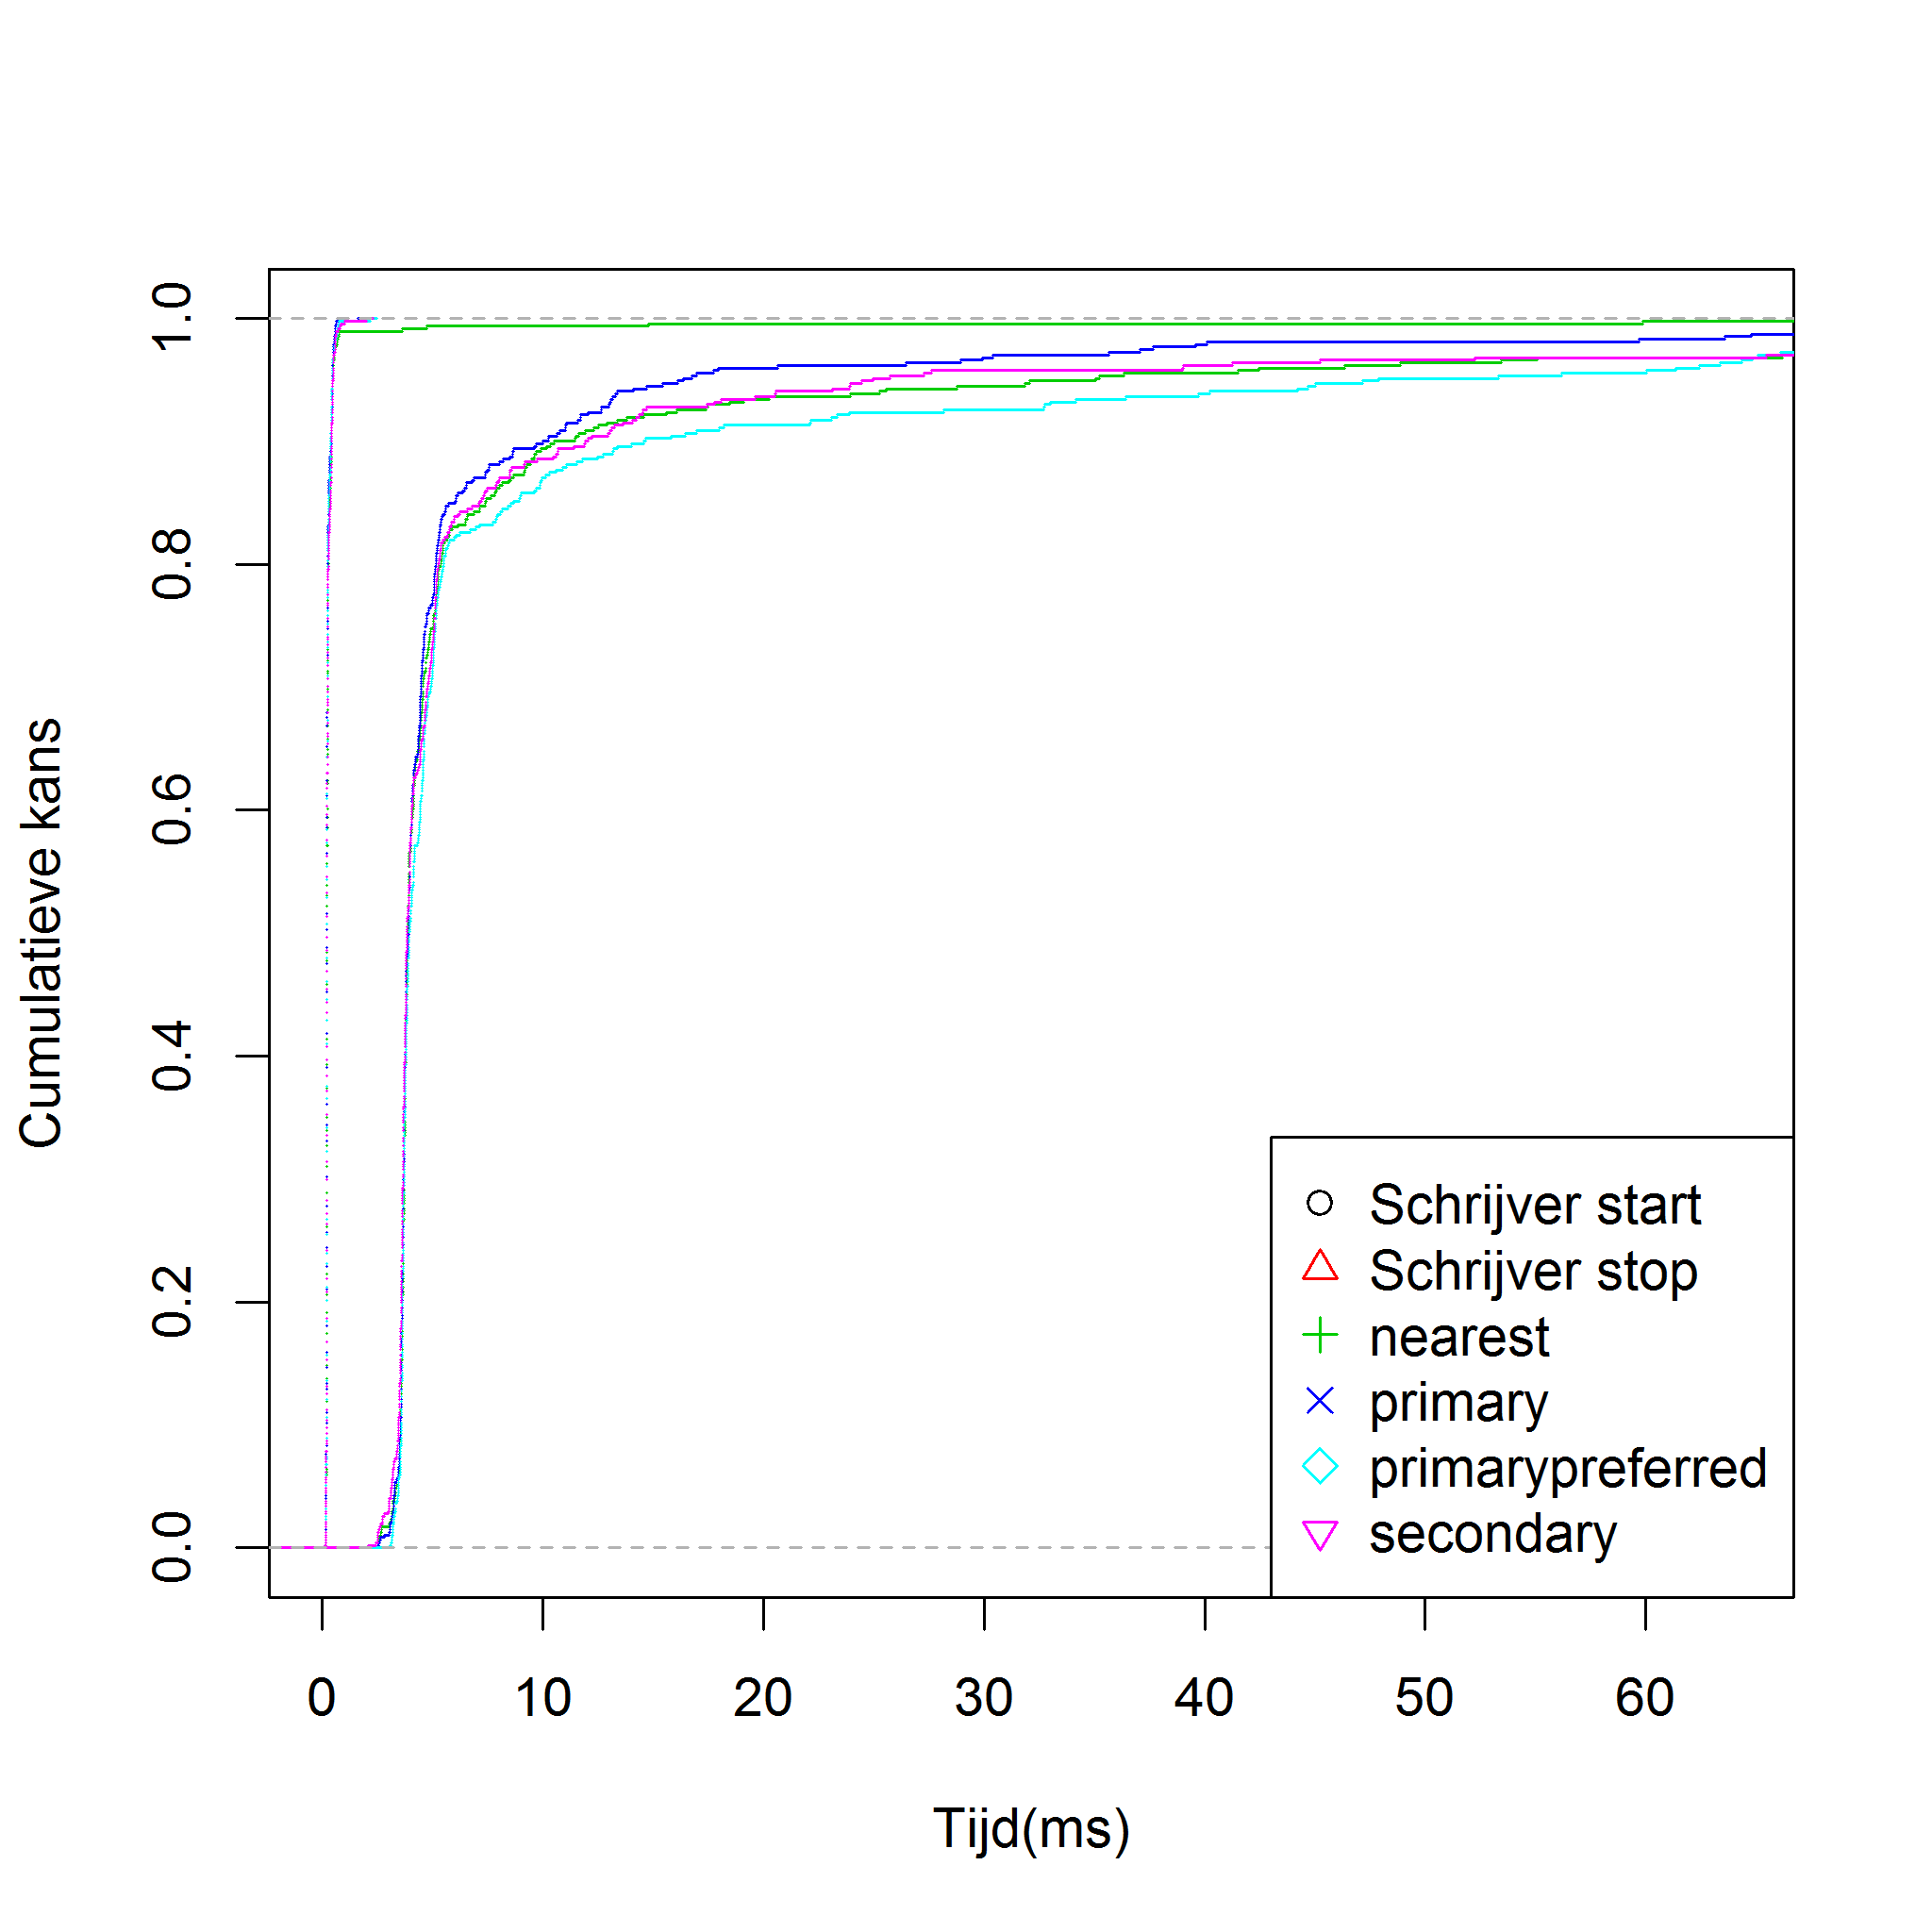
\includegraphics[width=.40\textwidth]{img/Observaties/MongoDB/ECDF-Reads-update-majority-1-2}}
	\subfigure[Majority Insert]{\label{fig:consistentie-mongodb-R2-majority-insert} 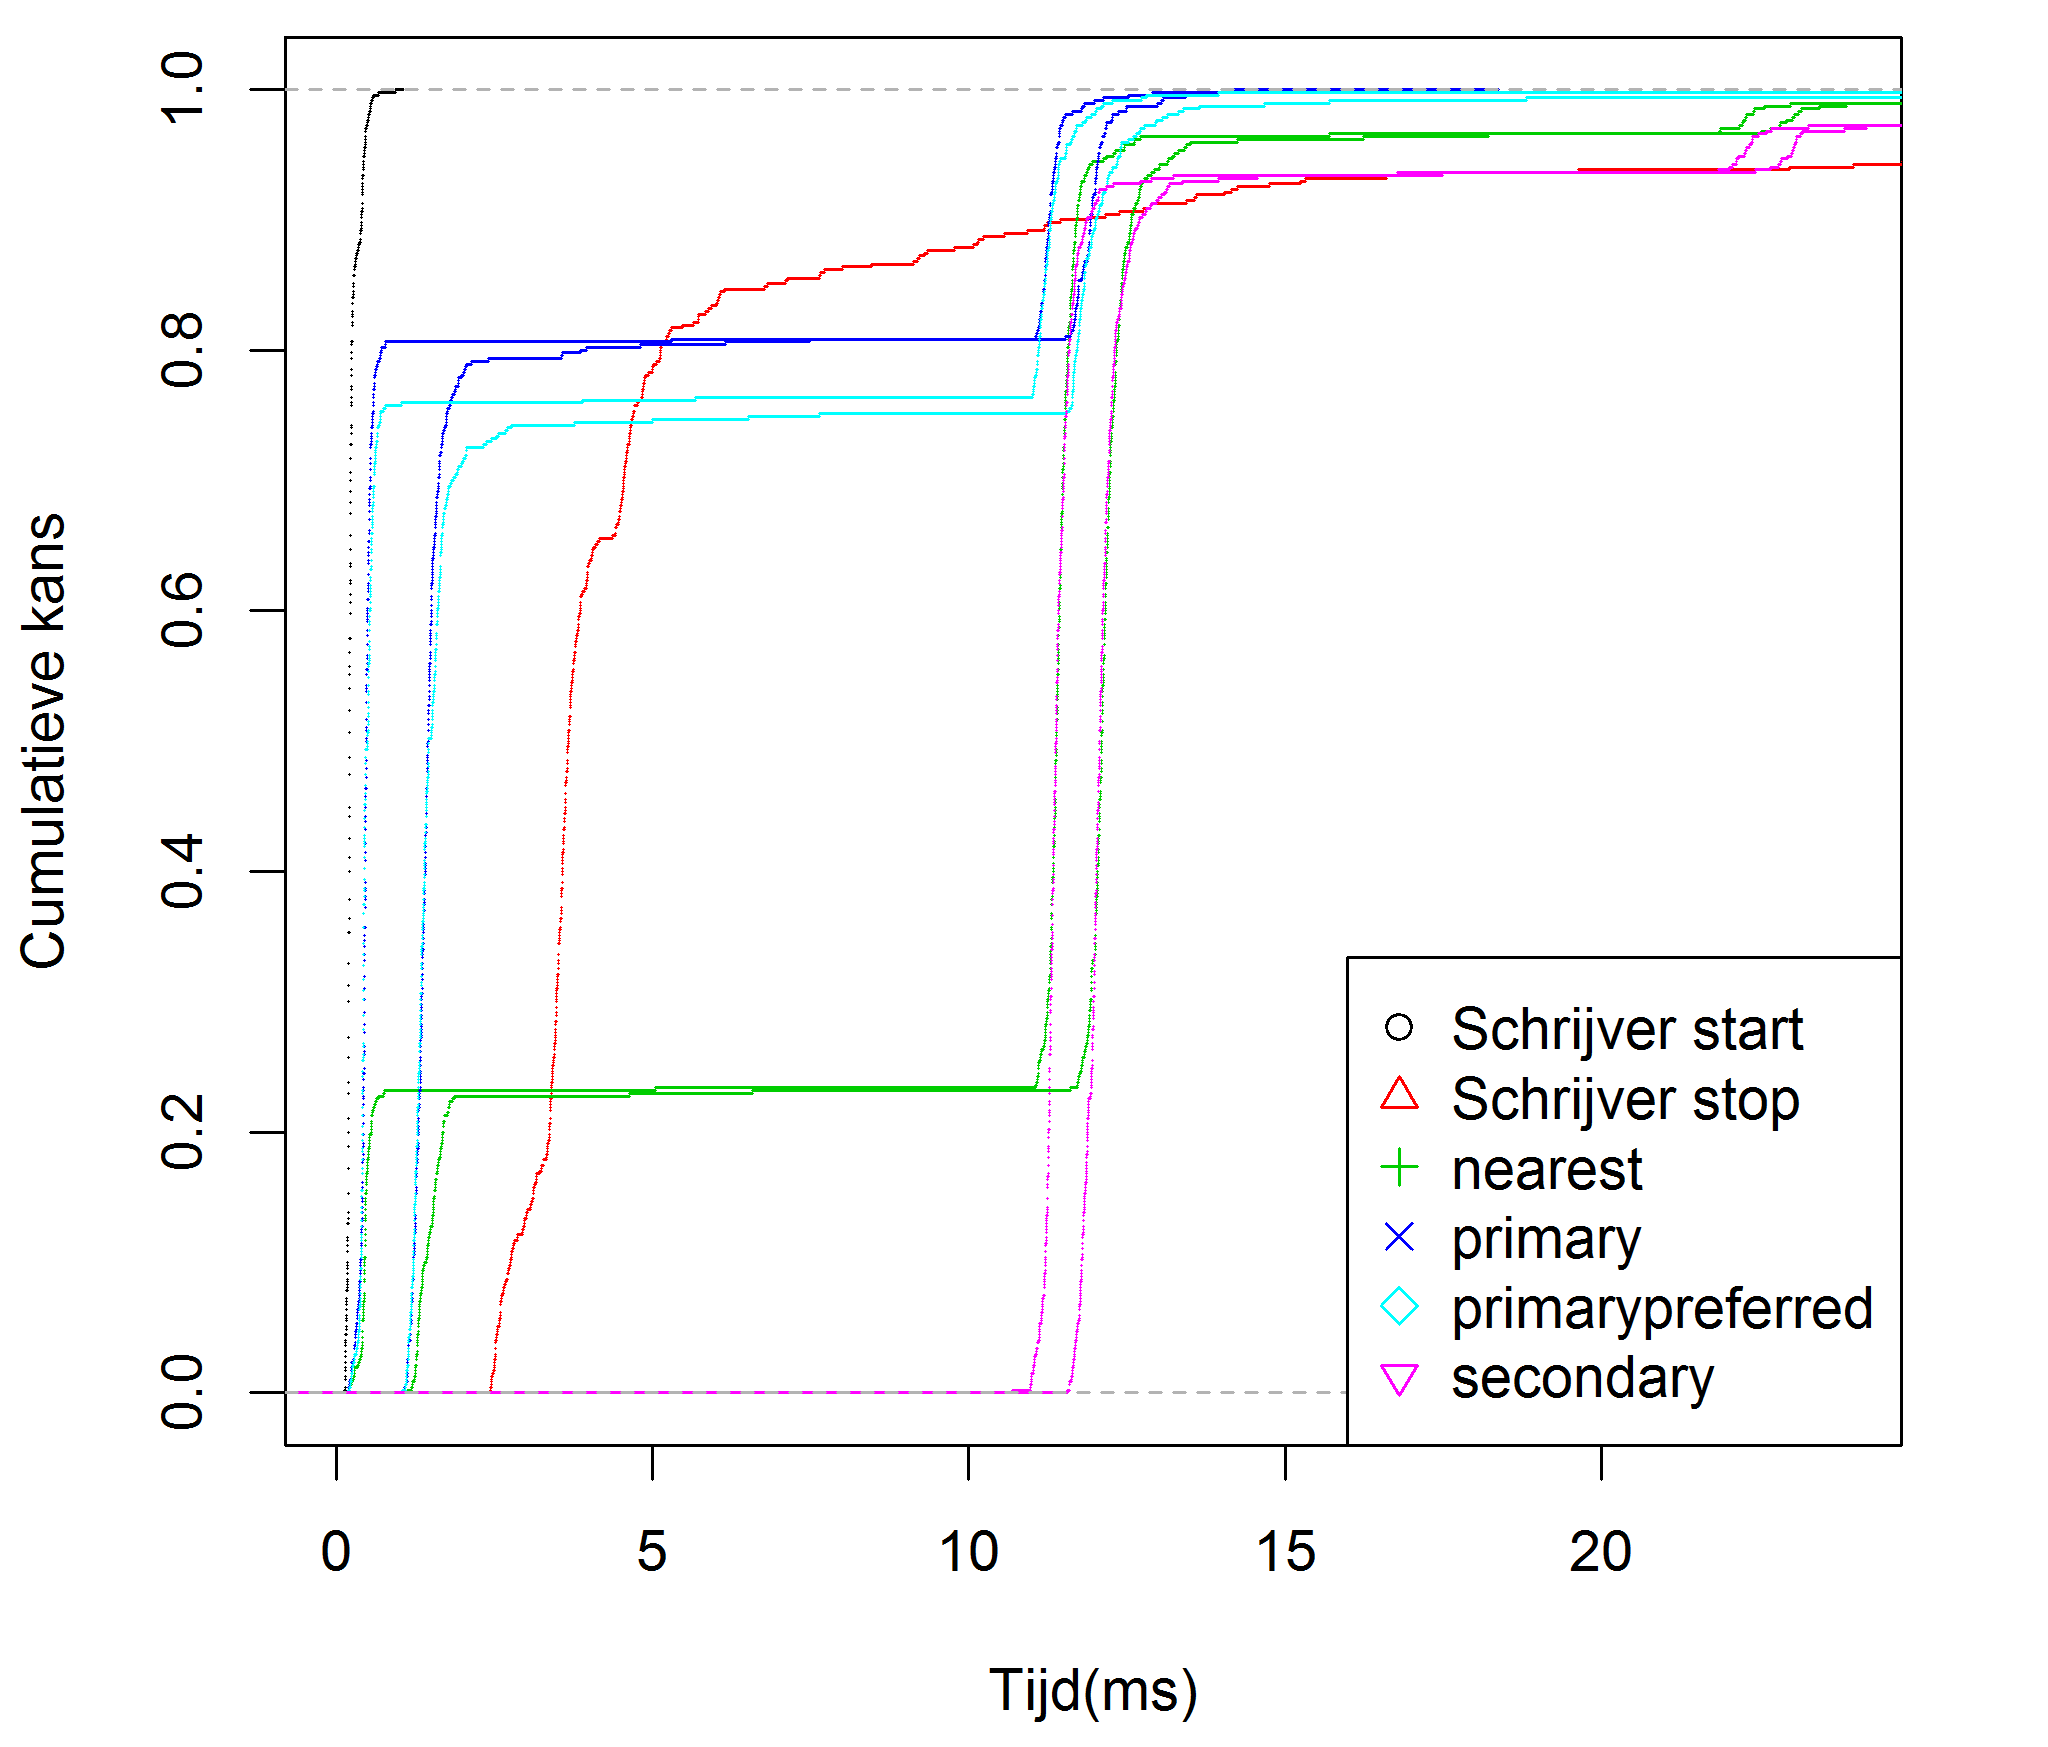
\includegraphics[width=.40\textwidth]{img/Observaties/MongoDB/ECDF-Reads-insert-majority-1-2}}
	\caption{Consistentie: Overzicht van MongoDB op de consistentie testen voor lezer 2 met een 99-percentiel (voor de lezers) met start en stoptijden in dezelfde kleur.}
	\label{fig:consistentie-mongodb-R2}
\end{figure}
